% Intended LaTeX compiler: pdflatex
\documentclass[letterpaper, 12pt]{report}
\usepackage[utf8]{inputenc}
\usepackage[T1]{fontenc}
\usepackage{graphicx}
\usepackage{longtable}
\usepackage{wrapfig}
\usepackage{rotating}
\usepackage[normalem]{ulem}
\usepackage{amsmath}
\usepackage{amssymb}
\usepackage{mathtools} % AW: added this to try to fix the ugly equation spacing around \sum
\usepackage{capt-of}
\usepackage{hyperref}
\usepackage{amsmath}		% Extra math definitions
\usepackage{bm}
\usepackage{breqn}
\usepackage{graphics}		% PostScript figures
\usepackage{setspace}		% 1.5 spacing
\usepackage{longtable}          % Tables spanning pages
\usepackage{natbib}
\usepackage{times}
\usepackage{url}
\usepackage{latexsym}
\usepackage[usenames]{color}
\usepackage{covington}
\usepackage{graphicx}
\usepackage{multirow}
\usepackage{subcaption}%#+LATEX_HEADER: \usepackage{subfigure}
\usepackage{booktabs}
\usepackage{tabularx}
\usepackage{adjustbox}
% \usepackage{subfigure}
% \usepackage[T1]{fontenc}
% \usepackage[utf8]{inputenc}
\usepackage{enumitem}
\usepackage[english]{babel}
\usepackage{blindtext}
\usepackage{amsfonts}
\usepackage{amsthm}
\usepackage[table,xcdraw]{xcolor}
\usepackage{rotating}
\usepackage{listings}
\definecolor{NiceBlue}{RGB}{11, 102, 163}
\definecolor{SlightRed}{RGB}{249,38,114}
\usepackage{textcomp} % other glyphs needed for upquote in listings below
\lstdefinelanguage{DemoExample}
{ basicstyle=\footnotesize \ttfamily,
commentstyle=\color{SlightRed} \rmfamily\itshape,
stringstyle=\color{NiceBlue},
morecomment=[s]{/*}{*/},
morestring=[b]'
}
\usepackage[fancyhdr]{macros/McECEThesis}	% Thesis style
\usepackage{McGillLogo}		% McGill University crest
\usepackage{color}
\insidemargin = 1.1in
\outsidemargin = 1.1in
\abovemargin = 1.1in
\belowmargin = 0.75in
\newcommand{\beq}{\begin{equation}}
\newcommand{\eeq}{\end{equation}}
\usepackage{palatino}           % Less abusive fonts
\usepackage{macros/palatcm}
\usepackage{hyperref}
\let\mathexp=\exp %redefine \exp to \mathexp cuz gb4e package redefines \exp
\usepackage{gb4e}
\noautomath
\usepackage[acronym,toc,section=section]{glossaries}

\makeglossaries

% GLossary entries
\newglossaryentry{tlm}{name=Transformers,description={{A class of models first derived by Vaswani et al. 2017}}}
% Acronyms
\newacronym{llm}{LLMs}{Large Language Models}
\newacronym{nlu}{NLU}{Natural Language Understanding}
\newacronym{bb}{BB}{branch and bound}


\newcommand{\xhdr}[1]{{\noindent\bfseries #1}.}
\def\Snospace~{\S{}} % If i don't add this overleaf complains
\renewcommand{\sectionautorefname}{\Snospace}
\renewcommand{\subsectionautorefname}{\Snospace}
\newcommand\boldred[1]{\textcolor{red}{\textbf{#1}}}
\newcommand\boldblue[1]{\textcolor{blue}{\textbf{#1}}}


\DeclareMathOperator*{\argminB}{argmin}

\newcommand{\PermAcc}{Permutation Acceptance} % a macro

\author{Koustuv Sinha}
\date{}
\title{PhD Thesis}
\hypersetup{
 pdfauthor={Koustuv Sinha},
 pdftitle={PhD Thesis},
 pdfkeywords={},
 pdfsubject={},
 pdfcreator={Emacs 28.1 (Org mode 9.6)}, 
 pdflang={English}}
\begin{document}

\maketitle
\raggedbottom
\spacing{1.5}%\onehalfspacing
\pagenumbering{roman}

\chapter*{Acknowledgements}
\label{sec:org111920c}
\chapter*{Abstract}
\label{sec:orgec62e8c}
\chapter*{Abstract in French}
\label{sec:org71795cd}
\chapter*{Contributions to Original Knowledge}
\label{sec:org3bc5b8a}
\chapter*{Contributions of Authors}
\label{sec:org2435b5a}

\listoffigures{}

\listoftables{}

\clearpage
\setcounter{tocdepth}{3}
\tableofcontents

\clearpage

\pagenumbering{arabic}

\chapter{Introduction}
\label{sec:orgeb32902}

\textbf{\textbf{Central Theme of the thesis}} : Understanding systematicity in pre-trained language models through semantic and syntactic generalization.

In this thesis I discuss my work on understanding systematicity in pre-trained language models.

\clearpage

\chapter{Background}
\label{sec:orgaa03e11}

\section{Early methods for text representation}
\label{sec:org7176877}
\section{Neural Inductive bias of text representation}
\label{sec:org2479903}
\subsection{Feed Forward Neural Networks}
\label{sec:orgc5c64b1}
\subsection{Recurrent Neural Networks}
\label{sec:org081fc19}
\subsection{Transformer Models}
\label{sec:orgce0ee81}

\gls{llm} are the state-of-the-art in language models, which are based on \gls{tlm}.
\section{Pre-training and the advent of Large Language Models}
\label{sec:org754bcf3}
Success of pre-training and scale
\section{Systematicity and Generalization}
\label{sec:orgb799e4e}
\subsection{Definitions}
\label{sec:org70d8bf6}
\begin{enumerate}
\item Systematicity
\label{sec:orgbb21691}
\item Word Order Sensitivity
\label{sec:org41a33eb}
\end{enumerate}
\subsection{Tasks}
\label{sec:org51f5f2f}


\clearpage

\chapter{Understanding semantic generalization through systematicity}
\label{chap:clutrr}

\gls{nlu} systems have been extremely successful at reading comprehension tasks, such as question answering (QA) and natural language inference (NLI).
These tasks typically test for semantic generalization, where a model has to understand the meaning of the input sentence / passage in order to perform the given task.
An array of existing datasets are available for these tasks. This includes datasets that test a system's ability to extract factual answers from text \citep{Rajpurkar2016-yc,Nguyen2016-ec,Trischler2016-fc,Mostafazadeh2016-hu,Su2016-so}, as well as datasets that emphasize commonsense inference, such as entailment between sentences \citep{bowman2015large,williams2018broad}.

However, there are growing concerns regarding the ability of \acrshort{nlu} systems---and neural networks more generally---to generalize in a systematic and robust way \citep{bahdanau2018systematic,lake2017generalization,Johnson2016-mw}.
For instance, recent work has highlighted the brittleness of \acrshort{nlu} systems to adversarial examples \citep{jia2017adversarial}, as well as the fact that \acrshort{nlu} models tend to exploit statistical artifacts in datasets, rather than exhibiting true reasoning and generalization capabilities \citep{gururangan2018annotation,kaushik2018much}.
These findings have also dovetailed with the recent dominance of large pre-trained language models, such as BERT, on \acrshort{nlu} benchmarks \citep{devlin2018bert,peters2018deep}, which suggest that the primary difficulty in these datasets is incorporating the statistics of the natural language, rather than reasoning.

An important challenge is thus to develop \acrshort{nlu} benchmarks that can precisely test a model's capability for robust and systematic generalization.
Ideally, we want language understanding systems that can not only answer questions and draw inferences from text, but that can also do so in a systematic, logical, and robust way.
While such reasoning capabilities are certainly required for many existing \acrshort{nlu} tasks, most datasets combine several challenges of language understanding into one, such as co-reference/entity resolution, incorporating world knowledge, and semantic parsing---making it difficult to isolate and diagnose a model's capabilities for systematic generalization and robustness.

In this work, we propose to use the properties of \textit{systematicity} to test the limits of semantic generalization of modern neural networks. As defined by \citet{fodor1988connectionism}, systematicity test the ability of a system to understand the recombination of known parts and rules. Thus, inspired by the classic AI challenge of inductive logic programming \citep{Quinlan1990-iv}, in this chapter I discuss my work on developing semi-synthetic benchmark designed to explicitly test an \acrshort{nlu} model's ability for systematic and robust logical generalization \citep{sinha-etal-2019-clutrr}.
Our benchmark suite---termed \textbf{CLUTRR} (Compositional Language Understanding and Text-based Relational Reasoning)---contains a large set of semi-synthetic stories involving hypothetical families.
Given a story, the goal is to infer the relationship between two family members, whose relationship is not explicitly mentioned.
To solve this task, a learning agent must extract the relationships mentioned in the text, induce the logical rules governing the kinship relationships (e.g., the transitivity of the sibling relation), and use a combination of these rules to infer the relationship between a given pair of entities.
Crucially, the CLUTRR benchmark allows us to test a learning agent's ability for \emph{systematic generalization} by testing on stories that contain unseen combinations of logical rules.
CLUTRR also allows us to precisely test for the various forms of \emph{model robustness} by adding different kinds of superfluous \emph{noise facts} to the stories.


\section{Technical Background}
\label{sec:clutrr_bg}

\subsection{Notations and Terminology}

Following standard practice in formal semantics, we use the term \textit{atom} to refer to a \textit{predicate} symbol and a list of terms, such as $[\texttt{grandfatherOf},X,Y]$, where the predicate $\texttt{grandfatherOf}$ denotes the \textit{relation} between the two \textit{variables}, $X$ and $Y$. We restrict the predicates to have an arity of 2, i.e.,  binary predicates.
A logical \textit{rule} in this setting is of the form $\mathcal{H} \vdash \mathcal{B}$, where $\mathcal{B}$ is the \textit{body} of the rule, i.e., a conjunction of two \textit{atoms} ($[\alpha_1,\alpha_2]$) and $\mathcal{H}$ is the \textit{head}, i.e., a single \text{atom} ($\alpha$) that can be viewed as the goal or query.
For instance, given a knowledge base (KB) $R$ that contains the single rule

\begin{equation}
  [\texttt{grandfatherOf},X,Y] \vdash [[\texttt{fatherOf},X,Z], [\texttt{fatherOf}, Z,Y]],
\end{equation}

\noindent the query $[\texttt{grandfatherOf},X,Y]$ evaluates to true if and only if the body

\begin{equation}
\mathcal{B}=[[\texttt{fatherOf},X,Z], [\texttt{fatherOf}, Z,Y]]
\end{equation}

\noindent is also true in a given world.
A rule is called a \textit{grounded} rule if all atoms in the rule are themselves \textit{grounded}, i.e., all variables are replaced with \textit{constants} or entities in a world. A \textit{fact} is a grounded binary predicate. A \textit{clause} is a conjunction of two or more atoms ($\mathcal{C}=(\mathcal{H}_{\mathcal{C}} \vdash \mathcal{B}_{\mathcal{C}} = ([\alpha_1,...,\alpha_n]))$) which can be built using a set of rules.

\section{Overview and construction of CLUTRR}
\label{sec:orgf6fb520}

\begin{figure}[t]
\centering
\resizebox{0.5\textwidth}{!}{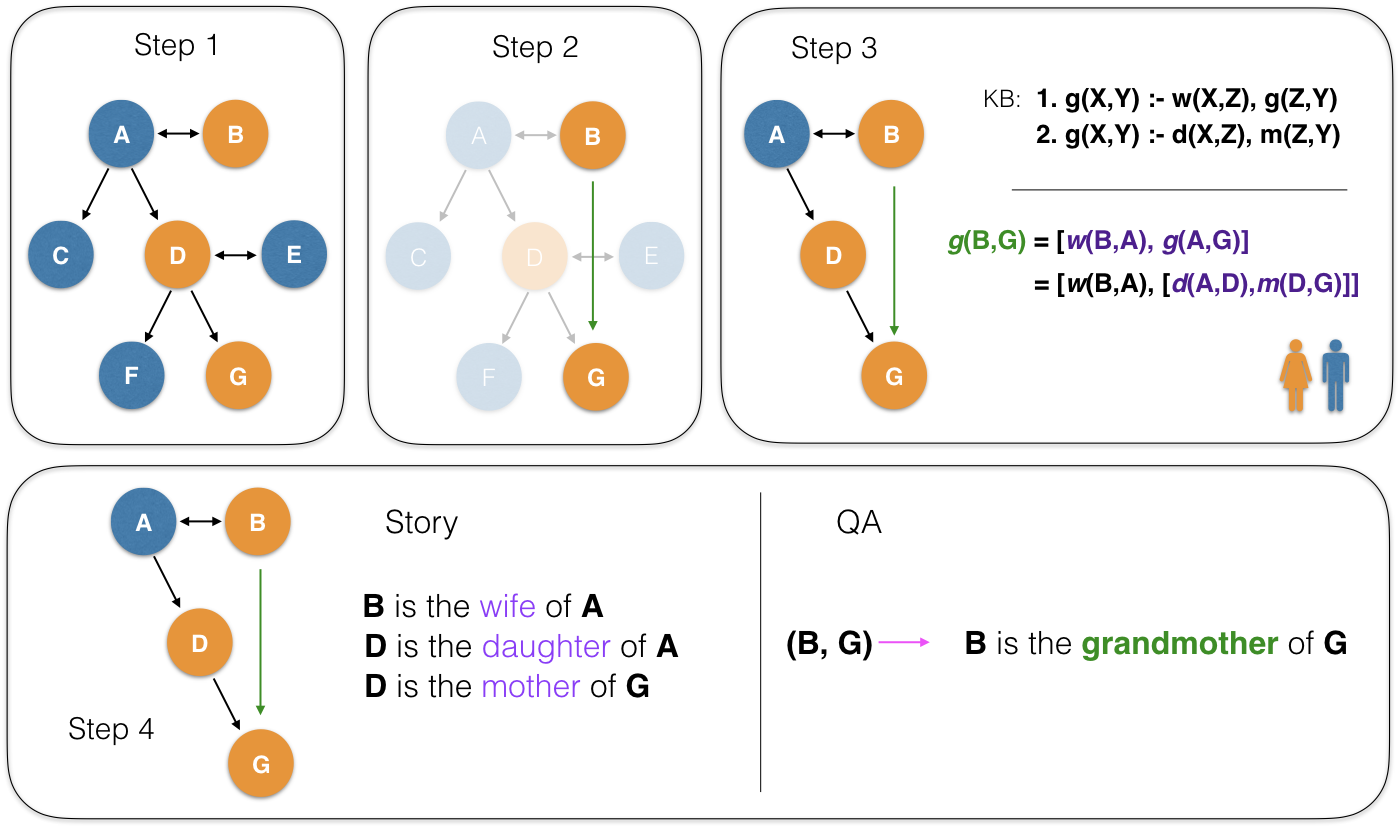
\includegraphics[]{figs/clutrr/dataset_const_new.png}}
\caption{Data generation pipeline. Step 1: generate a kinship graph. Step 2: sample a target fact. Step 3: Use backward chaining to sample a set of facts. Step 4: Convert sampled facts to a natural language story.}
\label{fig:clutrr:data}
\end{figure}


The core idea behind the CLUTRR benchmark suite is the following: Given a natural language story describing a set of kinship relations, the goal is to infer the relationship between two entities, whose relationship is {\em not} explicitly stated in the story.
To generate these stories, we first design a knowledge base (KB) with rules specifying how kinship relations resolve, and we use the following steps to create semi-synthetic stories based on this knowledge base:
\begin{enumerate}[topsep=3pt, parsep=6pt, leftmargin=40pt, itemsep=0pt, label={\bf Step \arabic*.}]
    \item \textbf{Generate} a random kinship graph that satisfies the rules in our KB.
    \item
        \textbf{Sample a target fact} (i.e., relation) to predict from the kinship graph.
    \item
        \textbf{Apply backward chaining} to sample a set of facts that can prove the target relation (and optionally sample a set of ``distracting'' or ``irrelevant'' noise facts).
    \item
        \textbf{Convert the sampled facts into a natural language story} through pre-specified text templates and crowd-sourced paraphrasing.
\end{enumerate}

Figure \ref{fig:clutrr:data} provides a high-level overview of this idea, and the following subsections describe the data generation process in detail, as well as the diagnostic flexibility afforded by CLUTRR.


% \subsection{Dataset construction}
% \label{sec:clutrr_data_const}

The short stories in CLUTRR are essentially narrativized renderings of a set of logical facts.
In the following sections, we describe how we sample the logical facts that make up a story by generating random kinship graphs and using backward chaining to produce logical reasoning chains.

% \subsection{Terminology and background}

\subsection{Graph generation}

%We restrict the set of rules in $R$ to consist of two atoms in the body (see the Appendix for the full set of rules).
% Using the logical rules in $R$ (see the Appendix for the full set of rules), we build a \textit{clause} which can be a conjunction of one or multiple rules.  %Further, we consider only binary predicates that make it easy to define a graph structure on the story.

To generate a kinship graph (say, $G$) underlying a particular story, we first sample a set of gendered\footnote{Kinship and gender roles are oversimplified in our data (compared to the real world) to maintain tractability.} entities and kinship relations using a stochastic generation process.
This generation process contains a number of tunable parameters---such as the maximum number of children at each node, the probability of an entity being married to another entity, etc.---and is designed to produce a valid, but possibly incomplete ``backbone graph''.
For instance, this backbone graph generation process will specify ``parent''/``child'' relations between entities but does not add ``grandparent'' relations.
After this initial generation process, we recursively apply the logical rules in $R$ to the backbone graph to produce a final graph $G$ that contains the full set of kinship relations between all the entities.
\footnote{In the context of our data generation process, we distinguish between the knowledge base, $R$, which contains a finite number of predicates and rules specifying how kinship relations in a family resolve, and a particular kinship graph $G$, which contains a grounded set of atoms specifying the particular kinship relations that underlie a single story.
In other words, $R$ contains the logical rules that govern all the generated stories in CLUTRR, while $G$ contains the grounded facts that underlie a specific story.}

In the CLUTRR Benchmark, the following kinship relations are used: \textit{son, father, husband, brother, grandson, grandfather, son-in-law, father-in-law, brother-in-law, uncle, nephew, daughter, mother, wife, sister, granddaughter, grandmother, daughter-in-law, mother-in-law, sister-in-law, aunt, niece}.

\footnotesize
\begin{align*}
\begin{split}
    [\texttt{grand}, X,Y] &\vdash [[\texttt{child}, X,Z],[\texttt{child}, Z,Y]], \\
    [\texttt{grand}, X,Y] &\vdash [[\texttt{SO}, X,Z],[\texttt{grand}, Z,Y]], \\
    [\texttt{grand}, X,Y] &\vdash [[\texttt{grand}, X,Z], [\texttt{sibling}, Z,Y]], \\
    [\texttt{inv-grand}, X,Y] &\vdash [[\texttt{inv-child}, X,Z], [\texttt{inv-child}, Z,Y]], \\
    [\texttt{inv-grand}, X,Y] &\vdash [[\texttt{sibling}, X,Z], [\texttt{inv-grand}, Z,Y]], \\
    [\texttt{child}, X,Y] &\vdash [[\texttt{child}, X,Z], [\texttt{sibling}, Z,Y]], \\
  [\texttt{child}, X,Y] &\vdash [[\texttt{SO}, X,Z], [\texttt{child}, Z,Y]], \\
  [\texttt{inv-child}, X,Y] &\vdash [[\texttt{sibling}, X,Z], [\texttt{inv-child}, Z,Y]], \\
    [\texttt{inv-child}, X,Y] &\vdash [[\texttt{child}, X,Z], [\texttt{inv-grand}, Z,Y]], \\
    [\texttt{sibling}, X,Y] &\vdash [[\texttt{child}, X,Z], [\texttt{inv-un}, Z,Y]], \\
    [\texttt{sibling}, X,Y] &\vdash [[\texttt{inv-child}, X,Z], [\texttt{child}, Z,Y]] \\
    [\texttt{sibling}, X,Y] &\vdash [[\texttt{sibling}, X,Z],[\texttt{sibling}, Z,Y]], \\
    [\texttt{in-law}, X,Y] &\vdash [[\texttt{child}, X,Z],[\texttt{SO}, Z,Y]], \\
    [\texttt{inv-in-law}, X,Y] &\vdash [[\texttt{SO}, X,Z],[\texttt{inv-child}, Z,Y]], \\
    [\texttt{un}, X,Y] &\vdash [[\texttt{sibling}, X,Z],[\texttt{child}, Z,Y]], \\
    [\texttt{inv-un}, X,Y] &\vdash [[\texttt{inv-child}, X,Z],[\texttt{sibling}, Z,Y]], \\
\end{split}
\end{align*}
\normalsize


We used a small, tractable, and logically sound KB of rules as mentioned above. We carefully select this set of deterministic rules to avoid ambiguity in the resolution. We use gender-neutral predicates and resolve the gender of the predicate in the head $\mathcal{H}$ of a clause $\mathcal{C}$ by deducing the gender of the second constant. We have two types of predicates, \textit{vertical} predicates (parent-child relations) and  \textit{horizontal} predicates (sibling or significant other). We denote all the vertical predicates by its \textit{child-to-parent} relation and append the prefix \texttt{inv-} to the predicates for the corresponding \textit{parent-to-child} relation. For example, \texttt{grandfatherOf} is denoted by the gender-neutral predicate $[\texttt{inv-grand},X,Y]$, where the gender is determined by the gender of $Y$.



\subsection{Backward chaining}
The resulting graph $G$ provides the \textit{background knowledge} for a specific story, as each edge in this graph can be treated as a grounded predicate (i.e., fact) between two entities.
From this graph $G$, we sample the facts that make up the story, as well as the target fact that we seek to predict:
First, we (uniformly) sample a target relation $\mathcal{H}_{\mathcal{C}}$, which is the fact that we want to predict from the story.
Then, from this target relation $\mathcal{H}_{\mathcal{C}}$,  we run a simple variation of the backward chaining \citep{gallaire1978logic} algorithm for $k$ iterations starting from $\mathcal{H}_{\mathcal{C}}$, where at each iteration we uniformly sample a subgoal to resolve and then uniformly sample a KB rule that resolves this subgoal.
Crucially, unlike traditional backward chaining, we do not stop the algorithm when a proof is obtained; instead, we run for a fixed number of iterations $k$ in order to sample a set of $k$ facts $\mathcal{B}_{\mathcal{C}}$ that imply the target relation $\mathcal{H}_{\mathcal{C}}$.

\subsection{Adding natural language}
\label{subsec:clutrr_nat_lang}

So far, we have described the process of generating a  conjunctive logical clause $\mathcal{C}=(\mathcal{H}_{\mathcal{C}} \vdash \mathcal{B}_{\mathcal{C}})$, where $\mathcal{H}_{\mathcal{C}}=[\alpha^*]$ is the target fact (i.e., relation) we seek to predict and $\mathcal{B}_{\mathcal{C}} = [\alpha_1, ..., \alpha_k]$ is the set of supporting facts that imply the target relation.
We now describe how we convert this logical representation to natural language through crowd-sourcing.

\subsubsection{Paraphrasing using Amazon Mechanical Turk}

We use Amazon Mechanical Turk (AMT), an online platform for collecting annotations from crowd-workers \footnote{\href{https://www.mturk.com/}{https://www.mturk.com/}}. The platform supports a mechanism to quickly annotate large amounts of data by paying anonymous workers for their effort. In our work, the crowd-workers are shown a set of facts $\mathcal{B}_{\mathcal{C}}$ corresponding to a story and then they are asked to paraphrase these facts into a narrative.
Since workers are given a set of facts $\mathcal{B}_{\mathcal{C}}$ to work from, they are able to combine and split multiple facts across separate sentences and construct diverse narratives (Figure \ref{fig:clutrr:lang_composition}).

We use ParlAI \citep{miller2017parlai} Mturk interface to collect paraphrases from the users. Specifically, given a set of facts, we ask the users to paraphrase the facts into a story. The users (\textit{turkers}) are free to construct any story they like as long as they mention all the entities and all the relations among them. We also provide the head $\mathcal{H}$ of the clause as an \textit{inferred} relation and specifically instruct the users to \textit{not} mention it in the paraphrased story. In order to evaluate the paraphrased stories, we ask the turkers to peer review a story paraphrased by a different turker. Since there are two tasks - paraphrasing a story and rating a story - we choose to pay 0.5\$ for each annotation. A sample task description in our MTurk interface is as follows:

\begin{quote}\small
    In this task, you will need to write a short, simple story based on a few facts. \textbf{It is crucial that the story mentions each of the given facts at least once.} The story does not need to be complicated! It just needs to be grammatical and mention the required facts.

    After writing the story, you will be asked to evaluate the quality of a generated story (based on a different set of facts). \textbf{It is crucial that you check whether the generated story mentions each of the required facts.}

    \textit{Example of good and bad stories: Good Example}

    \textbf{Facts to Mention}
    \begin{itemize}
        \item John is the father of Sylvia.
        \item Sylvia has a brother Patrick.
    \end{itemize}

    \textbf{Implied Fact}: John is the father of Patrick.

    \textbf{Written story}

    John is the proud father of the lovely Sylvia. Sylvia has a love-hate relationship with her brother Patrick.

    \textit{Bad Example}

    \textbf{Facts to Mention}

    \begin{itemize}
        \item Vincent is the son of Tim.
        \item Martha is the wife of Tim.
    \end{itemize}

    \textbf{Implied Fact} : Martha is Vincent's mother.

    \textbf{Written story}

    Vincent is married at Tim and his mother is Martha.

    \textit{The reason the above story is bad}:

    \begin{itemize}
        \item This story is bad because it is nonsense / ungrammatical.
        \item This story is bad because it does not mention the proper facts.
        \item This story is bad because it reveals the implied fact.
    \end{itemize}
\end{quote}

A sample of the AMT interface is shown in \autoref{fig:clutrr:mturk}.
To ensure that the turkers are providing high-quality annotations without revealing the inferred fact, we also launch another task to ask the turkers to rate three annotations to be either good or bad which are provided by a set of \textit{different} turkers. We pay 0.2\$ for each HIT consisting of three reviews. This helped to remove logical and grammatical inconsistencies to a large extent. Based on the reviews, 79\% of the collected paraphrases passed the peer-review sanity check where all the reviewers agree on the quality. This subset of the placeholders is used in the benchmark. A sample of programmatically generated dataset for clause length of $k=2$ to $k=6$ is provided in the tables \ref{tab:puzzle_data_1} to \ref{tab:puzzle_data_5}.

\begin{figure*}[h]
  \centering
  \resizebox{0.8\textwidth}{!}{
    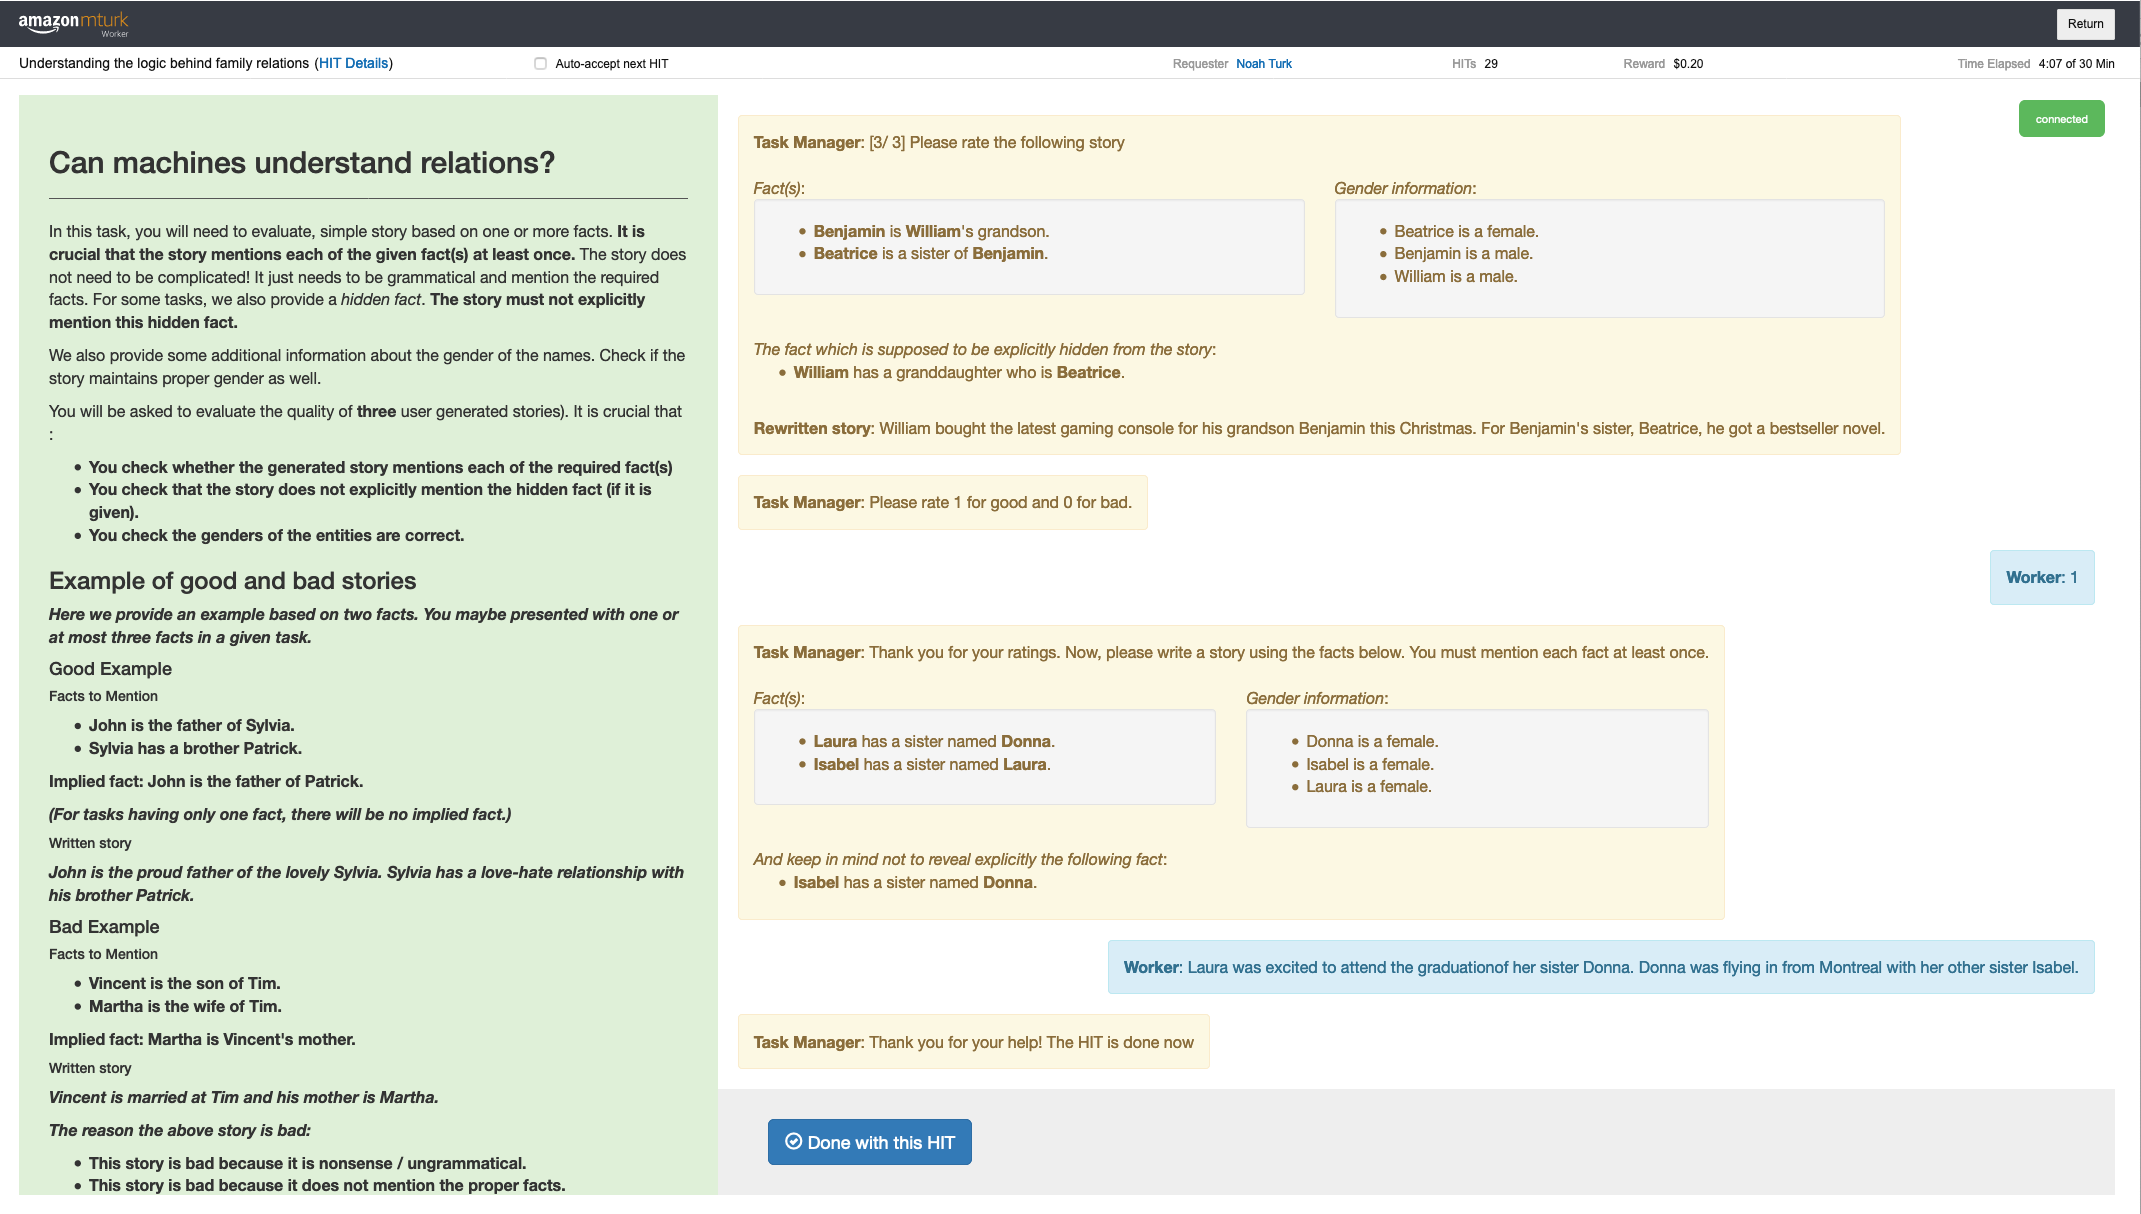
\includegraphics[width=\textwidth]{figs/clutrr/mturk_interface.png}}
    \caption{Amazon Mechanical Turker Interface built using ParlAI which was used to collect data as well as peer reviews.}%
    \label{fig:clutrr:mturk}
\end{figure*}



\subsubsection{Reusability and composition}
One challenge for data collection via AMT is that the number of possible stories generated by CLUTRR grows combinatorially as the number of supporting facts increases, i.e., as  $k=|\mathcal{B}_{\mathcal{C}}|$ grows.
This combinatorial explosion for large $k$---combined with the difficulty of maintaining the quality of the crowd-sourced paraphrasing for long stories---makes it infeasible to obtain a large number of paraphrased examples for $k>3$.
To circumvent this issue and increase the flexibility of our benchmark, we reuse and compose AMT paraphrases to generate longer stories.
In particular, we collected paraphrases for stories containing $k=1,2,3$ supporting facts and then replaced the entities from these collected stories with placeholders in order to re-use them to generate longer semi-synthetic stories.
An example of a story generated by stitching together two shorter paraphrases is provided below:
\vspace{-5pt}
\begin{quote}{\small
    [Frank] went to the park with his father, [Brett]. [Frank] called his brother [Boyd] on the phone. He wanted to go out for some beers.
    [Boyd] went to the baseball game with his son [Jim].\\
    Q: What is [Brett] and [Jim]'s relationship?}
\end{quote}
\vspace{-5pt}
Thus, instead of simply collecting paraphrases for a fixed number of stories, we instead obtain a diverse collection of natural language templates that can be programmatically recombined to generate stories with various properties.

\subsection{AMT Template statistics}


\begin{table}[]
\centering
\resizebox{0.48\textwidth}{!}{%
\begin{tabular}{@{}rrll@{}}
\toprule
\multicolumn{1}{l}{Number of Paraphrases} & \multicolumn{1}{l}{} &  & \# clauses \\ \midrule
\multicolumn{1}{r|}{} & $k$ = 1 & 1,868 & \multicolumn{1}{c}{20} \\
\multicolumn{1}{r|}{} & $k$ = 2 & 1,890 & \multicolumn{1}{c}{58} \\
\multicolumn{1}{r|}{} & $k$ = 3 & 2,258 & \multicolumn{1}{c}{236} \\ \cmidrule(l){2-4} 
\multicolumn{1}{r|}{} & Total & 6,016 &  \\ \midrule
\multicolumn{1}{l}{Unique Word Count} &  & 3,797 &  \\ \midrule
\multicolumn{1}{r|}{Jaccard Word Overlap} & Unigrams & 0.201 &  \\
\multicolumn{1}{r|}{} & Bigrams & 0.0385 &  \\ \bottomrule
\end{tabular}%
}
\caption{Statistics of the AMT paraphrases. Jaccard word overlap is calculated within the templates of each individual clause of length $k$.}
\label{tab:placeholder}
\end{table}


At the time of submission, we have collected 6,016 unique paraphrases with an average of 19 paraphrases for every possible logical clause of length $k=1,2,3$. Table \ref{tab:placeholder} contains summary statistics of the collected paraphrases.
Overall, we found high linguistic diversity in the collected paraphrases.
For instance, the average Jaccard overlap in unigrams between pairs paraphrases corresponding to the same logical clause was only 0.201 and only 0.0385 for bigrams.

\subsection{Human performance}

% Please add the following required packages to your document preamble:
% \usepackage{booktabs}
% \usepackage{multirow}
% \usepackage{graphicx}
\begin{table}[]
\centering
\resizebox{0.7\textwidth}{!}{%
\begin{tabular}{@{}llll@{}}
\toprule
\multirow{2}{*}{Relation Length} & \multicolumn{2}{l}{Human Performance} & \multirow{2}{*}{Reported Difficulty} \\
 & Time Limited & Unlimited Time &  \\ \midrule
2 & 0.848 & 1 & 1.488 +- 1.25 \\
3 & 0.773 & 1 & 2.41 +- 1.33 \\
4 & 0.477 & 1 & 3.81 +- 1.46 \\
5 & 0.424 & 1 & 3.78 +- 0.96 \\
6 & 0.406 & 1 & 4.46 +- 0.87 \\ \bottomrule
\end{tabular}%
}
\caption{Human performance accuracies on CLUTRR dataset. Humans are provided the Clean-Generalization version of the dataset, and we test on two scenarios: when a human is given limited time to solve the task, and when a human is given unlimited time to solve the task. Regardless of time, our evaluators provide a score of difficulty of individual puzzles.}
\label{tab:clutrr:human_perf}
\end{table}


To get a sense of the data quality and difficulty involved in CLUTRR, we asked human annotators to solve the task for random examples of length $k=2,3,...,6$. (\autoref{tab:clutrr:human_perf})
We perform the evaluation in two scenarios: first a time-limited scenario where we ask AMT Turkers to solve the puzzle in a fixed time. Turkers were provided a maximum time of 30 mins, but they solved the puzzles in an average of 1 minute 23 seconds. Secondly, we use another set of expert evaluators who are given ample time to solve the tasks. Not surprisingly, if a human being is given ample time (experts took an average of 6 minutes per puzzle) and a pen and a paper to aid in the reasoning, they get all the relations correct. However, if an evaluator is short of time, they might miss important details on the relations and perform poorly. Thus, our tasks require \textit{active attention}.

We found that time-constrained AMT annotators performed well (i.e., ${>70\%}$) accuracy for ${k\leq 3}$ but struggled with examples involving longer stories, achieving 40-50\% accuracy for ${k > 3}$. However, trained annotators with unlimited time were able to solve 100\% of the examples, highlighting the fact that this task requires attention and involved reasoning, even for humans.

\subsection{Representing the question and entities}

The AMT paraphrasing approach described above allows us to convert the set of supporting facts $\mathcal{B}_{\mathcal{C}}$ to a natural language story, which can be used to predict the target relation/query $\mathcal{H}_{\mathcal{C}}$.
However, instead of converting the target query, $\mathcal{H}_{\mathcal{C}} = [\alpha^*]$, to a natural language question, we instead opt to represent the target query as a $K$-way classification task, where the two entities in the target relation are provided as input and the goal is to classify the relation that holds between these two entities.
This representation avoids the pitfall of revealing information about the answer in the question \citep{kaushik2018much}.

When generating stories, entity names are randomly drawn from a set of 300 common gendered English names.
Thus, depending on each run, the entities are never the same.
This ensures that the entity names are simply placeholders and uncorrelated from the task.



\begin{figure}[t]
\centering
\resizebox{0.45\textwidth}{!}{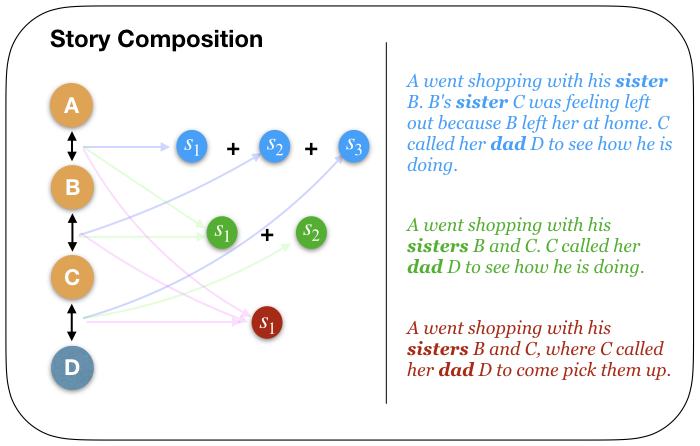
\includegraphics[]{figs/clutrr/composition.png}}
\caption{Illustration of how a set of facts can split and combined in various ways across sentences.}
\label{fig:clutrr:lang_composition}
\end{figure}


\begin{figure}[t]
\centering
\resizebox{0.38\textwidth}{!}{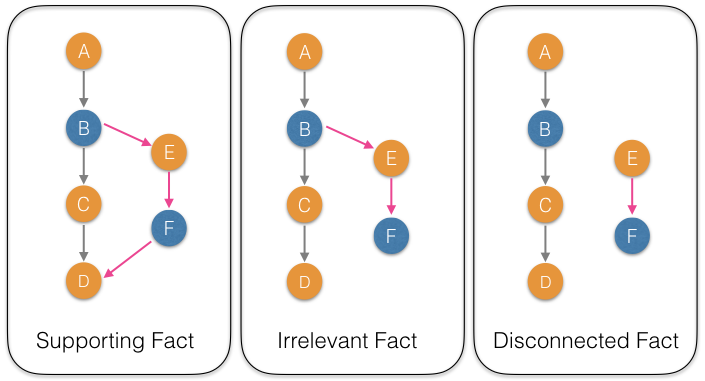
\includegraphics[]{figs/clutrr/clutrr_noise.png}}
\caption{Noise generation procedures of CLUTRR.}
\label{fig:clutrr:data_noise}
\end{figure}



\section{Experimental Setups}
\label{sec:clutrr_setups}

The modular nature of CLUTRR provides rich diagnostic capabilities for evaluating the robustness and generalization abilities of neural language understanding systems.
We highlight some key diagnostic capabilities available via different variations of CLUTRR below.
These diagnostic variations correspond to the concrete datasets that we generated in this work, and we describe the results on these datasets in \autoref{sec:clutrr_results}.

\subsection{Systematic generalization}

Most prominently, CLUTRR allows us to explicitly evaluate a model's ability for generalizing with the property of systematicity.
In particular, we rely on the following hold-out procedures to test systematic generalization:
\begin{itemize}[leftmargin=*, topsep=2pt, itemsep=2pt, parsep=2pt]
    \item During training, we hold out a subset of the collected paraphrases, and we only use this held-out subset of paraphrases when generating the test set.
    Thus, to succeed on CLUTRR, an NLU system must exhibit {\em linguistic generalization} and be robust to linguistic variation at test time.
    \item We also hold out a subset of the logical clauses during training (for clauses of length $k > 2$).\footnote{One should not holdout clauses from length $k=2$ in order to allow models to learn the compositionality of all possible binary predicates.}
    In other words, during training, the model sees all logical rules but does not see all {\em combinations} of these logical rules.
    Thus, in addition to linguistic generalization, success on this task also requires {\em logical generalization}.
    \item
    Lastly, as a more extreme form of both logical and linguistic generalization, we consider the setting where the models are trained on stories generated from clauses of length ${\leq k}$ and evaluated on stories generated from larger clauses of length ${>k}$. Thus, we explicitly test the ability for models to generalize on examples that require more steps of reasoning that any example they encountered during training.
\end{itemize}

\subsection{Robust Reasoning}
\label{sec:clutrr_robust_data}

In addition to evaluating systematic generalization, the modular setup of CLUTRR also allows us to diagnose model robustness by adding \textit{noise facts} to the generated narratives.
Due to the controlled semi-synthetic nature of CLUTRR, we are able to provide a precise taxonomy of the kinds of noise facts that can be added (Figure \ref{fig:clutrr:data_noise}).
In order to structure this taxonomy, it is important to recall that any set of supporting facts $\mathcal{B}_{\mathcal{C}}$ generated by CLUTRR can be interpreted as a path, $p_{\mathcal{C}}$, in the corresponding kinship graph $G$ (Figure \ref{fig:clutrr:data}).
Based on this interpretation, we view adding noise facts from the perspective of sampling three different types of noise paths, $p_n$, from the kinship graph $G$:
\begin{itemize}[  leftmargin=10pt, topsep=0pt, itemsep=0pt, parsep=0pt]
    \item \textit{Irrelevant facts}: We add a path $p_n$, which has exactly one shared end-point with $p_c$. In this way, this is a \textit{distractor} path,
    which contains facts that are connected to one of the entities in the target relation, $\mathcal{H}_{\mathcal{C}}$, but do not provide any information that could be used to help answer the query. %We name this task \texttt{CLUTRR-Irrelevant}
     \item \textit{Supporting facts}:
    We add a path $p_n$, whose two end-points are on the path $p_{\mathcal{C}}$.
    The facts on this path $p_n$ are noise because they are not needed to answer the query, but they are supporting facts because they can, in principle, be used to construct alternative (longer) reasoning paths that connect the two target entities.
    %We denote this setup as \texttt{CLUTRR-Supporting}
    \item \textit{Disconnected facts}: We add paths which neither originate nor end in any entity on $p_c$. These disconnected facts involve entities and relations that are completely unrelated to the target query.
    %We call this variant \texttt{CLUTRR-Disconnected}.
\end{itemize}

\subsection{Generated Datasets}

For all experiments, we generated datasets with 10-15k training examples.
In many experiments, we report training and testing results on stories with different clause lengths $k$.
(For brevity, we use the phrase ``clause length'' throughout this section to refer to the value $k=|\mathcal{B}_{\mathcal{C}}|$, i.e., the number of steps of reasoning that are required to predict the target query.)
In all cases, the training set contains 5000 train stories per $k$ value, and, during testing, all experiments use 100 test stories per $k$ value.
All experiments were run 10 times with different randomly generated stories, and means and standard errors over these 10 runs are reported.
As discussed above, during training we holdout 20\% of the paraphrases, as well as 10\% of the possible logical clauses.


% Please add the following required packages to your document preamble:
% \usepackage{booktabs}
% \usepackage{graphicx}
\begin{table*}[]
\centering
\caption{Snapshot of puzzles in the dataset for k=2}
\label{tab:puzzle_data_1}
\resizebox{0.7\textwidth}{!}{%
\begin{tabular}{@{}p{7cm}lll@{}}
\toprule
\textbf{Puzzle} & \textbf{Question} & \textbf{Gender} & \textbf{Answer} \\ \midrule
\addlinespace[0.5em]
\noindent\parbox[c]{\hsize}{\textit{Charles}'s son \textit{Christopher} entered rehab for the ninth time at the age of thirty. \textit{Randolph} had a nephew called \textit{Christopher} who had n't seen for a number of years.} & Randolph is the \_\_\_\_\_ of Charles & \begin{tabular}[c]{@{}l@{}}Charles:male,\\ Christopher:male,\\ Randolph:male\end{tabular} & brother \\
\addlinespace[0.5em]
\noindent\parbox[c]{\hsize}{\textit{Randolph} and his sister \textit{Sharon} went to the park. \textit{Arthur} went to the baseball game with his son \textit{Randolph}}. & Sharon is the \_\_\_\_\_ of Arthur & \begin{tabular}[c]{@{}l@{}}Arthur:male,\\ Randolph:male,\\ Sharon:female\end{tabular} & daughter \\
\addlinespace[0.5em]
\noindent\parbox[c]{\hsize}{\textit{Frank} went to the park with his father, \textit{Brett}. \textit{Frank} called his brother \textit{Boyd} on the phone. He wanted to go out for some beers.} & Brett is the \_\_\_\_\_ of Boyd & \begin{tabular}[c]{@{}l@{}}Boyd:male,\\ Frank:male,\\ Brett:male\end{tabular} & father \\ \bottomrule
\end{tabular}%
}
\end{table*}

% Please add the following required packages to your document preamble:
% \usepackage{booktabs}
% \usepackage{graphicx}
\begin{table*}[]
\centering
\caption{Snapshot of puzzles in the dataset for k=3}
\label{tab:puzzle_data_2}
\resizebox{0.7\textwidth}{!}{%
\begin{tabular}{@{}p{7cm}lll@{}}
\toprule
\textbf{Puzzle} & \textbf{Question} & \textbf{Gender} & \textbf{Answer} \\ \midrule
\textit{Roger} was playing baseball with his sons \textit{Sam} and \textit{Leon}. \textit{Sam} had to take a break though because he needed to call his sister \textit{Robin}. & Leon is the \_\_\_\_\_ of Robin & \begin{tabular}[c]{@{}l@{}}Robin:female,\\ Sam:male,\\ Roger:male,\\ Leon:male\end{tabular} & brother \\
\textit{Elvira} and her daughter \textit{Nancy} went shopping together last Monday and they bought new shoes for \textit{Elvira}'s kids. \textit{Pedro} and his sister \textit{Allison} went to the fair. \textit{Pedro}'s mother, \textit{Nancy}, was out with friends for the day. & Elvira is the \_\_\_\_\_ of Allison & \begin{tabular}[c]{@{}l@{}}Allison:female,\\ Pedro:male,\\ Nancy:female,\\ Elvira:female\end{tabular} & grandmother \\
\textit{Roger} met up with his sister \textit{Nancy} and her daughter \textit{Cynthia} at the mall to go shopping together. \textit{Cynthia}'s brother \textit{Pedro} was going to be the star in the new show. & Pedro is the \_\_\_\_\_ of Roger & \begin{tabular}[c]{@{}l@{}}Roger:male,\\ Nancy:female,\\ Cynthia:female,\\ Pedro:male\end{tabular} & nephew \\ \bottomrule
\end{tabular}%
}
\end{table*}

% Please add the following required packages to your document preamble:
% \usepackage{booktabs}
% \usepackage{graphicx}
\begin{table*}[]
\centering
\caption{Snapshot of puzzles in the dataset for k=4}
\label{tab:puzzle_data_3}
\resizebox{0.7\textwidth}{!}{%
\begin{tabular}{@{}p{7cm}lll@{}}
\toprule
\textbf{Puzzle} & \textbf{Question} & \textbf{Gender} & \textbf{Answer} \\ \midrule
\textit{Celina} has been visiting her sister, \textit{Fran} all week. \textit{Fran} is also the daughter of \textit{Bethany}. \textit{Ronald} loves visiting his aunt \textit{Bethany} over the weekends. \textit{Samuel}'s son \textit{Ronald} entered rehab for the ninth time at the age of thirty. & Celina is the \_\_\_\_\_ of Samuel & \begin{tabular}[c]{@{}l@{}}Samuel:male,\\ Ronald:male,\\ Bethany:female,\\ Fran:female,\\ Celina:female\end{tabular} & niece \\
\textit{Celina} adores her daughter \textit{Bethany}. \textit{Bethany} loves her very much, too. \textit{Jackie} called her mother \textit{Bethany} to let her know she will be back home soon. \textit{Thomas} was helping his daughter \textit{Fran} with her homework at home. Afterwards, \textit{Fran} and her sister \textit{Jackie} played Xbox together. & Celina is the \_\_\_\_\_ of Thomas & \begin{tabular}[c]{@{}l@{}}Thomas:male,\\ Fran:female,\\ Jackie:female,\\ Bethany:female,\\ Celina:female\end{tabular} & daughter \\
\textit{Raquel} is \textit{Samuel} 'daughter and they go shopping at least twice a week together. \textit{Kenneth} and her mom, \textit{Theresa}, had a big fight. \textit{Theresa}'s son, \textit{Ronald}, refused to get involved. \textit{Ronald} was having an argument with her sister, \textit{Raquel}. & Samuel is the \_\_\_\_\_ of Kenneth & \begin{tabular}[c]{@{}l@{}}Kenneth:male,\\ Theresa:female,\\ Ronald:male,\\ Raquel:female,\\ Samuel:male\end{tabular} & father \\ \bottomrule
\end{tabular}%
}
\end{table*}

% Please add the following required packages to your document preamble:
% \usepackage{booktabs}
% \usepackage{graphicx}
\begin{table*}[]
\centering
\caption{Snapshot of puzzles in the dataset for k=5}
\label{tab:puzzle_data_4}
\resizebox{0.7\textwidth}{!}{%
\begin{tabular}{@{}p{7cm}lll@{}}
\toprule
\textbf{Puzzle} & \textbf{Question} & \textbf{Gender} & \textbf{Answer} \\ \midrule
\textit{Steven}'s son is \textit{Bradford}. \textit{Bradford} and his father always go fishing together on Sundays and have a great time together. \textit{Diane} is taking her brother \textit{Brad} out for a late dinner. \textit{Kristin}, \textit{Brad}'s mother, is home with a cold. \textit{Diane}'s father \textit{Elmer}, and his brother \textit{Steven}, all got into the rental car to start the long cross-country roadtrip they had been planning. & Bradford is the \_\_\_\_\_ of Kristin & \begin{tabular}[c]{@{}l@{}}Kristin:female,\\ Brad:male,\\ Diane:female,\\ Elmer:male,\\ Steven:male,\\ Bradford:male\end{tabular} & nephew \\
\textit{Elmer} went on a roadtrip with his youngest child, \textit{Brad}. \textit{Lena} and her sister \textit{Diane} are going to a restaurant for lunch. \textit{Lena}'s brother \textit{Brad} is going to meet them there with his father \textit{Elmer} \textit{Brad} ca n't stand his unfriendly aunt \textit{Lizzie}. & Lizzie is the \_\_\_\_\_ of Diane & \begin{tabular}[c]{@{}l@{}}Diane:female,\\ Lena:female,\\ Brad:male,\\ Elmer:male,\\ Lizzie:female\end{tabular} & aunt \\
\textit{Ira} took his niece \textit{April} fishing Saturday. They caught a couple small fish. \textit{Ronald} was enjoying spending time with his parents, \textit{Damion} and \textit{Claudine}. \textit{Damion}'s other son, \textit{Dennis}, wanted to come visit too. \textit{Dennis} often goes out for lunch with his sister, \textit{April}. & Ira is the \_\_\_\_\_ of Claudine & \begin{tabular}[c]{@{}l@{}}Claudine:female,\\ Ronald:male,\\ Damion:male,\\ Dennis:male,\\ April:female,\\ Ira:male\end{tabular} & brother \\ \bottomrule
\end{tabular}%
}
\end{table*}

% Please add the following required packages to your document preamble:
% \usepackage{booktabs}
% \usepackage{graphicx}
\begin{table*}[]
\centering
\caption{Snapshot of puzzles in the dataset for k=6}
\label{tab:puzzle_data_5}
\resizebox{0.7\textwidth}{!}{%
\begin{tabular}{@{}p{7cm}lll@{}}
\toprule
\textbf{Puzzle} & \textbf{Question} & \textbf{Gender} & \textbf{Answer} \\ \midrule
\textit{Mario} wanted to get a good gift for his sister, \textit{Marianne}. \textit{Jean} and her sister \textit{Darlene} were going to a party held by \textit{Jean}'s mom, \textit{Marianne}. \textit{Darlene} invited her brother \textit{Roy} to come, too, but he was too busy. \textit{Teri} and her father, \textit{Mario}, had an argument over the weekend. However, they made up by Monday. \textit{Agnes} wants to make a special meal for her daughter \textit{Teri}'s birthday. & Roy is the \_\_\_\_\_ of Agnes & \begin{tabular}[c]{@{}l@{}}Agnes:female,\\ Teri:female,\\ Mario:male,\\ Marianne:female,\\ Jean:female,\\ Darlene:female,\\ Roy:male\end{tabular} & nephew \\
\textit{Robert}'s aunt, \textit{Marianne}, asked \textit{Robert} to mow the lawn for her. \textit{Robert} said he could n't because he had a bad back. \textit{William}'s parents, \textit{Brian} and \textit{Marianne}, threw him a surprise party for his birthday. \textit{Brian}'s daughter \textit{Jean} made a mental note to be out of town for her birthday! \textit{Agnes}'s biggest accomplishment is raising her son \textit{Robert}. \textit{Jean} is looking for a good gift for her sister \textit{Darlene}. & Darlene is the \_\_\_\_\_ of Agnes & \begin{tabular}[c]{@{}l@{}}Agnes:female,\\ Robert:male,\\ Marianne:female,\\ William:male,\\ Brian:male,\\ Jean:female,\\ Darlene:female\end{tabular} & niece \\
\textit{Sharon} and her brother \textit{Mario} went shopping. \textit{Teri}, \textit{Mario}'s daughter, came too. \textit{Agnes}, \textit{Annie}'s mother, is unhappy with \textit{Robert}. She feels her son is cruel to \textit{Annie}'s sister \textit{Teri}, and she wants \textit{Robert} to be nicer. \textit{Robert}'s sister, \textit{Nicole}, participated in the dance contest. & Nicole is the \_\_\_\_\_ of Sharon & \begin{tabular}[c]{@{}l@{}}Sharon:female,\\ Mario:male,\\ Teri:female,\\ Annie:female,\\ Agnes:female,\\ Robert:male,\\ Nicole:female\end{tabular} & niece \\ \bottomrule
\end{tabular}%
}
\end{table*}



\section{Evaluated Models}
\label{sec:clutrr_models}

Our primary baselines are neural language understanding models that take unstructured text as input.
We consider bidirectional LSTMs \citep{hochreiter1997long, cho2014learning} (with and without attention), as well as models that aim to incorporate inductive biases towards relational reasoning: Relation Networks (RN) \citep{santoro2017simple}, Relational Recurrent Networks (RMC) \citep{santoro2018relational} and Compositional Memory Attention Network (MAC) \citep{hudson2018compositional}. We also use the large pre-trained language model, BERT \citep{devlin2018bert}, as well as a modified version of BERT having a trainable LSTM encoder on top of the pretrained BERT embeddings.
All of these models (except BERT) were re-implemented in PyTorch 1.0 \citep{paszke2017automatic} and adapted to work with the CLUTRR benchmark.

Since the underlying relations in the stories generated by CLUTRR inherently form a graph, we also experiment with a Graph Attention Network (GAT) \citep{Velickovic2017-mh}.
%Specifically, we consider }, as a representative model from the field of graph representation learning \cite{2017arXiv170905584H}.
Rather than taking the textual stories as input, the GAT baseline receives a structured graph representation of the facts that underlie the story.
%The motivation behind the inclusion of the GAT baseline is to evaluate the difficulty of the inductive reasoning task without the challenge of interpreting the natural language.
%these two classes of models is to present the two extremes in current relational reasoning space : unstructured models which has to construct a latent graph, compared with structured model having the perfect graph as input.
%Future explorations can target the space between these models where an information retrieval (IR) model \citep{schoenmackers2010learning} can be used to extract the underlying graph from text and fed into a reasoning model.


\xhdr{Entity and query representations}
We use the various baseline models to encode the natural language story (or graph) into a fixed-dimensional embedding.
With the exception of the BERT models, we do not use pre-trained word embeddings and learn the word embeddings from scratch using end-to-end backpropagation.
An important note, however, is that we perform Cloze-style anonymization \citep{hermann2015teaching} of the entities (i.e., names) in the stories, where each entity name is replaced by a \textit{@entity-k} placeholder, which is randomly sampled from a small, fixed pool of placeholder tokens. The embeddings for these placeholders are randomly initialized and fixed during training.

To make a prediction about a target query given a story, we concatenate the embedding of the story (generated by the baseline model) with the embeddings of the two target entities and we feed this concatenated embedding to a 2-layer feed-forward neural network with a softmax prediction layer.

\subsection{Hyperparameters}

For all models, the common hyperparameters used are: Embedding dimension: 100 (except BERT based models), Optimizer: Adam, Learning rate: 0.001, Number of epochs: 100, Number of runs: 10. Specific model-based hyperparameters are given as follows:

\begin{itemize}
    \item \textbf{Bidirectional LSTM} \citep{hochreiter1997long, cho2014learning}: LSTM hidden dimension: 100, \# layers: 2, Classifier MLP hidden dimension: 200
    \item \textbf{Relation Networks} \citep{santoro2017simple}: $f_{{\theta}_1}$ : 256, $f_{{\theta}_2}$: 64, $g_{\theta}$ : 64
    \item \textbf{Compositional Memory Attention Network (MAC)} \citep{hudson2018compositional}: \# Iterations: 6, \texttt{shareQuestion}: True, Dropout - Memory, Read and Write: 0.2
    \item \textbf{Relational Recurrent Networks} \citep{santoro2018relational}: Memory slots: 2, Head size: 192, Number of heads: 4, Number of blocks : 1, forget bias : 1, input bias: 0, gate style: unit, key size: 64, \# Attention layers: 3, Dropout: 0
    \item \textbf{BERT} \citep{devlin2018bert}: Layers : 12, Fixed pretrained embeddings from \\ \texttt{bert-base-uncased} using Pytorch HuggingFace BERT repository \footnote{\hyperlink{https://github.com/huggingface/pytorch-pretrained-BERT}{https://github.com/huggingface/pytorch-pretrained-BERT}}, Word dimension: 768, appended with a two-layer MLP for final prediction.
    \item \textbf{BERT-LSTM}: Same parameters as above, with a two-layer unidirectional LSTM encoder on top of BERT word embeddings.
    \item \textbf{GAT} \citep{Velickovic2017-mh}: Node dimension: 100, Message dimension: 100, Edge dimension: 20, number of rounds: 3
\end{itemize}



\section{Results}
\label{sec:clutrr_results}

We evaluate several \acrshort{nlu} systems on the proposed CLUTRR benchmark to surface the relative strengths and shortcomings of these models in the context of inductive reasoning and combinatorial generalization.\footnote{Code to reproduce all the results in this section are available at  \href{https://github.com/facebookresearch/clutrr/}{https://github.com/facebookresearch/clutrr/}.} We aim to answer the following key questions:
\begin{enumerate}[label=({\bf Q\arabic*}), leftmargin=28pt, topsep=0pt, itemsep=0pt, parsep=0pt]
\item How do state-of-the-art NLU models compare in terms of systematic generalization? Can these models generalize to stories with unseen combinations of logical rules?
 \item How does the performance of neural language understanding models compare to a graph neural network that has full access to graph structure underlying the stories?
    \item How robust are these models to the addition of noise facts to a given story?
\end{enumerate}

\subsection{Systematic Generalization}
\label{sec:clutrr_sys_gen}

We begin by using CLUTRR to evaluate the ability of the baseline models to perform systematic generalization (\textbf{Q1}).
In this setting, we consider two training regimes: in the first regime, we train all models with clauses of length $k=2,3$, and in the second regime, we train with clauses of length $k=2,3,4$.
We then test the generalization of these models on test clauses of length $k=2,...,10$.

Figure \ref{fig:gen_1} illustrates the performance of different models on this generalization task.
We observe that the GAT model is able to perform near-perfectly on the held-out logical clauses of length $k=3$, with the BERT-LSTM being the top-performer among the text-based models but still significantly below the GAT.
Not surprisingly, the performance of all models degrades monotonically as we increase the length of the test clauses, which highlights the challenge of ``zero-shot'' systematic generalization \cite{lake2017generalization, 2018arXiv181107017S}.
However, as expected, all models improve on their generalization performance when trained on $k=2,3,4$ rather than just $k=2,3$ (Figure \ref{fig:gen_1}, right). The GAT, in particular, achieves the biggest gain by this expanded training.

\begin{figure*}[!htb]
     \centering
    \subfloat{{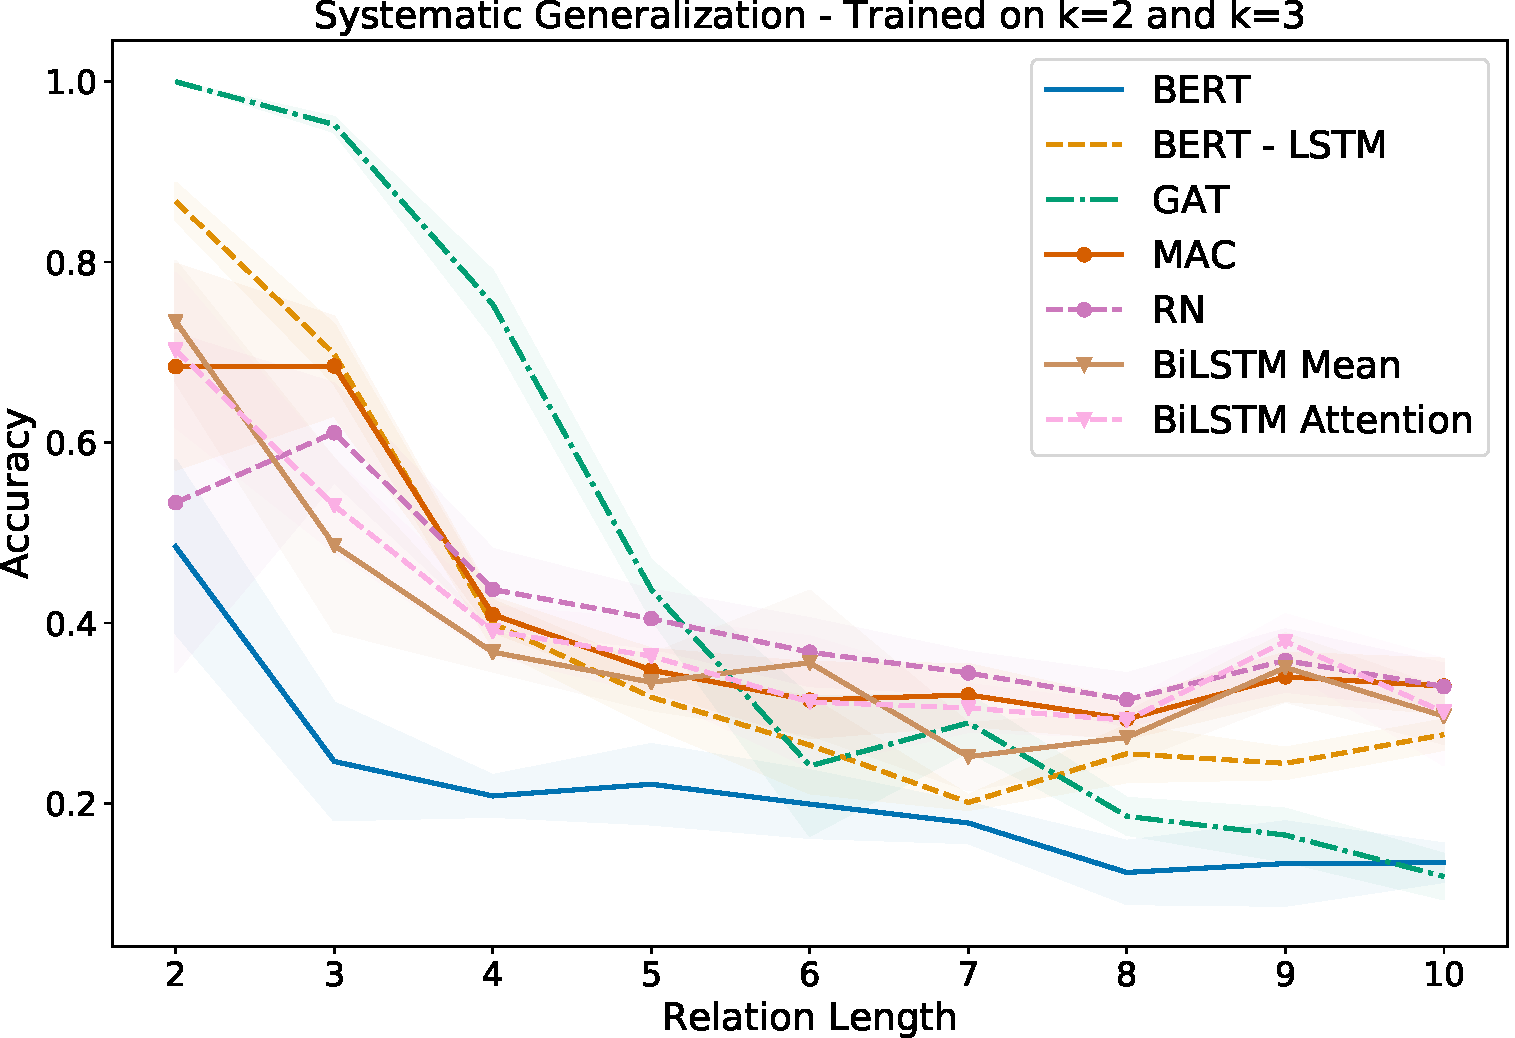
\includegraphics[width=0.48\textwidth]{figs/clutrr/emnlp/sys_gen_23.pdf} }}%
    \qquad
    \hspace{-20pt}
    \subfloat{{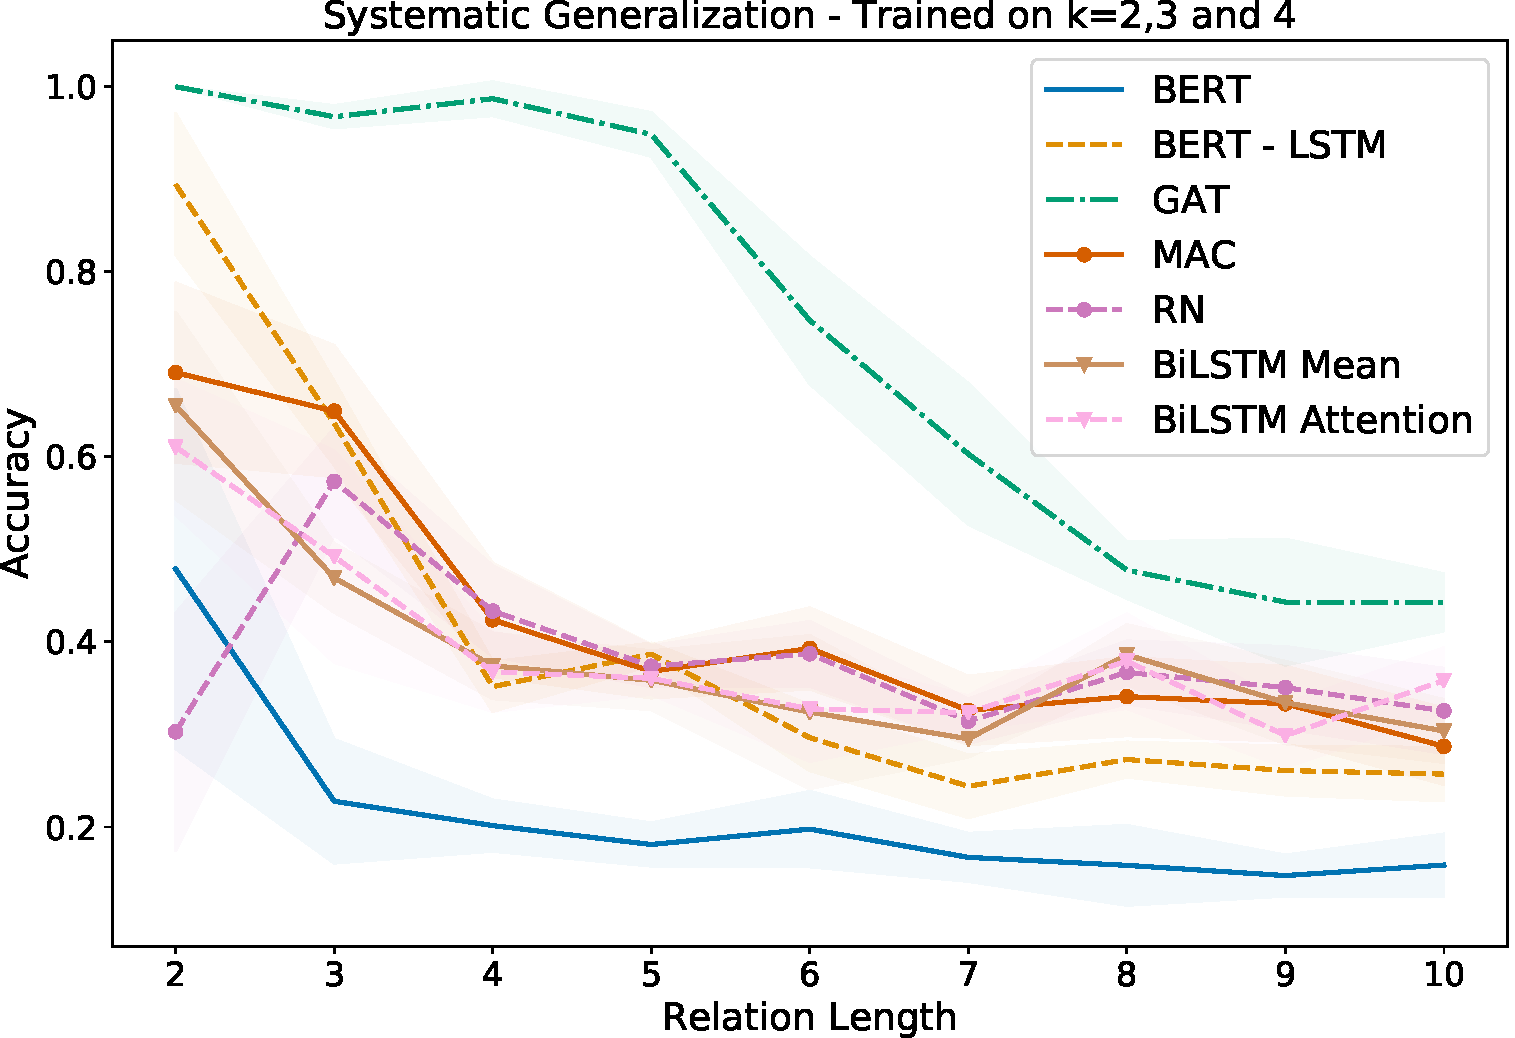
\includegraphics[width=0.48\textwidth]{figs/clutrr/emnlp/sys_gen_234.pdf} }}%
    \caption{Systematic generalization performance of different models when trained on clauses of length $k=2,3$ (Left) and $k=2,3,4$ (Right).}
    \label{fig:gen_1}
\end{figure*}



\subsection{The benefit of structure}
\label{sec:clutrr_structure}

The empirical results on systematic generalization also provide insight into how the text-based NLU systems compare against the graph-based GAT model that has full access to the logical graph structure underlying the stories (\textbf{Q2}).
Indeed, the relatively strong performance of the GAT model (Figure \ref{fig:gen_1}) suggests that the language-based models fail to learn a robust mapping from the natural language narratives to the underlying logical facts.

\begin{figure*}[!ht]
     \centering
    \subfloat{{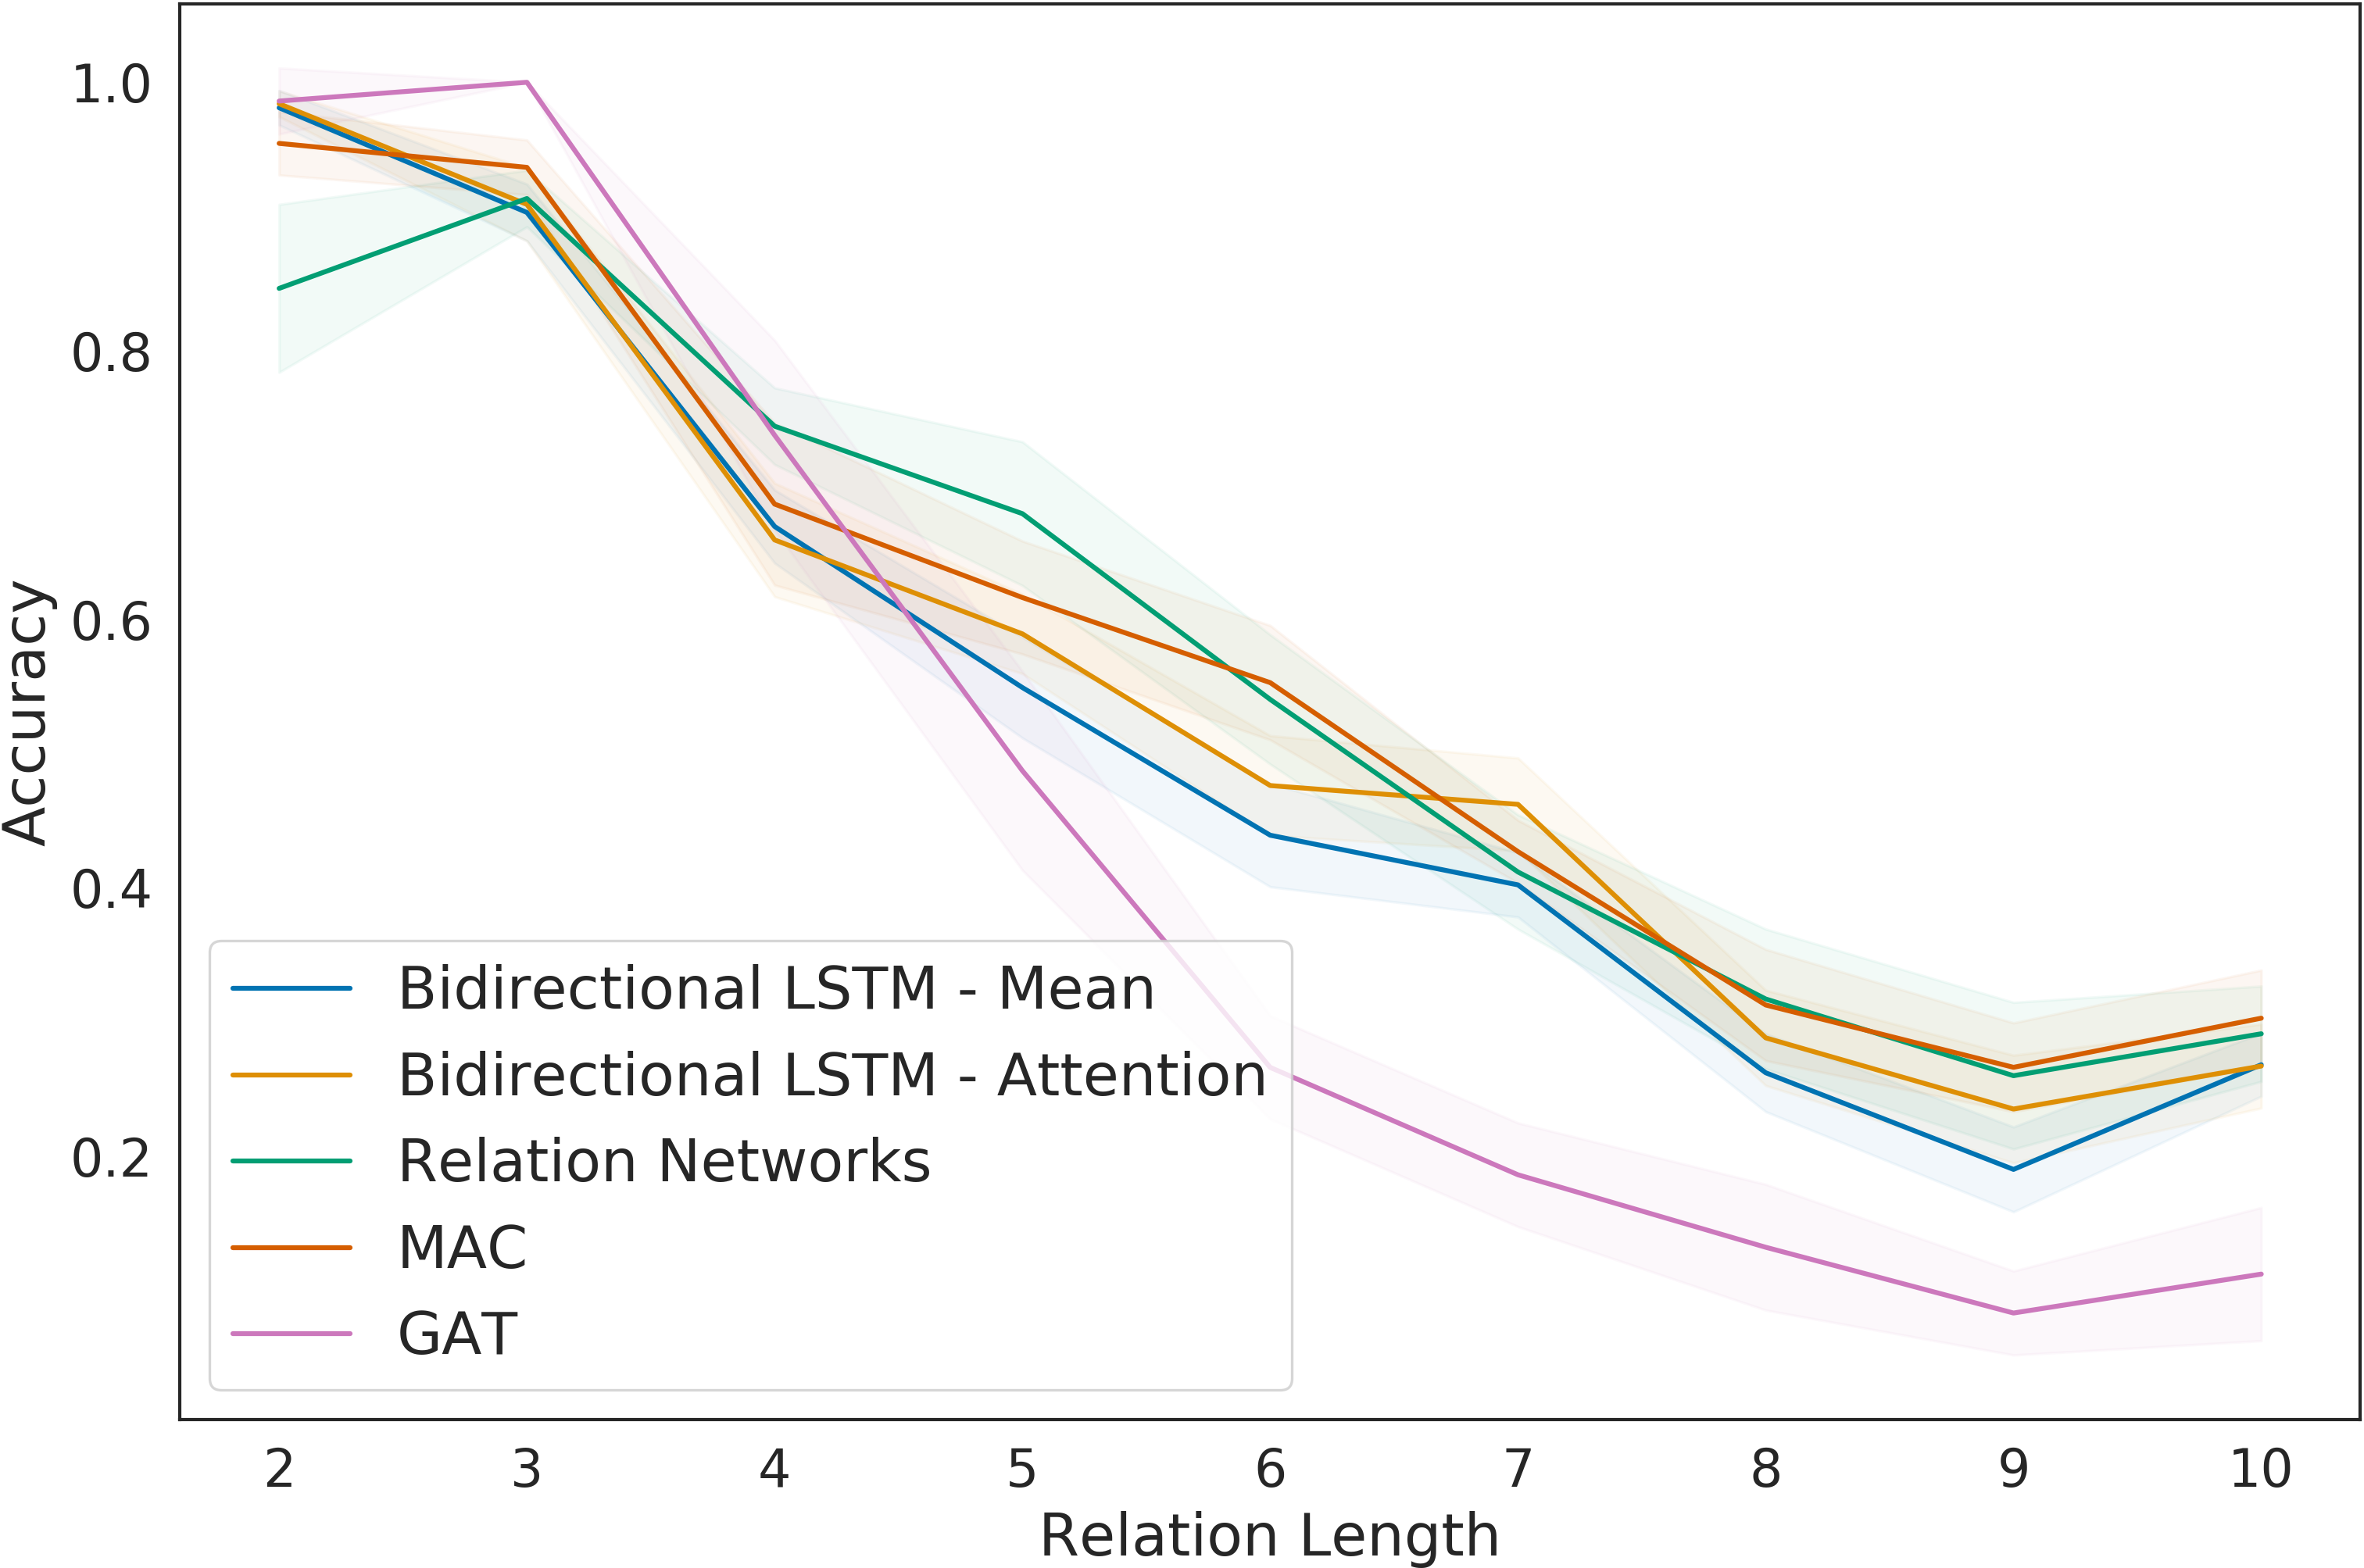
\includegraphics[width=0.48\textwidth]{figs/clutrr/sys_gen_amt_23.png} }}%
    \qquad
    \hspace{-20pt}
    \subfloat{{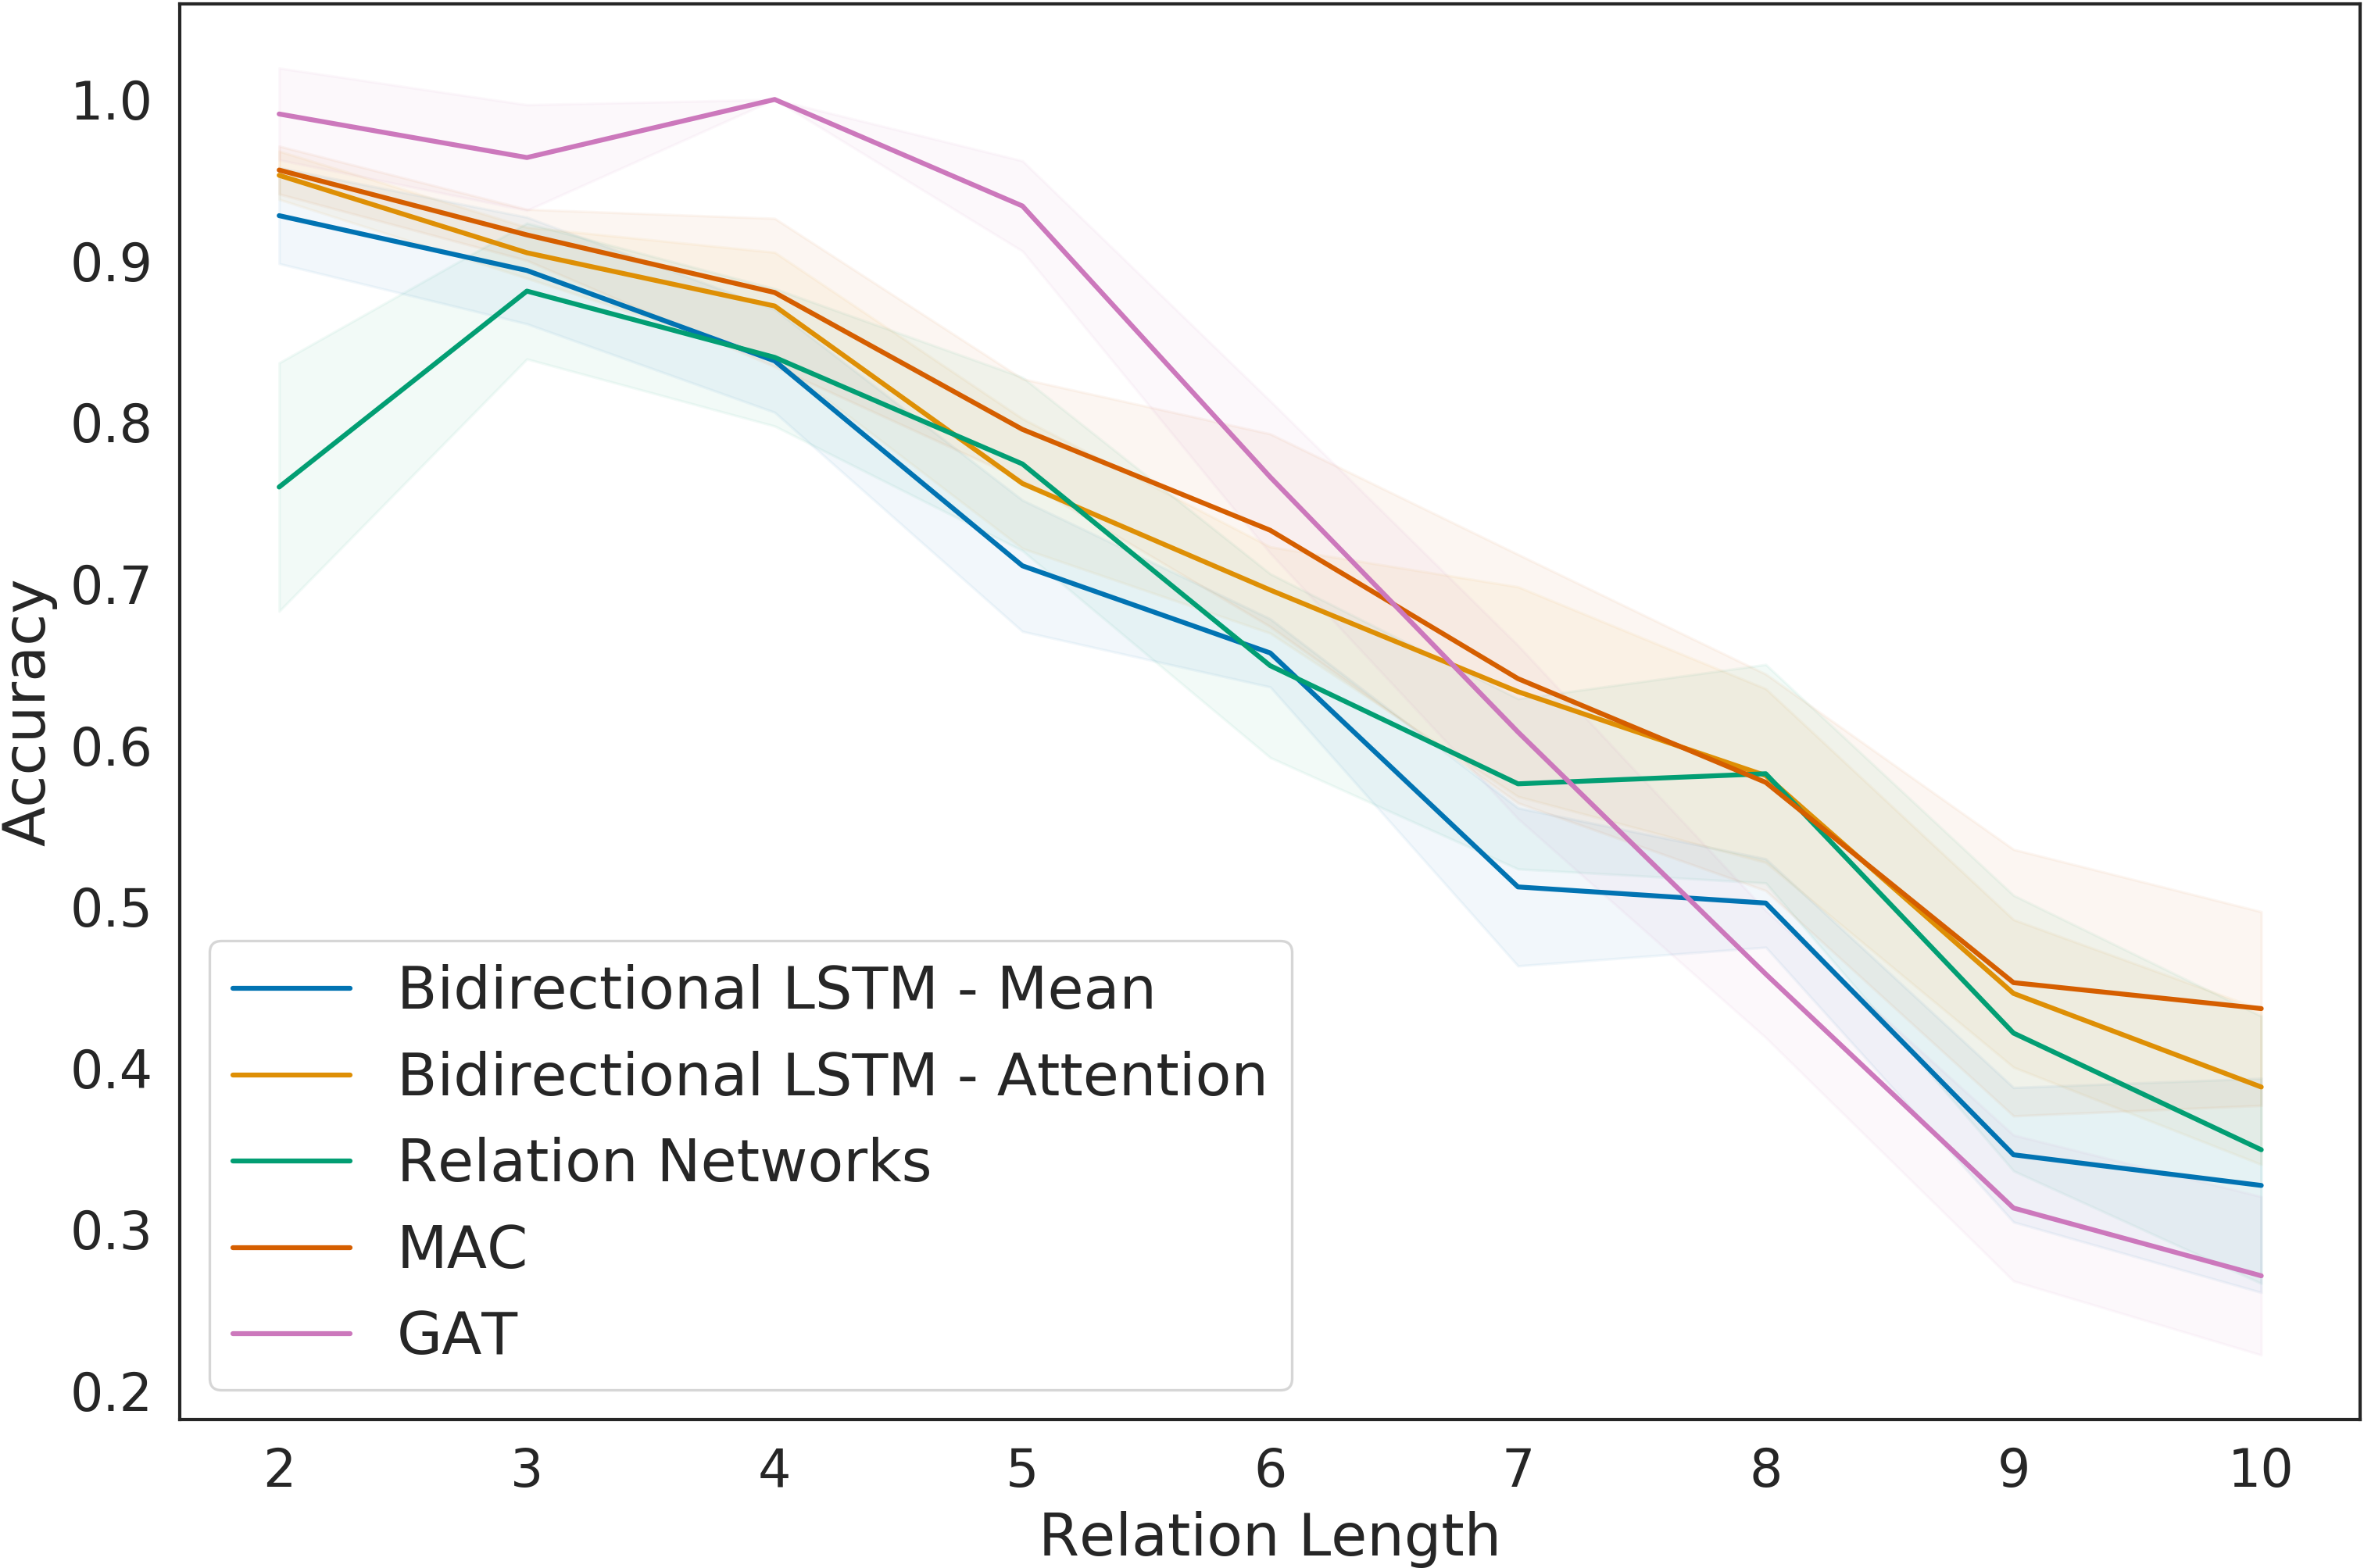
\includegraphics[width=0.48\textwidth]{figs/clutrr/sys_gen_amt_234.png} }}%
    \caption{Systematic Generalizability of different models on \texttt{CLUTRR-Gen} task (having 20\% less placeholders and without training and testing placeholder split), when {\bf Left:} trained with $k=2$ and $k=3$ and {\bf Right:} trained with $k=2,3$ and $4$}%
    \label{fig:gen_app_1}
\end{figure*}



To further confirm this trend, we ran experiments with modified train and test splits for the text-based models, where the same set of natural language paraphrases were used to construct the narratives in both the train and test splits (\autoref{fig:gen_app_1}). In this simplified setting, the text-based models must still learn to reason about held-out logical patterns, but the difficulty of parsing the natural language is essentially removed, as the same natural language paraphrases are used during testing and training. We found that the text-based models were competitive with the GAT model in this simplified setting, confirming that the poor performance of the text-based models on the main task is driven by the difficulty of parsing the unseen natural language narratives.

\subsection{Robust Reasoning}
\label{sec:clutrr_robust_reasoning}

\begin{table*}[t!]
\resizebox{\textwidth}{!}{
% Please add the following required packages to your document preamble:
% \usepackage{multirow}
\begin{tabular}{@{}cccccccc|c@{}}
\toprule
\multicolumn{1}{l}{} & \multicolumn{1}{l}{Models} & \multicolumn{6}{c}{Unstructured models (no graph)} & \multicolumn{1}{l}{Structured model (with graph)} \\ \midrule
\multicolumn{1}{l}{Training} & \multicolumn{1}{l|}{Testing} & BiLSTM - Attention & BiLSTM - Mean & RN & MAC & \multicolumn{1}{l}{BERT} & \multicolumn{1}{l|}{BERT-LSTM} & GAT \\ \midrule
Clean & \multicolumn{1}{c|}{Clean} & 0.58 \tiny $\pm 0.05$ & 0.53 \tiny $\pm 0.05$ & 0.49 \tiny $\pm 0.06$ & 0.63 \tiny $\pm 0.08$ & 0.37 \tiny $\pm 0.06$ & 0.67 \tiny $\pm 0.03$ & \textbf{1.0} \tiny $\pm 0.0$ \\ 
 & \multicolumn{1}{c|}{Supporting} & \textbf{0.76} \tiny $\pm 0.02$ & 0.64 \tiny $\pm 0.22$ & 0.58 \tiny $\pm 0.06$ & 0.71 \tiny $\pm 0.07$ & 0.28 \tiny $\pm 0.1$ & 0.66 \tiny $\pm 0.06$ & 0.24 \tiny $\pm 0.2$ \\
 & \multicolumn{1}{c|}{Irrelevant} & 0.7 \tiny $\pm 0.15$ & \textbf{0.76} \tiny $\pm 0.02$ & 0.59 \tiny $\pm 0.06$ & 0.69 \tiny $\pm 0.05$ & 0.24 \tiny $\pm 0.08$ & 0.55 \tiny $\pm 0.03$ & 0.51 \tiny $\pm 0.15$ \\
 & \multicolumn{1}{c|}{Disconnected} & 0.49 \tiny $\pm 0.05$ & 0.45 \tiny $\pm 0.05$ & 0.5 \tiny $\pm 0.06$ & 0.59 \tiny $\pm 0.05$ & 0.24 \tiny $\pm 0.08$ & 0.5 \tiny $\pm 0.06$ & \textbf{0.8} \tiny $\pm 0.17$ \\ \midrule
Supporting & \multicolumn{1}{c|}{Supporting} & 0.67 \tiny $\pm 0.06$ & 0.66 \tiny $\pm 0.07$ & 0.68 \tiny $\pm 0.05$ & 0.65 \tiny $\pm 0.04$ & 0.32 \tiny $\pm 0.09$ & 0.57 \tiny $\pm 0.04$ & \textbf{0.98} \tiny $\pm 0.01$ \\
\midrule
Irrelevant & \multicolumn{1}{c|}{Irrelevant} & 0.51 \tiny $\pm 0.06$ & 0.52 \tiny $\pm 0.06$ & 0.5 \tiny $\pm 0.04$ & 0.56 \tiny $\pm 0.04$ & 0.25 \tiny $\pm 0.06$ & 0.53 \tiny $\pm 0.06$ & \textbf{0.93} \tiny $\pm 0.01$ \\
\midrule
Disconnected & \multicolumn{1}{c|}{Disconnected} & 0.57 \tiny $\pm 0.07$ & 0.57 \tiny $\pm 0.06$ & 0.45 \tiny $\pm 0.11$ & 0.4 \tiny $\pm 0.1$ & 0.17 \tiny $\pm 0.05$ & 0.47 \tiny $\pm 0.06$ & \textbf{0.96} \tiny $\pm 0.01$ \\ \midrule
\multicolumn{1}{l}{Average} & \multicolumn{1}{c|}{} & \textbf{0.61} \tiny $\pm 0.08$ & 0.59 \tiny $\pm 0.08$ & 0.54 \tiny $\pm 0.07$ & \textbf{0.61} \tiny $\pm 0.06$ & 0.30 \tiny $\pm 0.07$ & 0.56 \tiny $\pm 0.05$ & \textbf{0.77} \tiny $\pm 0.09$ \\ \bottomrule
\end{tabular}}
\caption{Testing the robustness of the various models when training and testing on stories containing various types of noise facts. The types of noise facts (supporting, irrelevant, and disconnected) are defined in Section .}
\label{tab:robust}
\end{table*}


Finally, we use CLUTRR to systematically evaluate how various baseline neural language understanding systems cope with noise (\textbf{Q3}).
In all the experiments we provide a combination of $k=2$ and $k=3$ length clauses in training and testing, with noise facts being added to the train and/or test set depending on the setting (Table \ref{tab:robust}).
We use the different types of noise facts defined in Section \ref{sec:clutrr_robust_data}..

Overall, we find that the GAT baseline outperforms the unstructured text-based models across most testing scenarios (Table \ref{tab:robust}), which showcases the benefit of a structured feature space for robust reasoning.
When training on clean data and testing on noisy data, we observe two interesting trends that highlight the benefits and shortcomings of the various model classes:
\begin{enumerate}[leftmargin=*, topsep=2pt, itemsep=0pt]
    \item All the text-based models excluding BERT actually perform better when testing on examples that have {\em supporting} or {\em irrelevant} facts added. This suggests that these models actually benefit from having more content related to the entities in the story. Even though this content is not strictly useful or needed for the reasoning task, it may provide some linguistic cues (e.g., about entity genders) that the models exploit. In contrast, the BERT-based models do not benefit from the inclusion of this extra content, which is perhaps due to the fact that they are already built upon a strong language model (e.g., that already adequately captures entity genders.)
    \item  The GAT model performs poorly when {\em supporting} facts are added but has no performance drop when {\em disconnected} facts are added. This suggests that the GAT model is sensitive to changes that introduce cycles in the underlying graph structure but is robust to the addition of noise that is disconnected from the target entities.
\end{enumerate}

\subsubsection{Learning from noisy data}

Moreover, when we trained on noisy examples, we found that only the GAT model was able to consistently improve its performance (Table \ref{tab:robust}).
We notice that the GAT model, having access to the true underlying graph of the puzzles, perform better across different testing scenarios when trained with the noisy data. As the \textit{Supporting facts} contains cycles, it is difficult for GAT to generalize for a dataset with cycles when it is trained on a dataset without cycles. However, when trained with cycles, GAT learns to attend to \textit{all} the paths leading to the correct answer. This effect is disastrous when GAT is tested on \textit{Irrelevant facts} which contains dangling paths as GAT still tries to attend to all the paths. Training on \textit{Irrelevant facts} proved to be most beneficial to GAT, as the model now perfectly attends to \textit{only relevant paths}.
Since \textit{Disconnected facts} contains disconnected paths, the message passing function of the graph is unable to forward any information from the disjoint cliques, thereby having superior testing scores throughout several scenarios.

\begin{table*}[t!]
\resizebox{\textwidth}{!}{
% Please add the following required packages to your document preamble:
% \usepackage{multirow}
\begin{tabular}{@{}cccccccc|c@{}}
\toprule
\multicolumn{1}{l}{} & \multicolumn{1}{l}{Models} & \multicolumn{6}{c}{Unstructured models (no graph)} & \multicolumn{1}{l}{Structured model (with graph)} \\ \midrule
\multicolumn{1}{l|}{Training} & \multicolumn{1}{l|}{Testing} & BiLSTM - Attention & BiLSTM - Mean & RN & MAC & \multicolumn{1}{l}{BERT} & \multicolumn{1}{l|}{BERT-LSTM} & GAT \\ \midrule
Supporting & \multicolumn{1}{c|}{Clean} & 0.38 \tiny $\pm 0.04$ & 0.32 \tiny $\pm 0.04$ & 0.4 \tiny $\pm 0.09$ & 0.45 \tiny $\pm 0.03$ & 0.19 \tiny $\pm 0.06$ & 0.39 \tiny $\pm 0.06$ & \textbf{0.92} \tiny $\pm 0.17$ \\
\multicolumn{1}{l}{} & \multicolumn{1}{c|}{Supporting} & 0.67 \tiny $\pm 0.06$ & 0.66 \tiny $\pm 0.07$ & 0.68 \tiny $\pm 0.05$ & 0.65 \tiny $\pm 0.04$ & 0.32 \tiny $\pm 0.09$ & 0.57 \tiny $\pm 0.04$ & \textbf{0.98} \tiny $\pm 0.01$ \\
 & \multicolumn{1}{c|}{Irrelevant} & 0.44 \tiny $\pm 0.03$ & 0.39 \tiny $\pm 0.03$ & \textbf{0.51} \tiny $\pm 0.08$ & 0.46 \tiny $\pm 0.09$ & 0.2 \tiny $\pm 0.06$ & 0.36 \tiny $\pm 0.05$ & 0.5 \tiny $\pm 0.23$ \\
 & \multicolumn{1}{c|}{Disconnected} & 0.31 \tiny $\pm 0.21$ & 0.25 \tiny $\pm 0.16$ & 0.47 \tiny $\pm 0.08$ & 0.41 \tiny $\pm 0.06$ & 0.2 \tiny $\pm 0.08$ & 0.32 \tiny $\pm 0.04$ & \textbf{0.92} \tiny $\pm 0.05$ \\ \midrule
Irrelevant & \multicolumn{1}{c|}{Clean} & 0.57 \tiny $\pm 0.05$ & 0.56 \tiny $\pm 0.05$ & 0.46 \tiny $\pm 0.13$ & 0.67 \tiny $\pm 0.05$ & 0.24 \tiny $\pm 0.06$ & 0.46 \tiny $\pm 0.08$ & \textbf{0.92} \tiny $\pm 0.0$ \\
 & \multicolumn{1}{c|}{Supporting} & 0.38 \tiny $\pm 0.22$ & 0.31 \tiny $\pm 0.16$ & 0.61 \tiny $\pm 0.07$ & 0.61 \tiny $\pm 0.04$ & 0.27 \tiny $\pm 0.06$ & 0.46 \tiny $\pm 0.04$ & \textbf{0.77} \tiny $\pm 0.12$ \\
\multicolumn{1}{l}{} & \multicolumn{1}{c|}{Irrelevant} & 0.51 \tiny $\pm 0.06$ & 0.52 \tiny $\pm 0.06$ & 0.5 \tiny $\pm 0.04$ & 0.56 \tiny $\pm 0.04$ & 0.25 \tiny $\pm 0.06$ & 0.53 \tiny $\pm 0.06$ & \textbf{0.93} \tiny $\pm 0.01$ \\
 & \multicolumn{1}{c|}{Disconnected} & 0.44 \tiny $\pm 0.26$ & 0.54 \tiny $\pm 0.27$ & 0.55 \tiny $\pm 0.05$ & 0.61 \tiny $\pm 0.06$ & 0.26 \tiny $\pm 0.03$ & 0.45 \tiny $\pm 0.08$ & \textbf{0.85} \tiny $\pm 0.25$ \\ \midrule
\multirow{3}{*}{Disconnected} & \multicolumn{1}{c|}{Clean} & 0.45 \tiny $\pm 0.02$ & 0.47 \tiny $\pm 0.03$ & 0.53 \tiny $\pm 0.09$ & 0.5 \tiny $\pm 0.06$ & 0.22 \tiny $\pm 0.09$ & 0.44 \tiny $\pm 0.05$ & \textbf{0.75} \tiny $\pm 0.07$ \\
 & \multicolumn{1}{c|}{Supporting} & 0.47 \tiny $\pm 0.03$ & 0.46 \tiny $\pm 0.05$ & 0.54 \tiny $\pm 0.03$ & 0.58 \tiny $\pm 0.06$ & 0.22 \tiny $\pm 0.06$ & 0.38 \tiny $\pm 0.08$ & \textbf{0.78} \tiny $\pm 0.12$ \\
 & \multicolumn{1}{c|}{Irrelevant} & 0.47 \tiny $\pm 0.05$ & 0.48 \tiny $\pm 0.03$ & 0.52 \tiny $\pm 0.04$ & 0.51 \tiny $\pm 0.05$ & 0.17 \tiny $\pm 0.04$ & 0.38 \tiny $\pm 0.05$ & \textbf{0.56} \tiny $\pm 0.26$ \\
\multicolumn{1}{l}{} & \multicolumn{1}{c|}{Disconnected} & 0.57 \tiny $\pm 0.07$ & 0.57 \tiny $\pm 0.06$ & 0.45 \tiny $\pm 0.11$ & 0.4 \tiny $\pm 0.1$ & 0.17 \tiny $\pm 0.05$ & 0.47 \tiny $\pm 0.06$ & \textbf{0.96} \tiny $\pm 0.01$ \\ \midrule
\multicolumn{1}{l}{Average} & \multicolumn{1}{c|}{} & 0.47 \tiny $\pm 0.08$ & 0.46 \tiny $\pm 0.08$ & 0.52 \tiny $\pm 0.07$ & \textbf{0.53} \tiny $\pm 0.06$ & 0.23 \tiny $\pm 0.07$ & 0.43 \tiny $\pm 0.05$ & \textbf{0.82} \tiny $\pm 0.09$ \\ \bottomrule
\end{tabular}}
\caption{Testing the robustness of the various models when trained various types of noisy facts and evaluated on other noisy / clean facts.}
\label{tab:robust_appen}
\end{table*}


Again, these results highlights the performance gap between the unstructured text-based models and GAT for solving the CLUTRR task.

\subsubsection{Learning with synthetic placeholders}

In order to further understand the effect of language placeholders on robustness, we performed another set of experiments where we use bABI \cite{Weston2015-is} style simple placeholders (Table \ref{tab:robust_toy_appen}). We observe a marked increase in performance of all NLU models, where they significantly decrease the gap between their performance with that of GAT, even outperforming GAT on various settings. This shows the significance of using paraphrased placeholders in devising the complexity of the dataset.

\begin{table*}[t!]
\resizebox{\textwidth}{!}{
% Please add the following required packages to your document preamble:
% \usepackage{multirow}
\begin{tabular}{@{}cccccccc|c@{}}
\toprule
\multicolumn{1}{l}{} & \multicolumn{1}{l}{Models} & \multicolumn{6}{c}{Unstructured models (no graph)} & \multicolumn{1}{l}{Structured model (with graph)} \\ \midrule
\multicolumn{1}{l|}{Training} & \multicolumn{1}{l|}{Testing} & BiLSTM - Attention & BiLSTM - Mean & RN & MAC & \multicolumn{1}{l}{BERT} & \multicolumn{1}{l|}{BERT-LSTM} & GAT \\ \midrule
Supporting & \multicolumn{1}{c|}{Clean} & 0.96 \tiny $\pm 0.01$ & \textbf{0.97} \tiny $\pm 0.01$ & 0.88 \tiny $\pm 0.05$ & 0.94 \tiny $\pm 0.02$ & 0.48 \tiny $\pm 0.08$ & 0.57 \tiny $\pm 0.08$ & 0.92 \tiny $\pm 0.17$ \\
\multicolumn{1}{l}{} & \multicolumn{1}{c|}{Supporting} & 0.96 \tiny $\pm 0.03$ & 0.96 \tiny $\pm 0.03$ & 0.97 \tiny $\pm 0.01$ & 0.97 \tiny $\pm 0.01$ & 0.75 \tiny $\pm 0.07$ & 0.88 \tiny $\pm 0.05$ & \textbf{0.98} \tiny $\pm 0.01$ \\
 & \multicolumn{1}{c|}{Irrelevant} & 0.92 \tiny $\pm 0.02$ & \textbf{0.93} \tiny $\pm 0.01$ & 0.9 \tiny $\pm 0.03$ & 0.91 \tiny $\pm 0.01$ & 0.56 \tiny $\pm 0.04$ & 0.54 \tiny $\pm 0.06$ & 0.5 \tiny $\pm 0.23$ \\
 & \multicolumn{1}{c|}{Disconnected} & 0.8 \tiny $\pm 0.04$ & 0.83 \tiny $\pm 0.04$ & 0.76 \tiny $\pm 0.08$ & 0.86 \tiny $\pm 0.04$ & 0.27 \tiny $\pm 0.06$ & 0.42 \tiny $\pm 0.08$ & \textbf{0.92} \tiny $\pm 0.05$ \\ \midrule
Irrelevant & \multicolumn{1}{c|}{Clean} & 0.63 \tiny $\pm 0.02$ & 0.61 \tiny $\pm 0.07$ & 0.85 \tiny $\pm 0.09$ & 0.8 \tiny $\pm 0.07$ & 0.53 \tiny $\pm 0.09$ & 0.44 \tiny $\pm 0.06$ & \textbf{0.92} \tiny $\pm 0.0$ \\
 & \multicolumn{1}{c|}{Supporting} & 0.66 \tiny $\pm 0.03$ & 0.64 \tiny $\pm 0.04$ & 0.69 \tiny $\pm 0.06$ & 0.76 \tiny $\pm 0.06$ & 0.42 \tiny $\pm 0.08$ & 0.43 \tiny $\pm 0.08$ & \textbf{0.77} \tiny $\pm 0.12$ \\
\multicolumn{1}{l}{} & \multicolumn{1}{c|}{Irrelevant} & 0.89 \tiny $\pm 0.04$ & 0.86 \tiny $\pm 0.1$ & 0.74 \tiny $\pm 0.11$ & 0.78 \tiny $\pm 0.06$ & 0.61 \tiny $\pm 0.1$ & 0.83 \tiny $\pm 0.06$ & \textbf{0.93} \tiny $\pm 0.01$ \\
 & \multicolumn{1}{c|}{Disconnected} & 0.64 \tiny $\pm 0.02$ & 0.62 \tiny $\pm 0.05$ & 0.72 \tiny $\pm 0.05$ & 0.73 \tiny $\pm 0.04$ & 0.41 \tiny $\pm 0.04$ & 0.61 \tiny $\pm 0.05$ & \textbf{0.85} \tiny $\pm 0.25$ \\ \midrule
\multirow{3}{*}{Disconnected} & \multicolumn{1}{c|}{Clean} & 0.9 \tiny $\pm 0.05$ & 0.82 \tiny $\pm 0.12$ & \textbf{0.94} \tiny $\pm 0.02$ & 0.93 \tiny $\pm 0.04$ & 0.68 \tiny $\pm 0.07$ & 0.64 \tiny $\pm 0.02$ & 0.75 \tiny $\pm 0.07$ \\
 & \multicolumn{1}{c|}{Supporting} & 0.87 \tiny $\pm 0.04$ & 0.82 \tiny $\pm 0.05$ & 0.85 \tiny $\pm 0.03$ & \textbf{0.88} \tiny $\pm 0.04$ & 0.54 \tiny $\pm 0.08$ & 0.5 \tiny $\pm 0.05$ & 0.78 \tiny $\pm 0.12$ \\
 & \multicolumn{1}{c|}{Irrelevant} & \textbf{0.87} \tiny $\pm 0.03$ & 0.85 \tiny $\pm 0.03$ & 0.83 \tiny $\pm 0.03$ & 0.87 \tiny $\pm 0.02$ & 0.59 \tiny $\pm 0.09$ & 0.58 \tiny $\pm 0.09$ & 0.56 \tiny $\pm 0.26$ \\
\multicolumn{1}{l}{} & \multicolumn{1}{c|}{Disconnected} & 0.91 \tiny $\pm 0.04$ & 0.91 \tiny $\pm 0.03$ & 0.8 \tiny $\pm 0.17$ & 0.71 \tiny $\pm 0.11$ & 0.49 \tiny $\pm 0.1$ & 0.79 \tiny $\pm 0.1$ & \textbf{0.96} \tiny $\pm 0.01$ \\ \midrule
\multicolumn{1}{l}{Average} & \multicolumn{1}{c|}{} & 0.83 \tiny $\pm 0.08$ & 0.82 \tiny $\pm 0.08$ & 0.83 \tiny $\pm 0.07$ & \textbf{0.84} \tiny $\pm 0.06$ & 0.58 \tiny $\pm 0.07$ & 0.60 \tiny $\pm 0.05$ & \textbf{0.82} \tiny $\pm 0.09$ \\ \bottomrule
\end{tabular}}
\caption{Testing the robustness on toy placeholders of the various models when trained various types of noisy facts and evaluated on other noisy / clean facts.}
\label{tab:robust_toy_appen}
\end{table*}






% TODO insert figure
% \begin{center}
% 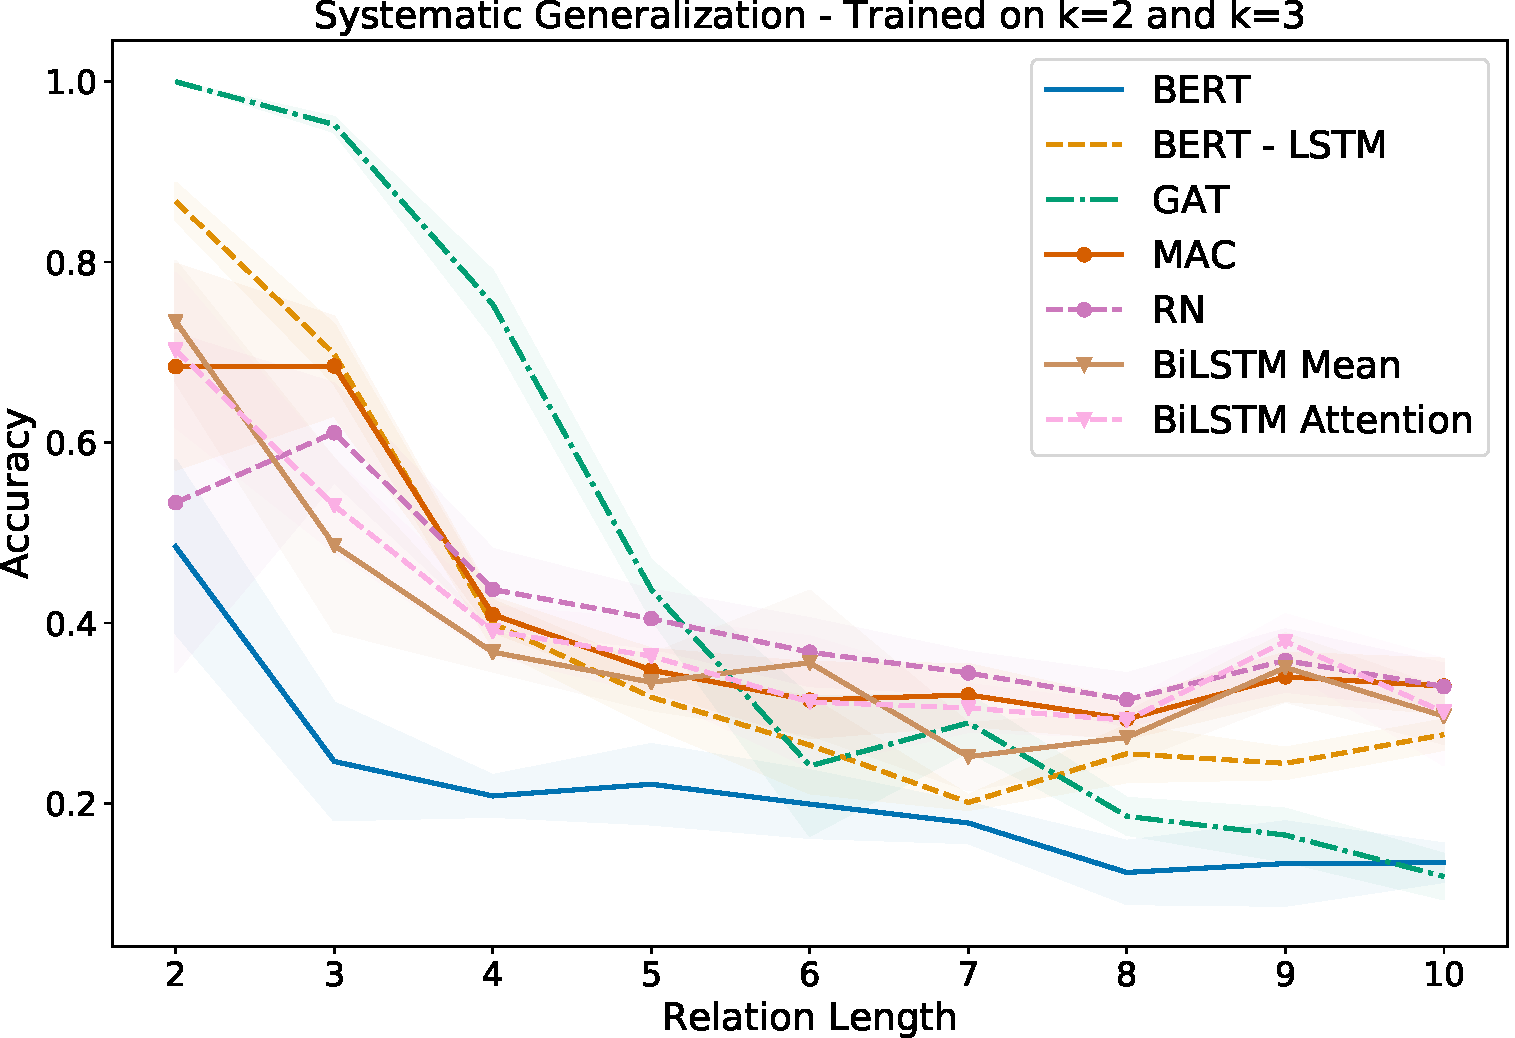
\includegraphics[height=0.3\textwidth]{figs/clutrr/emnlp/sys_gen_23.pdf}
% 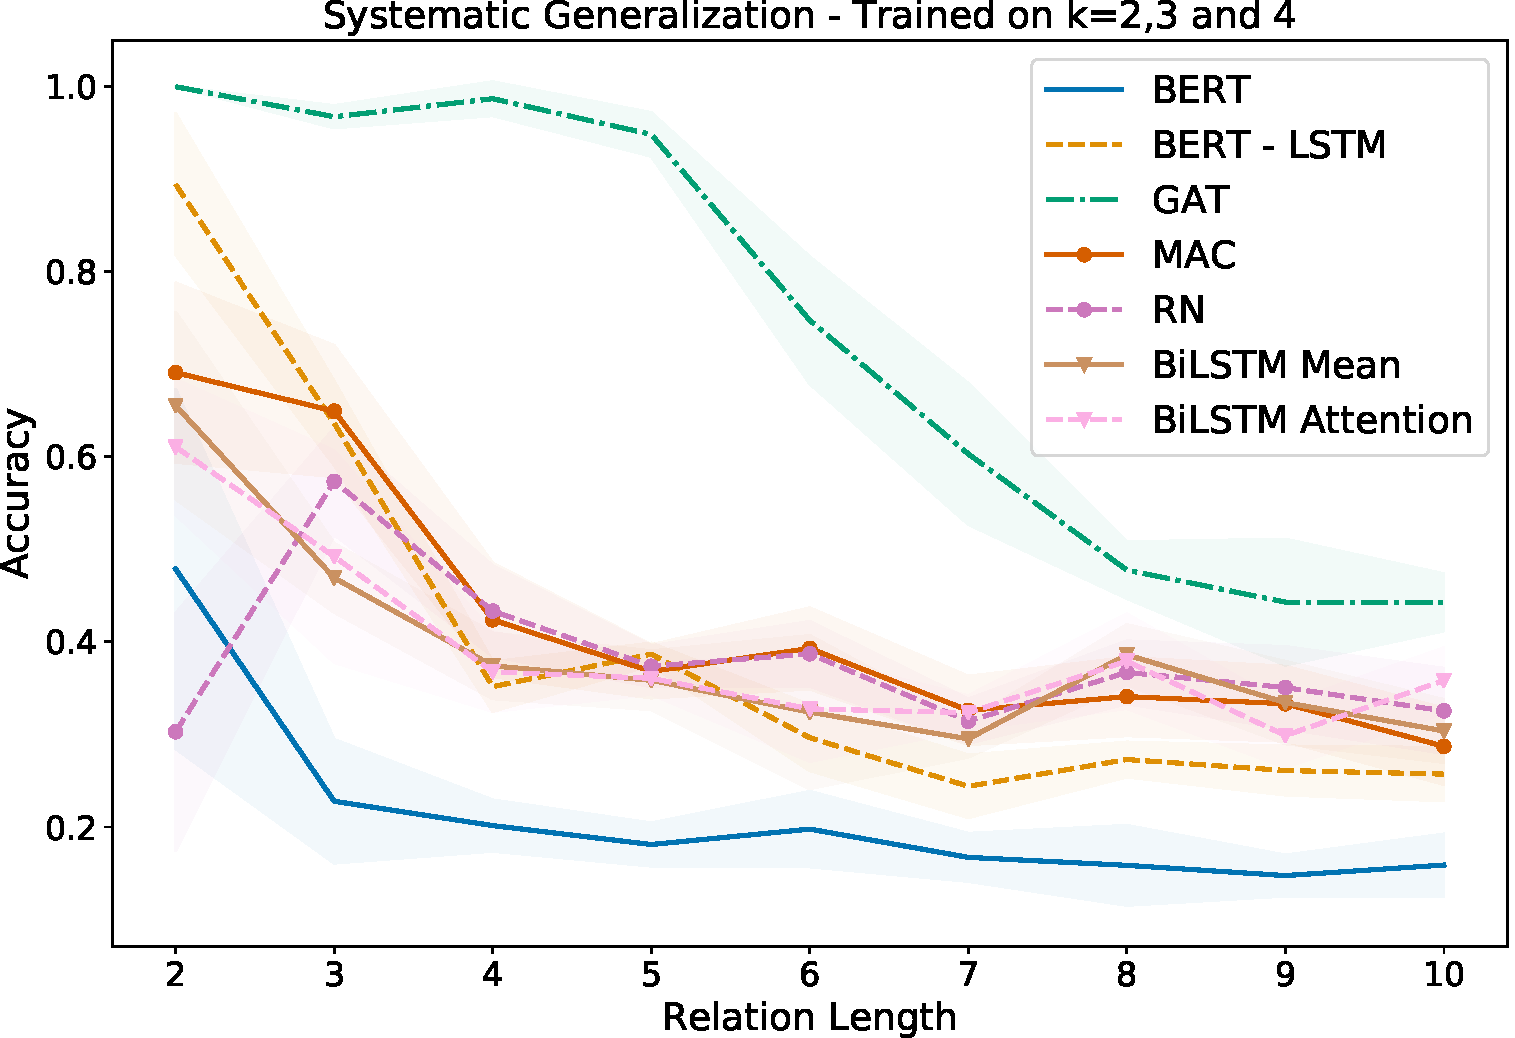
\includegraphics[height=0.3\textwidth]{figs/clutrr/emnlp/sys_gen_234.pdf}
% \end{center}
% \begin{figure}[htbp]
% \centering
% 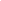
\includegraphics[height=0.0001in]{figs/empy_fig.png}
% \caption{Systematic generalization when train on k=\(2\) and \(3\).}
% \end{figure}


\section{Related Work}
\label{sec:clutrr_related_work}

To design the CLUTRR dataset, we draw inspiration from the classic work on inductive logic programming (ILP), a long line of reading comprehension benchmarks in NLP, as well as work combining language and knowledge graphs.

\subsection{Reading comprehension benchmarks}

Many datasets have been proposed to test the reading comprehension ability of NLP systems. This includes the SQuAD \cite{Rajpurkar2016-yc}, NewsQA \cite{Trischler2016-fc}, and MCTest \cite{richardson2013mctest} benchmarks that focus on factual questions; the SNLI \cite{bowman2015large} and MultiNLI \cite{williams2018broad} benchmarks for sentence understanding; and the bABI tasks \cite{Weston2015-is}, to name a few.
Our primary contribution to this line of work is the development of a carefully designed {\em diagnostic} benchmark to evaluate model robustness and systematic generalization in the context of NLU.

\subsection{Systematic generalization}

A growing body of literature has demonstrated that NLU models tend to exploit statistical artifacts in datasets and lack true generalization capabilities \cite{jia2017adversarial,gururangan2018annotation, kaushik2018much, lake2017generalization}.
These critical examinations have dovetailed with similar studies on visual question answering \citep{agrawal2016analyzing,bahdanau2018systematic,Johnson2016-mw}.
CLUTRR, contributes to this growing area by introducing a principled and flexible benchmark to evaluate systematic generalization in the context of language understanding---with our notion of systematic generalization being grounded in classic work on inductive logic programming (ILP) \cite{Quinlan1990-iv}.


\subsection{Question-answering with knowledge graphs}

Our work is also related to the domain of question answering and reasoning in knowledge graphs \citep{das2017go, xiong2018one, NIPS2018_7473, 8587330, xiong2017deeppath, welbl2018constructing, kartsaklis2018mapping}, where either the model is provided with a knowledge graph to perform inference over or where the model must infer a knowledge graph from the text itself.
However, unlike previous benchmarks in this domain---which are generally {\em transductive} and focus on leveraging and extracting knowledge graphs as a source of background knowledge about a fixed set of entities---CLUTRR requires {\em inductive logical reasoning}, where every example requires reasoning over a new set of previously unseen entities.


\section{Discussion}
\label{sec:clutrr_discussion}

In this paper we introduced the CLUTRR benchmark suite to test the systematic generalization and inductive reasoning capabilities of NLU systems.
We demonstrated the diagnostic capabilities of CLUTRR and found that existing NLU systems exhibit relatively poor robustness and systematic generalization capabilities---especially when compared to a graph neural network that works directly with symbolic input.
Concretely, using CLUTRR we were able to make the following key insights about the reasoning capability of modern neural networks:

\begin{itemize}
  \item \textbf{Neural language models are unable to reason when tested with systematicity.} We saw in \autoref{sec:clutrr_sys_gen} that the performance of all \acrshort{nlu} models drastically degrade when we test on instances which require systematicity - the knowledge of combination of existing parts - to solve the task. While all models had access to all possible rules (by ingesting a combination of relations in the training data), all models are notably worse when tested with longer chain of reasoning than the ones trained upon. This shortcoming could be due to overly associating to certain patterns seen during training, or learning to solve the task by taking shortcuts - associating some combination of tokens for certain relations \citep{gururangan2018annotation}.
  \item \textbf{Models are not robust in their language understanding.} When evaluated with enabling (supporting) and distractor information (noise), we observe models to display conflicting results. While supporting information is indeed useful for certain classes of models (\autoref{sec:clutrr_robust_reasoning}), irrelevant and distracting information also seems to aide in the reasoning process, which is not a systematic behaviour. Furthermore, when trained with noise, majority of the \acrshort{nlu} models are unable to discern between the correct and the incorrect information. These results indicate a potential surface form realization issue.
  \item \textbf{The key hurdle behind systematic generalization is the natural language itself.} Finally, we observe overwhelmingly that when a model which is only provided a graph, stripped of the natural language layer, the model is able to reason with surprising ability. The graph model, GAT, does not have to extract the relevant information from a given free-form text. This makes it easier for the model to generalize more effectively, even in the scenarios when the model is tasked to learn from distractor (noisy) information.
\end{itemize}

These results highlight the gap that remains between machine reasoning models that work with unstructured text and models that are given access to more structured input. It appears the key hindrance for a neural model for effective generalization and reasoning is the access to proper surface forms. These results raises questions on the syntax processing capabilities of \acrshort{nlu} models, and call for more in-depth investigation on the same. In fact, in the following chapters of this thesis, I will discuss my works on further studying the notions of syntax encoding in \acrshort{nlu} models using the tool of systematicity.

\section{Follow-up findings in the community}
\label{sec:clutrr_followup}


\clearpage
\chapter{Quantifying syntactic generalization using word order}
\label{sec:unli}

Of late, large scale pre-trained Transformer-based \citep{vaswani-etal-2017-attention} models---such as RoBERTa \citep{liu-et-al-2019-roberta}, BART \citep{lewis-etal-2020-bart}, and GPT-2 and -3 \citep{radford-etal-2019-language,brown-etal-2020-gpt3}---have exceeded recurrent neural networks' performance on many NLU tasks \citep{wang-etal-2018-glue, wang-etal-2019-superglue}. %The success of these models has prompted serious investigation, leading some to claim that pre-trained transformers can capture a surprising amount of lexical and semantic knowledge \cite{}, on the basis of their performance on either large benchmark suites \citep{wang-etal-2018-glue, wang-etal-2019-superglue} or on specialized test sets designed to evaluate linguistic knowledge \citep{linzen-etal-2016-assessing,  mccoy-etal-2019-right}.
Several papers have even suggested that Transformers pretrained on a language modeling (LM) objective can capture syntactic information \citep{hewitt-manning-2019-structural,jawahar-etal-2019-bert, warstadt-bowman-2020-can, wu-etal-2020-perturbed}, with their self-attention layers being capable of surprisingly effective learning \cite{rogers2020}.
In the preceeding chapter, we observed that \acrshort{nlu} models, including BERT, are unable to reason systematicity, primarily due to their lack of understanding the surface forms of the given task. Thus, in this chapter, we question the claim that state-of-the-art \acrshort{nlu} models ``know syntax''.

Since there are many ways to investigate ``syntax'', we must be clear on what we mean by the term.
Knowing the syntax of a sentence means being sensitive to the \textit{order of the words} in that sentence (among other things).  Humans are sensitive to word order, so clearly, ``language is not merely a bag of words'' \citep[p.156]{harris-1954-distributional}.
Moreover, it is easier for us to identify or recall words presented in canonical orders than in disordered, ungrammatical sentences; this phenomenon is called the \textit{``sentence superiority effect''} (\citealt{cattell-1886-time, scheerer1981early, toyota-2001-changes, baddeley-etal-2009-working, snell-grainger-2017-sentence, snell2019word, wen-etal-2019-parallel}, i.a.).
This effect also finds some neurobiological support from work showing ordered text activates portions of the temporal lobe more than unordered word lists \citep{bemis-pylkkanen-2013-basic, pylkkanen-etal-2014-building}.
In our estimation then, if one wants to claim that  a model ``knows syntax'', then they should minimally show that the model is sensitive to word order (at least for e.g. English or Mandarin Chinese).

Generally, knowing the syntax of a sentence is taken to be a prerequisite for understanding what that sentence means \citep{heim-kratzer-1998-semantics}.
Models should have to know the syntax first then, if performing any particular NLU task that genuinely requires a humanlike understanding of meaning (cf. \citealt{bender-koller-2020-climbing}).
Thus, if our models are as good at NLU as our current evaluation methods suggest, we should expect them to be sensitive to word order.
In this chapter, I discuss our paper \cite{sinha-etal-2021-unnatural} where we use a suite of permutation metrics to find the models are not sensitive to word order.
% We find, based on a suite of permutation metrics, that they are not.

\begin{table}[t]
    \centering
    \small
    \begin{adjustbox}{max width=0.95\linewidth}
    \begin{tabular}{p{11em}p{9em}p{3em}} % I hate the vertical line, can we get rid of it...
    \toprule
     \bf Premise & \bf Hypothesis & \bf Predicted Label \\ \midrule
    Boats in daily use lie within feet of the fashionable bars and restaurants.  & There are boats close to bars and restaurants. & E \\
    \addlinespace[0.5em]
    restaurants and use feet of fashionable lie the in Boats within bars daily . & bars restaurants are There and to close boats . & E \\ \midrule
    He and his associates weren't operating at the level of metaphor. & He and his associates were operating at the level of the metaphor. & C\\  \addlinespace[0.5em]
    his at and metaphor the of were He operating associates n't level . & his the and metaphor level the were He at associates operating of . & C\\
    \bottomrule
    \end{tabular}
   \end{adjustbox}
    \caption{Examples from the MNLI Matched development set. Both the original example and the permuted one elicit the same classification label (entailment and contradiction respectively) from RoBERTa (large).
    A simple demo is provided in an associated \href{https://colab.research.google.com/drive/1vv8Xmag1go3dib4vZXUZXAFB4ltDaMH7?usp=sharing}{Google Colab notebook.}}
    \label{tab:unli:example}
\end{table}



%Given the ``sentence superiority effect", if NLI models are reasoning through sentences in a humanlike way, they should be unsure of how to classify an ungrammatical, syntax corrupted premise-hypothesis pair .
 % for which no word is present in its original position , and the relative word ordering is minimized .
We focus here on textual entailment, one of the hallmark tasks used to measure how well models understand language \citep{condoravdi-etal-2003-entailment, dagan-etal-2005-pascal}. This task, often also called Natural Language Inference (NLI; \citealt{bowman-etal-2015-large}, i.a.), typically consists of two sentences: a premise and a hypothesis. The objective is to predict whether the premise entails the hypothesis, contradicts it, or is neutral with respect to it.  We find rampant word order insensitivity in purportedly high performing NLI models. %, somewhat surprisingly,
For nearly all premise-hypothesis pairs, \textbf{there are many permuted examples that fool the models} into providing the correct prediction. In case of MNLI, for example, the current state-of-the-art of 90.5\% can be increased to \textbf{98.7}\% merely by permuting the word order of test set examples. We even find drastically increased cross-dataset generalization when we reorder words. This is not just a matter of chance---we show that the model output probabilities are significantly different from uniform. A sample of the model outputs with permuted examples is shown in \autoref{tab:unli:example}.

We verify our findings with three popular English NLI datasets---SNLI \citep{bowman-etal-2015-large}, MultiNLI \citep{williams-etal-2018-broad} and ANLI \citep{nie-etal-2020-adversarial})---%By performing such iterative sampling, we can find a permuted subset of popular NLI datasets which achieves near perfect performance.
and one Chinese one, OCNLI \cite{hu-etal-2020-ocnli}. It is thus less likely that our findings result from some quirk of English or a particular tokenization strategy.
We also observe the effect for various transformer architectures pre-trained on language modeling (RoBERTa \citep{liu-et-al-2019-roberta}, BART \citep{lewis-etal-2020-bart}, DistilBERT \citep{sanh2020distilbert}), and non-transformers, including a ConvNet  \citep{zhao2015self}, an InferSent model \citep{conneau-etal-2017-supervised}, and a BiLSTM \citep{collobert2008unified}.
% We further expand our investigation to capture a probabilistic statistics on the acceptance of permutations for each example. We investigate the root cause of the effect, and find high model confidence of over-parameterized models to be one such factor. We also find n-gram overlap of permuted sentences is correlated with model performance on permuted sentences, while the sentences with the least n-gram overlap also reflects high acceptability. We devise a novel Part-of-Speech Minitree hypothesis to further explain the scenario of randomized sentence acceptability, and find our hypothesis correlates with model performance as well. Finally, we devise a simple alternative training regime based on maximizing the entropy of the model on randomized sentences, and find it being effective at reducing the acceptability probability of the language understanding models considerably, without hurting the original model performance.

Thus, in this chapter I discuss our contributions in \citet{sinha-etal-2021-unnatural}, which are as follows:
(i) we propose a suite of metrics (\textit{\PermAcc}) for measuring model insensitivity to word order (\autoref{sec:unli_exp_setup}),
(ii) we construct multiple permuted test datasets for measuring NLI model performance at a large scale (\autoref{sec:unli_results}),
% Since we are moving this section to appendix, should we mention it here?
(iii) we show that NLI models focus on words more than word order, but can partially reconstruct syntactic information from words alone (\autoref{sec:unli_pos_mini_tree}), %, as we explore with metrics for word overlap and Part-of-Speech overlap, and
(iv) we show the problem persists on out-of-domain data,
(v) we show that humans struggle with UnNatural Language Inference, underscoring the non-humanlikeness of SOTA models (\autoref{sec:unli_human_eval}),
(vi) finally, we explore a simple maximum entropy-based method (\autoref{sec:unli_training}) to encourage models not to accept permuted examples.





\section{Technical Background}
\label{sec:unli_technical_bg}

In this chapter, we investigate the task of Natural Language Inference (NLI), also known as Recognizing Textual Entailment (RTE). NLI task consists of inferring the logical relation between two sentences, typically known as the \textit{premise} and the \textit{hypothesis}. The logical relations that can exist between these two sentences can be on of three types: \textit{entailment} if the premise \textit{entails} the hypothesis, \textit{contradiction} if it is the opposite, and \textit{neutral} if the sentences have non overlapping meaning. Historically, this logical relation formulation is derived from \textit{natural logic} \citep{maccartney-manning-2007-natural}, which consisted of seven set-theoretic relations between any given pair of sentences. We use the formulation prescribed by \cite{bowman-etal-2015-large}, which is the simplified formulation consisting of the three standard relations.

Linguists generally take syntactic structure to be necessary for humans to know what sentences mean. Many also find the NLI task to a very promising approximation of human natural language understanding, in part because it is rooted in the tradition of logical entailment. In the spirit of propositional logic, sentence meaning is taken to be %the spirit of many propositional logics with
truth-conditional \citep{frege1948sense, montague-1970-universal, chierchia-mcconnell-1990-meaning, heim-kratzer-1998-semantics}. That is to say that understanding a sentence is equivalent to knowing the actual conditions of the world under which the sentences would be (judged) true \citep{wittgenstein-1922-tractatus}. If grammatical sentences are required for sentential inference, as per a truth conditional approach \citep{montague-1970-universal}, then permuted sentences should be meaningless. Put another way, the meanings of highly permuted sentences (if they exist) are not propositions, and thus those sentences don't have truth conditions. Only from their truth conditions of sentences can we tell if a sentence entails another.
In short, the textual entailment task is technically undefined in our ``unnatural'' setting. %Given our working definitions of textual entailment from the NLI task, it's not reasonable to say, for example, whether ``The the yesterday bit dog hard man'' is entailed by ``The man bit the dog hard yesterday'' or not.


Since existing definitions don't immediately extend to unnatural word orders, we outline several hypothetical \textit{systematic} ways that a model might perform, had it been sensitive to word order. We hypothesize two models that operate on the first principles of NLI, and one that doesn't. In the first case, Model A deems permuted sentences meaningless (devoid of truth values), as formal semantic theories of human language would predict. Thus, it assigns \textit{``neutral"} to every permuted example. Next, Model B does not deem permuted sentences meaningless, and attempts to understand them. Humans find understanding permuted sentences difficult (see our human evaluations in \autoref{sec:unli_human_eval}). Model B could also similarly struggle to decipher the meaning, and just equally sample labels for each example (i.e., assigns equal probability mass to the outcome of each label). Finally, we hypothesize a non-systematic model, Model C, which attempts to treat permuted sentences as though they weren't permuted at all. This model could operate similarly as bag-of-words (BOW), and thus always assign the same label to the permuted examples as it would to the un-permuted examples. If the model failed to assign the original gold label to the original unpermuted examples, it will also fail to assign the original gold label to its permutations; it will never get higher accuracy on permuted examples than on unpermuted ones.

We find in our experiments that the state-of-the-art Transformer-based NLI models (as well as pre-Transformer class of models) do not perform like any of the above hypothetical models. They perform closest to Model C, but are, in some cases, actually able to achieve \emph{higher} accuracy on permuted examples. To better quantitatively describe this behaviour,
we introduce our suite of \textbf{\PermAcc} metrics that enable us to quantify how accepting models are of permuted sentences.


\section{Experimental Setup}
\label{sec:unli_exp_setup}

\subsection{Constructing the permuted dataset.}

For a given dataset $D$ having splits $D_{\text{train}}$ and $D_{\text{test}}$, we first train an NLI model $M$ on $D_{\text{train}}$ to achieve comparable accuracy to what was reported in the original papers. We then construct a randomized version of $D_{\text{test}}$, which we term as $\hat{D}_{\text{test}}$ such that: for each example $(p_i,h_i,y_i) \in D_{\text{test}}$ (where $p_i$ and $h_i$ are the premise and hypothesis sentences of the example respectively and $y_i$ is the gold label), we use a permutation operator $\mathcal{F}$ that returns a list ($\hat{P}_i, \hat{H}_i$) of $q$ permuted sentences ($\hat{p}_i$ and $\hat{h}_i$), where $q$ is a hyperparameter. $\mathcal{F}$ essentially permutes all positions of the words in a given sentence (i.e., either in premise or hypothesis) with the restriction that \textit{no words maintain their original position}.  In our initial setting, we do not explicitly control the placement of the words relative to their original neighbors, but we analyze clumping effects in \autoref{sec:unli_results}.
$\hat{D}_{\text{test}}$ now consists of $|D_{\text{test}}| \times q$ examples, with $q$ different permutations of hypothesis and premise for each original test example pair. If a sentence $S$ (e.g., $h_i$) contains $w$ words, then the total number of available permutations of $S$ are $(w-1)!$, thus making the output of $\mathcal{F}$ a list of $(w-1)! \choose q$ permutations in this case. For us, the space of possible outputs is larger, since we permute $p_i$ and $h_i$ separately (and ignore examples for which any $|S|\leq5$).

\subsection{Defining \PermAcc.}

The choice of $q$ naturally allows us to analyze a statistical view of the predictability of a model on the permuted sentences. To that end, we define the following notational conventions. Let $\mathcal{A}$ be the original accuracy of a given model $M$ on a dataset $D$, and \textit{c} be the number of examples in a dataset which are marked as correct according to the standard formulation of accuracy for the original dataset (i.e., they are assigned the ground truth label). Typically $\mathcal{A}$ is given by $\frac{c}{|D_{test}|}$ or $\frac{c}{|D_{dev}|}$. %, where $c$ is the number of examples assigned the ground truth label.

\begin{figure}[t]
    \centering
    \resizebox{0.5\textwidth}{!}{
        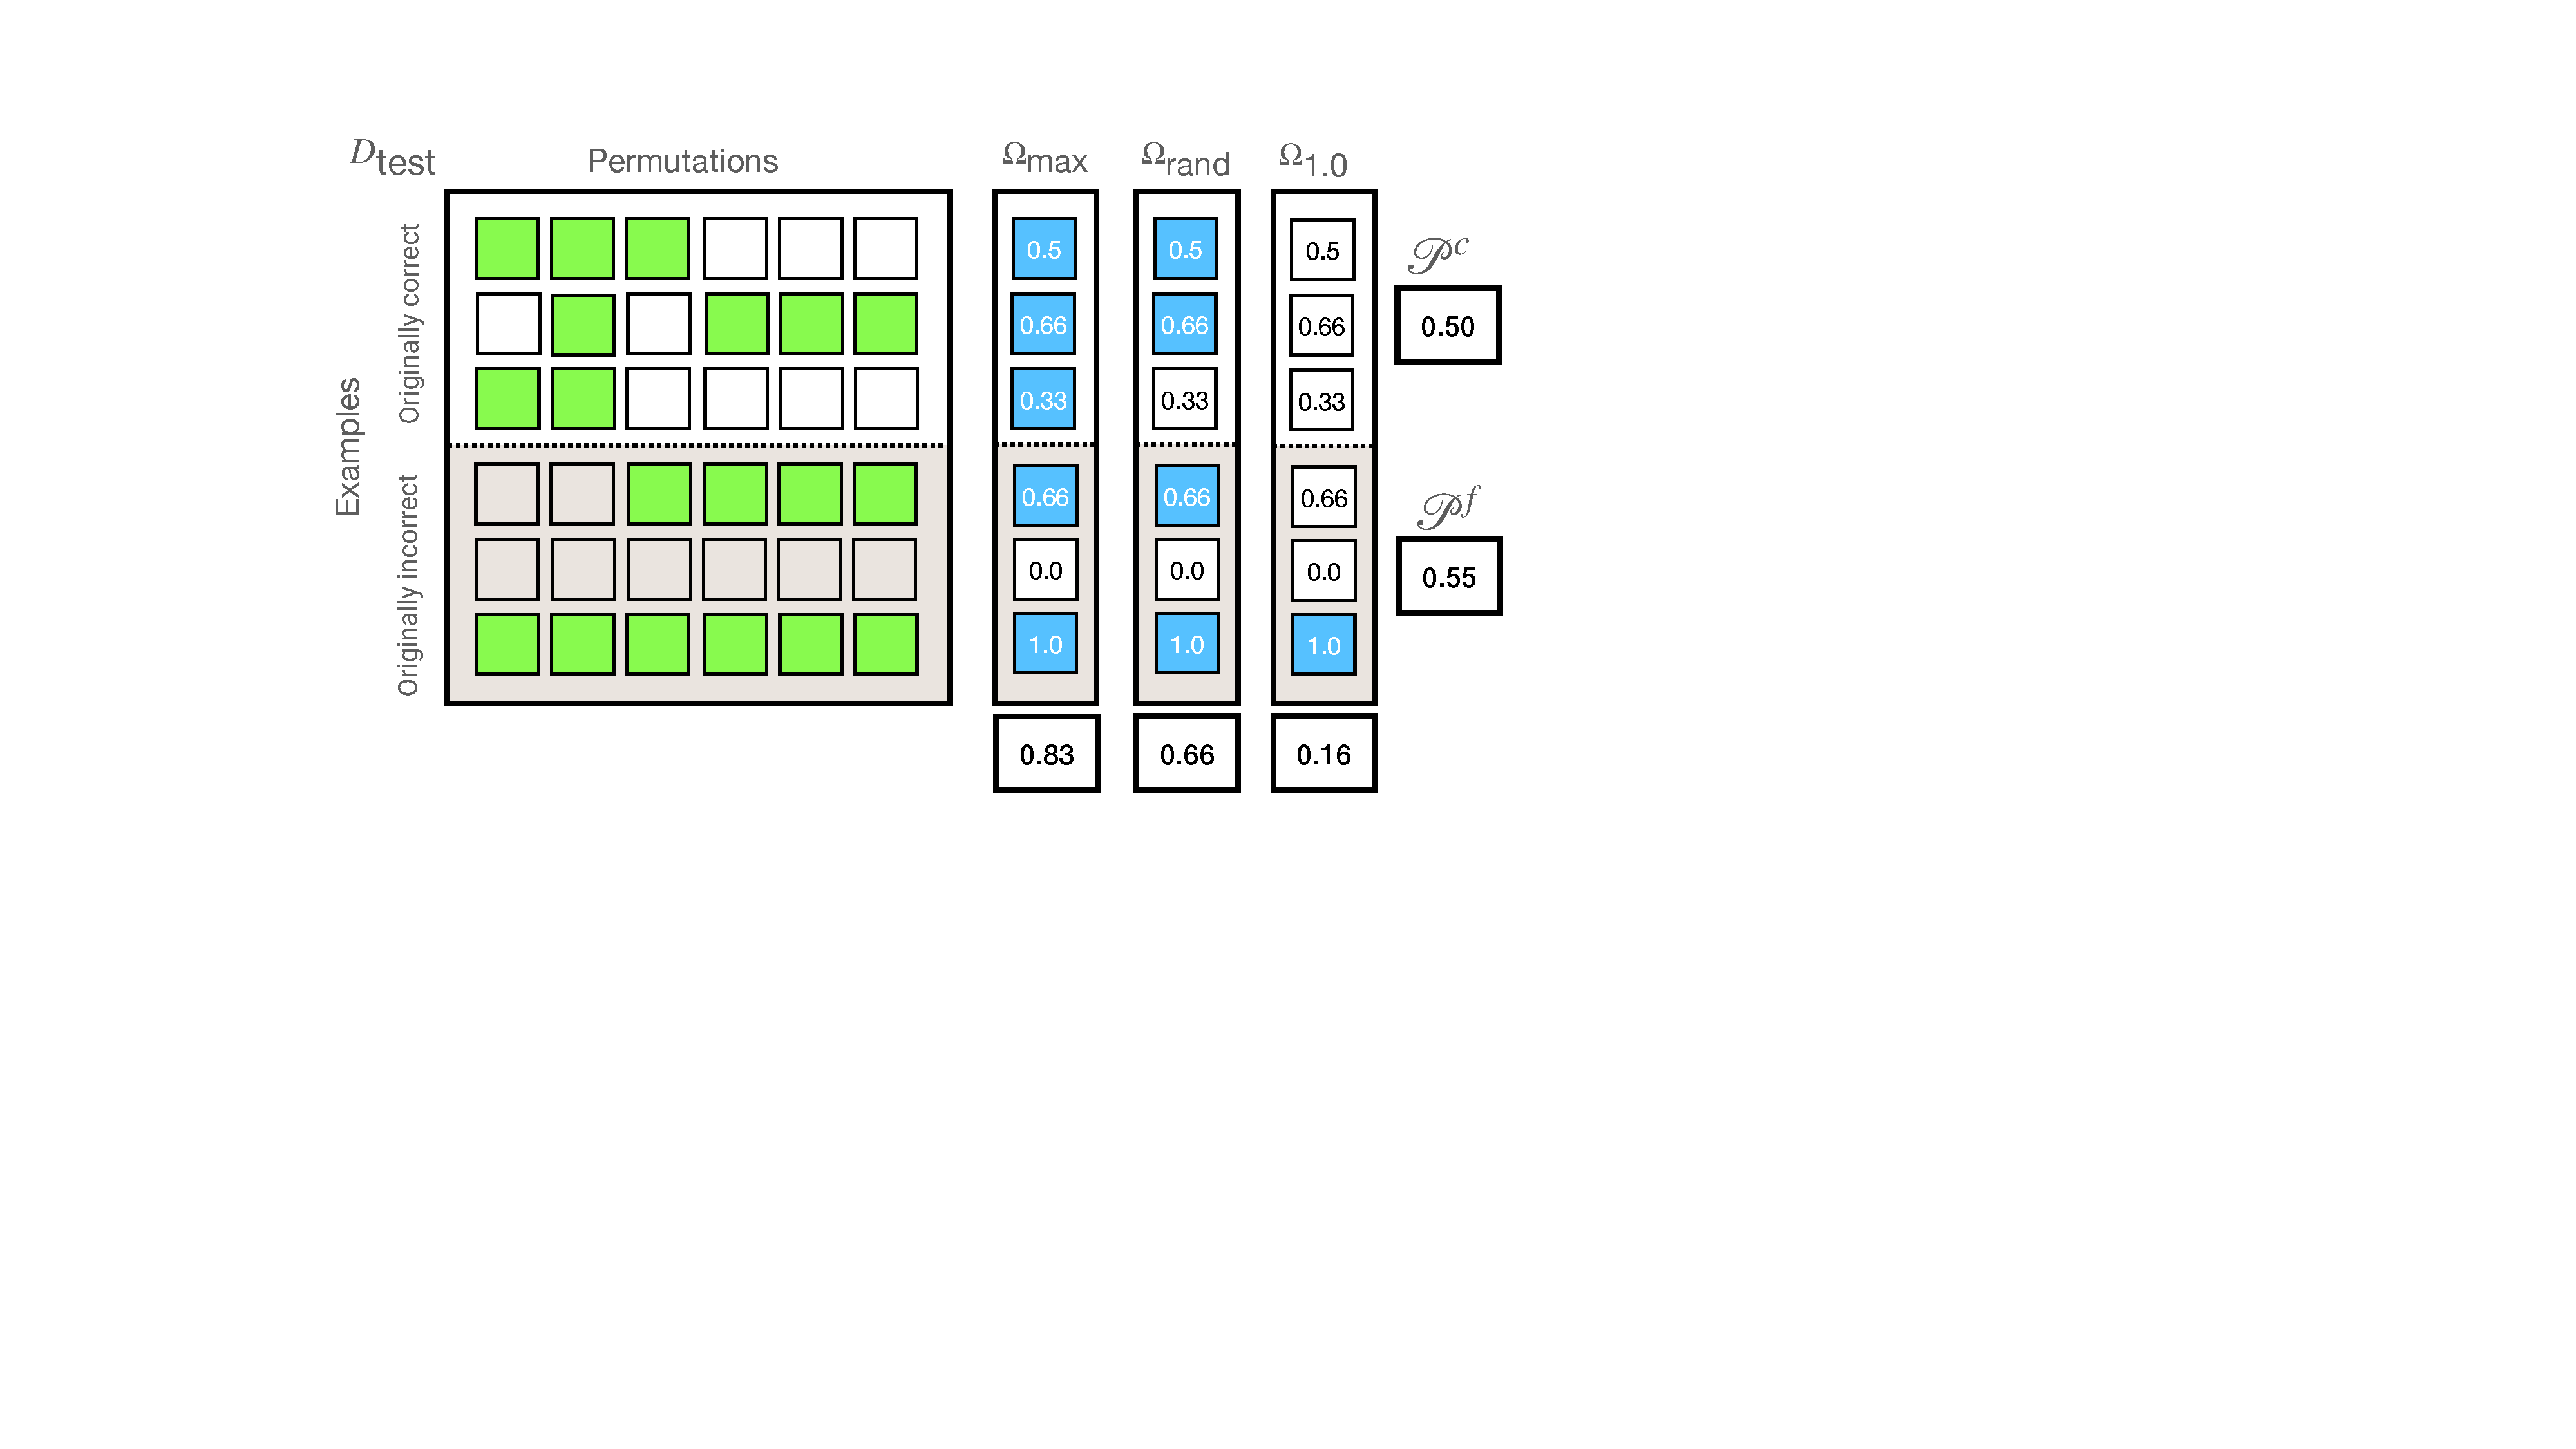
\includegraphics{figs/unli/nli_gen_perm_desc.pdf}}
    \caption{Graphical representation of the \PermAcc\ class of metrics. Given a sample test set ${D}_{\text{test}}$ with six examples, three of which originally predicted correctly (model predicts gold label), three incorrectly (model fails to predict gold label), with $n=6$ permutations, $\Omega_{\text{max}}$,$\Omega_{\text{rand}}$, $\Omega_{\text{1.0}}$, $\mathcal{P}^c$ and $\mathcal{P}^f$ are provided. Green boxes indicate permutations accepted by the model. Blue boxes mark examples that crossed each threshold and were used to compute the corresponding metric. }
    \label{fig:def_metrics}
\end{figure}

Let $\Pr_{M}(\hat{P}_i, \hat{H}_i)_{\text{cor}}$ then be the percentage of $q$ permutations of an example $(p_i, h_i)$ assigned the ground truth label $y_i$ by $M$:
   % \begin{equation}
    %\begin{split}
    \begin{align}
    &&\Pr_{M}(\hat{P}_i, \hat{H}_i)_{\text{cor}} =
    \frac{1}{q}\sum_{\mathclap{(\hat{p}_j \in \hat{P}_i, \hat{h}_j \in \hat{H}_i)}}((M(\hat{p}_j, \hat{h}_j) = y_i) \rightarrow 1)
    \end{align}
    %\end{split}
    %\end{equation}
To get an overall summary score, we let $\Omega_x$ be the percentage of examples $(p_i, h_i) \in D_{\text{test}}$ for which $\Pr_{M}(\hat{P}_i, \hat{H}_i)_{\text{cor}}$ exceeds a predetermined threshold $0 < x < 1$. %Concretely, $\Omega_x$ is defined as the percentage of examples in $D_{\text{test}}$, for which the probability of model accepting the permutation as the correct answer is greater than $x$ percent.
Concretely, a given example will count as correct according to $\Omega_x$ if more than $x$ percent of its permutations ($\hat{P}_i$ and $\hat{H}_i$) are assigned $y_i$ by the model $M$.
Mathematically,
    \begin{align} %I don't love this, but it fits...\mathrlap right centers the subscript, if it's centered it overlaps the D_test
    %\begin{split}
    &&\Omega_x = \frac{1}{\mid D_{test}\mid} \sum_{\mathrlap{(p_i, h_i)\in D_{test}}} ((\Pr_{M}(\hat{P}_i, \hat{H}_i)_{\text{cor}}
    > x) \rightarrow 1).
    %\end{split}
    \end{align}
There are two specific cases of $\Omega_{\text{x}}$ that we are most interested in. First, we define $\Omega_{\text{max}}$ or the \textbf{Maximum Accuracy}, where $x = 1 / |D_{\text{test}}|$. In short, $\Omega_{\text{max}}$ gives the percentage of examples $(p_i, h_i) \in D_{\text{test}}$ for which there is \textit{at least one} permutation $(\hat{p_j}, \hat{h_j})$ that model $M$ assigns the gold label $y_i$
% new: added comment on omega_max tending towards 1
\footnote{Theoretically, $\Omega_{\text{max}} \rightarrow 1$ if the number of permutations $q$ is large. Thus, in our experiments we set $q=100$.}.
Second, we define $\Omega_{\text{rand}}$, or \textbf{Random Baseline Accuracy}, where $x = 1 / m$ or chance probability (for balanced $m$-way classification, where $m=3$ in NLI). This metric is less stringent than $\Omega_{\text{max}}$, as it counts an example if at least \textit{one third} of its permutations are assigned the gold label (hence provides a lower-bound relaxation). See \autoref{fig:def_metrics} for a graphical representation of $\Omega_{\text{x}}$.

We also define %\textit{Flip}
$D^{f}$ to be the list of examples originally marked incorrect according to $\mathcal{A}$, but are now deemed correct according $\Omega_{\text{max}}$. $D^{c}$ is the list of examples originally marked correct according to  $\mathcal{A}$. Thus, we should expect $D^{f}<D^{c}$ for models that have high accuracy.
Additionally, we define $\mathcal{P}^c$ and $\mathcal{P}^f$, as the dataset average percentage of permutations which predicted the gold label, when the examples were originally correct ($D^{c}$) and when the examples were originally incorrect ($D^{f}$) as per $\mathcal{A}$ (hence, flipped) respectively.
\begin{equation}
\begin{split}
    &\mathcal{P}^{c} = \frac{1}{|D^{c}|} \sum_{i=0}^{|D^{c}|} M(\hat{P}_i, \hat{H}_i)_{\text{cor}}\\
    % &\mathcal{P}^f = \frac{1}{|D^{f}|} \sum_{i=0}^{|D^f|} M(\hat{P}_i, \hat{H}_i)_{\text{cor}}
\end{split}
\end{equation}

\noindent $P^f$ is defined similarly by replacing $D^c$ by $D^f$. Note that for a classic BOW model,  $\mathcal{P}^c=100$ and $\mathcal{P}^f=0$, because it would rely on the words alone (not their order) to make its classification decision. Since permuting removes no words, BOW models should come to the same decisions for permuted examples as for the originals.



\section{Evaluated Models}


We run our experiments on two types of models: \textbf{(a)} Transformer-based models and \textbf{(b)} Non-Transformer Models. In \textbf{(a)}, we investigate the state-of-the-art pre-trained models such as RoBERTa-Large \cite{liu-et-al-2019-roberta}, BART-Large \cite{lewis-etal-2020-bart} and DistilBERT \cite{sanh2020distilbert}. For \textbf{(b)} we consider several recurrent and convolution based neural networks, such as InferSent \cite{conneau-etal-2017-supervised}, Bidirectional LSTM \cite{collobert2008unified} and ConvNet \cite{zhao2015self}. We train all models on MNLI, and evaluate on in-distribution (SNLI and MNLI) and out-of-distribution datasets (ANLI). We independently verify results of \textbf{(a)} using both our fine-tuned model using HuggingFace Transformers \cite{wolf2020transformers} and pre-trained checkpoints from FairSeq \cite{ott2019fairseq} (using PyTorch Model Hub). For \textbf{(b)}, we use the InferSent codebase. We sample $q=100$ permutations for each example in $D_{\text{test}}$, and use 100 seeds for each of those permutations to ensure full reproducibility. We drop examples from test sets where we are unable to compute \textit{all unique} randomizations, typically these are examples with sentences of length of less than 6 tokens. \footnote{Code, data, and model checkpoints are available at \href{https://github.com/facebookresearch/unlu}{https://github.com/facebookresearch/unlu}.}



\section{Results}
\label{sec:unli_results}

\subsection{Models accept many permuted examples.}
\label{sec:unli_results_accept}

\begin{figure}[ht]
    \centering
    \resizebox{0.7\linewidth}{!}{
        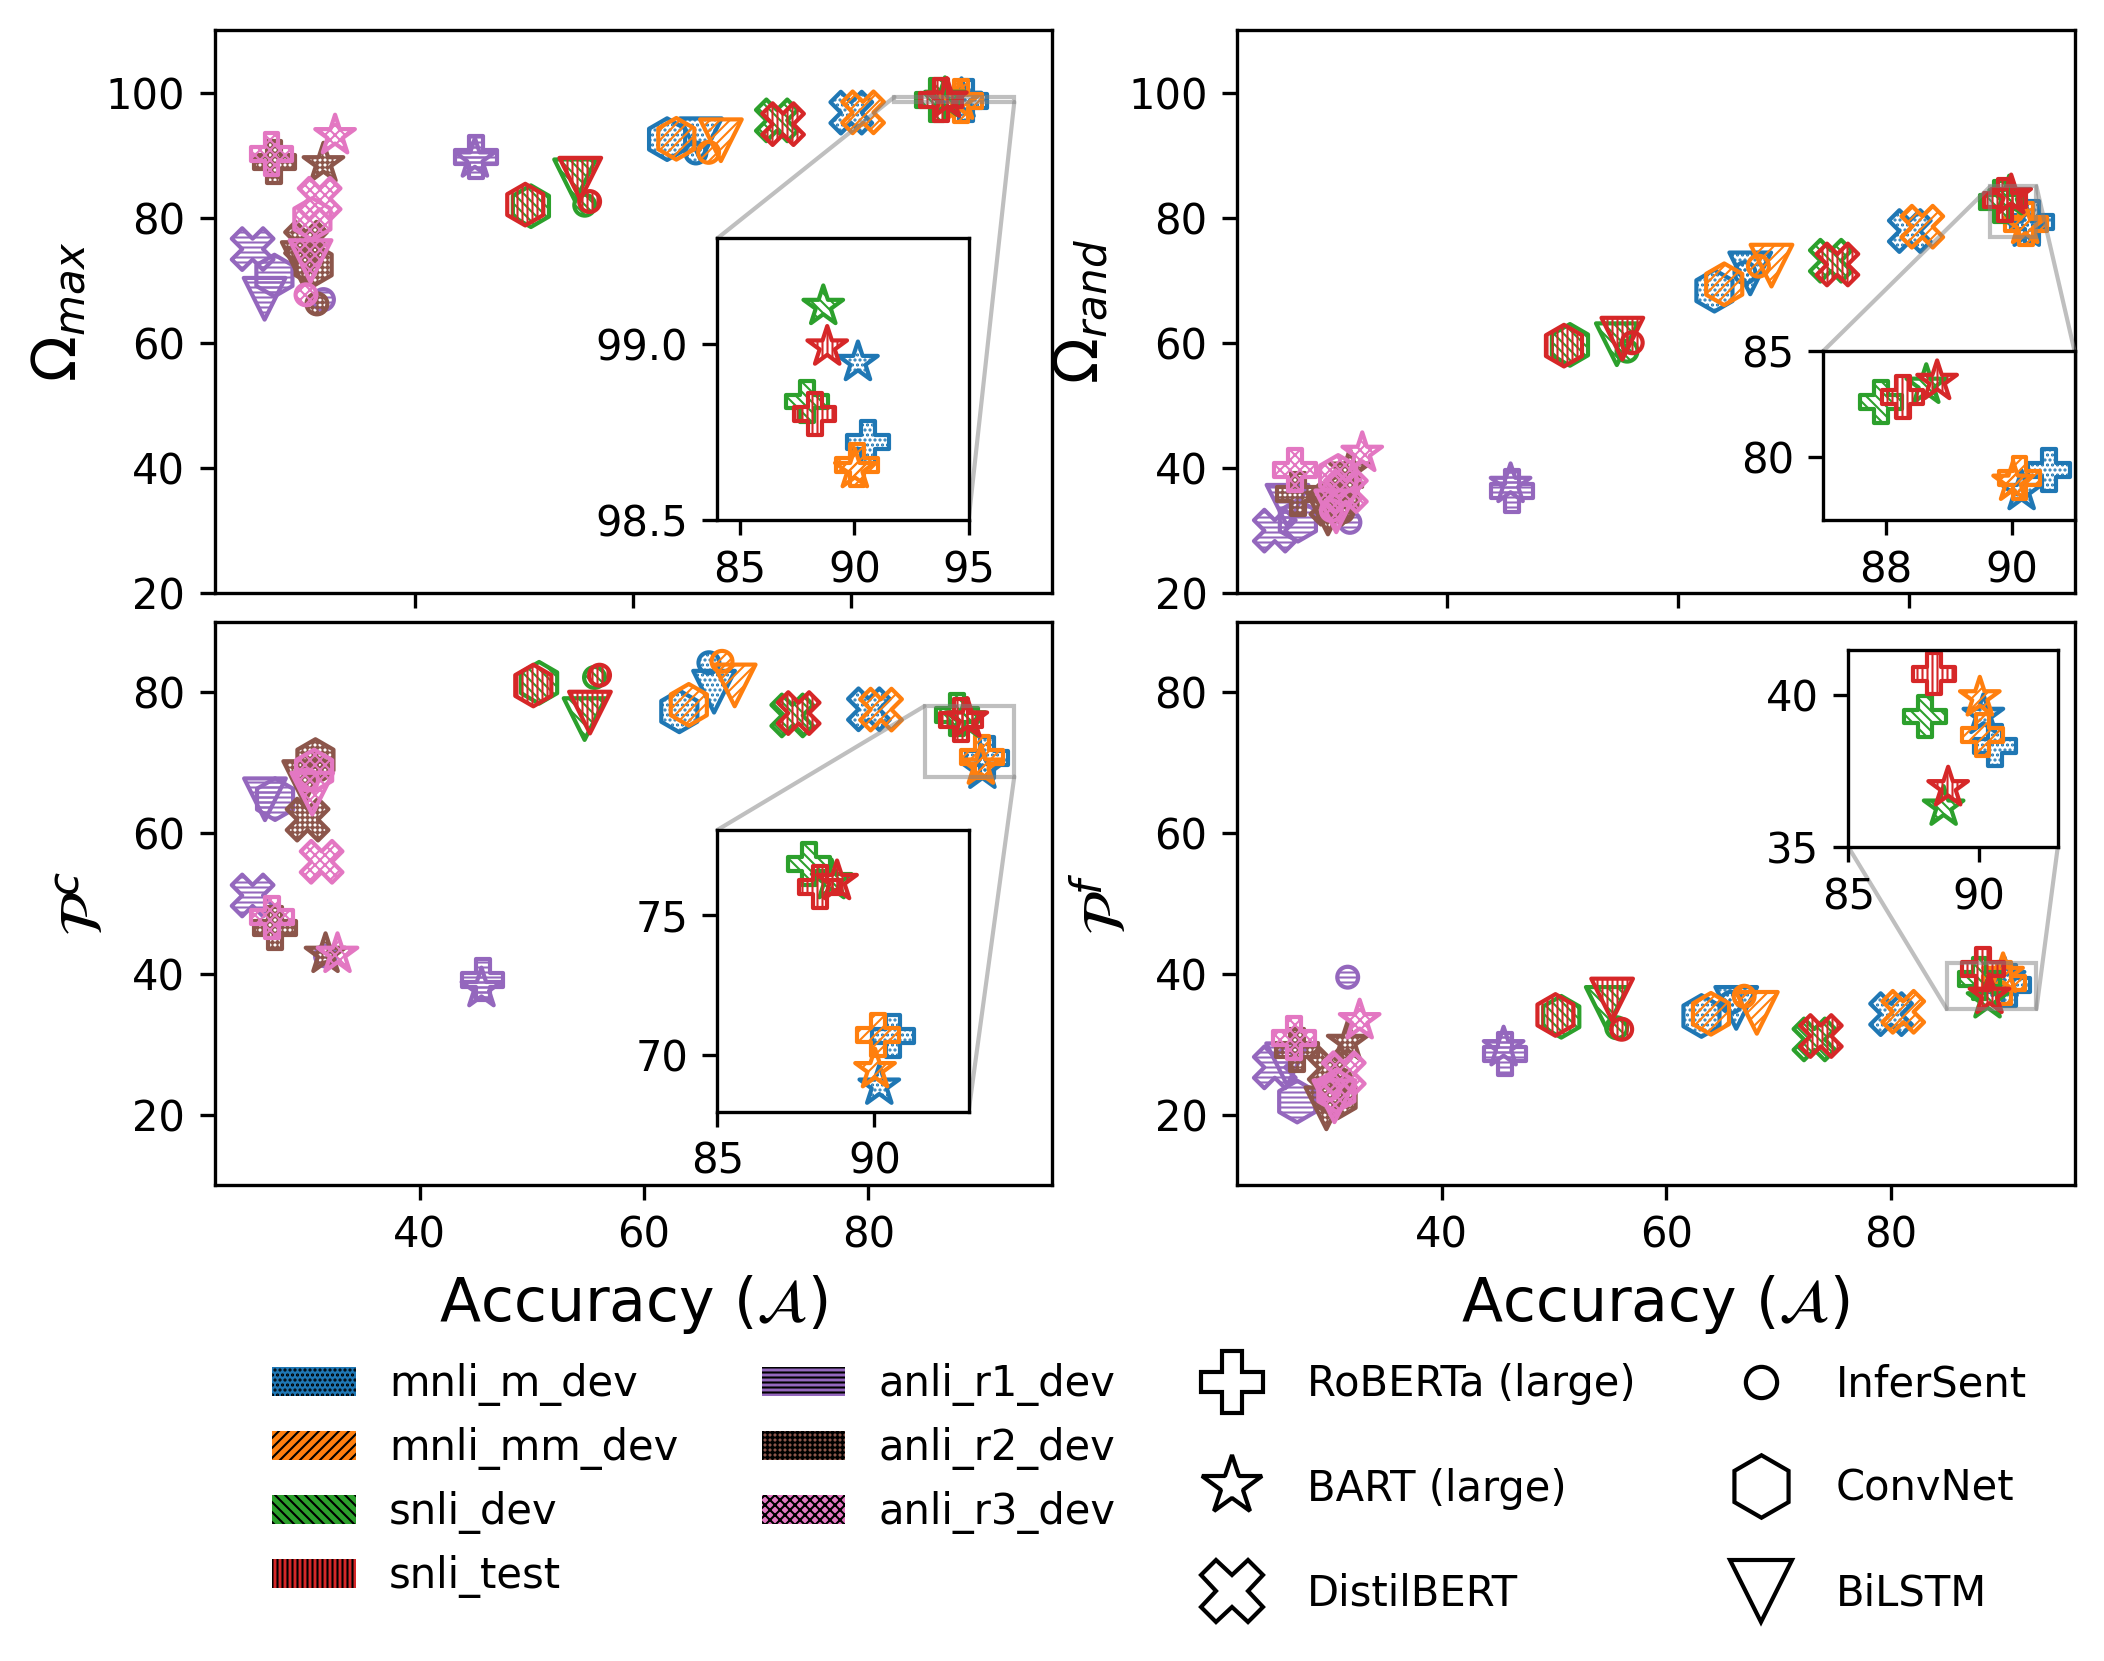
\includegraphics{figs/unli/comb_plot_0.png}}
    \caption{Comparison of $\Omega_{\text{max}}$,$\Omega_{\text{rand}}$,$\mathcal{P}^c$ and $\mathcal{P}^f$ with the model accuracy $\mathcal{A}$ on multiple datasets, where all models are trained on the MNLI corpus \cite{williams-etal-2018-broad}.}
    \label{fig:comb_plot}
\end{figure}

We find $\Omega_{\text{max}}$ is very high for models trained and evaluated on MNLI (in-domain generalization), reaching \textbf{98.7\%} on MNLI dev. and test sets (in RoBERTa, compared to $\mathcal{A}$ of 90.6\% (\autoref{table:unli_main}). Recall, human accuracy is approximately 92\% on MNLI dev.,  \citealt{nangia-bowman-2019-human}). This shows that there exists at least one permutation (usually many more) for almost all examples in $D_{\text{test}}$ such that model $M$ predicts the gold label. We also observe high $\Omega_{\text{rand}}$ at 79.4\%, showing that there are many examples for which the models outperform even a random baseline in accepting permuted sentences. We provide an example of the behaviour in \autoref{tab:unli:example}.

Evaluating out-of-domain generalization with ANLI dataset splits resulted in an $\Omega_{\text{max}}$ value that is notably higher than $\mathcal{A}$ (89.7\% $\Omega_{\text{max}}$ for RoBERTa compared to 45.6\% $\mathcal{A}$). As a consequence, we encounter many \textit{flips}, i.e., examples where the model is unable to predict the gold label, but at least one permutation of that example is able to. However, recall this analysis expects us to know the gold label upfront, so this test can be thought of as running a word-order probe test on the model until the model predicts the gold label (or give up by exhausting our set of $q$ permutations). For out-of-domain generalization, $\Omega_{\text{rand}}$ decreases considerably (36.4\% $\Omega_{\text{rand}}$ on A1), which means fewer permutations are accepted by the model. Next, recall that a classic bag-of-words model would have $\mathcal{P}^c=100$ and $\mathcal{P}^f=0$. No model performs strictly like a classic bag of words although they do perform somewhat BOW-like ($\mathcal{P}^c >> \mathcal{P}^f$ for all test splits, \autoref{fig:comb_plot}). %Although it is harder to find the correct permutation for already misclassified, non-generalizable sentences, state-of-the-art models still behave somewhat BOW-like.
We find this BOW-likeness to be higher for certain non-Transformer models, (InferSent) as they exhibit higher $\mathcal{P}^c$ (84.2\% for InferSent compared to 70.7\% for RoBERTa on MNLI).


\begin{table}[htbp]
  \centering
  \resizebox{0.5\linewidth}{!}{%
    \begin{tabular}{@{}llrrrrr@{}}
\toprule
           Model &    Eval. Dataset  &  $\mathcal{A}$ &  $\Omega_{\text{max}}$ &  $\mathcal{P}^c$ &  $\mathcal{P}^f$ &  $\Omega_{\text{rand}}$ \\
\midrule
\multirow{7}{*}{\bf RoBERTa-Large} 
 &   MNLI\_m\_dev &              0.906 &         0.987 &                  0.707 &             0.383 &                        0.794 \\
 &  MNLI\_mm\_dev &              0.901 &         0.987 &                  0.707 &             0.387 &                        0.790 \\
 &     SNLI\_dev &              0.879 &         0.988 &                  0.768 &             0.393 &                        0.826 \\
 &    SNLI\_test &              0.883 &         0.988 &                  0.760 &             0.407 &                        0.828 \\
 &  A1* &              0.456 &         0.897 &                  0.392 &             0.286 &                        0.364 \\
 &  A2* &              0.271 &         0.889 &                  0.465 &             0.292 &                        0.359 \\
 &  A3* &              0.268 &         0.902 &                  0.480 &             0.308 &                        0.397 \\ \midrule
 & Mean & 0.652 & 0.948 & 0.611 & \boldred{0.351} & 0.623 \\ 
% & Harmonic Mean & 0.497 & 0.946 & 0.572 & 0.344 & 0.539 \\ 
\midrule
 
\multirow{7}{*}{\bf BART-Large} 
    &   MNLI\_m\_dev &              0.902 &         0.989 &                  0.689 &             0.393 &                        0.784 \\
    &  MNLI\_mm\_dev &              0.900 &         0.986 &                  0.695 &             0.399 &                        0.788 \\
    &     SNLI\_dev &              0.886 &         0.991 &                  0.762 &             0.363 &                        0.834 \\
    &    SNLI\_test &              0.888 &         0.990 &                  0.762 &             0.370 &                        0.836 \\
    &  A1* &              0.455 &         0.894 &                  0.379 &             0.295 &                        0.374 \\
    &  A2* &              0.316 &         0.887 &                  0.428 &             0.303 &                        0.397 \\
    &  A3* &              0.327 &         0.931 &                  0.428 &             0.333 &                        0.424 \\ \midrule
& Mean &  \textbf{0.668} & \boldred{0.953} & 0.592 & \boldred{0.351} & \boldred{0.634} \\
%& Harmonic Mean &  \textbf{0.543} & \boldred{0.951} & 0.546 & \boldred{0.347} & \boldred{0.561} \\ 
\midrule
\multirow{7}{*}{\bf DistilBERT}  &   MNLI\_m\_dev &              0.800 &         0.968 &                  0.775 &             0.343 &                        0.779 \\
      &  MNLI\_mm\_dev &              0.811 &         0.968 &                  0.775 &             0.346 &                        0.786 \\
      &     SNLI\_dev &              0.732 &         0.956 &                  0.767 &             0.307 &                        0.731 \\
      &    SNLI\_test &              0.738 &         0.950 &                  0.770 &             0.312 &                        0.725 \\
      &  A1* &              0.251 &         0.750 &                  0.511 &             0.267 &                        0.300 \\
      &  A2* &              0.300 &         0.760 &                  0.619 &             0.265 &                        0.343 \\
      &  A3* &              0.312 &         0.830 &                  0.559 &             0.259 &                        0.363 \\ \midrule
      & Mean &  0.564 & 0.883 & \boldred{0.682} & 0.300 & 0.575 \\ 
%& Harmonic Mean &  0.445 & 0.873 & \boldred{0.664} & 0.296 & 0.490 \\
% \bottomrule
\midrule\midrule
 \multirow{7}{*}{\bf InferSent} 
 &   MNLI\_m\_dev &              0.658 &         0.904 &                  0.842 &             0.359 &                        0.712 \\
 &  MNLI\_mm\_dev &              0.669 &         0.905 &                  0.844 &             0.368 &                        0.723 \\
 &     SNLI\_dev &              0.556 &         0.820 &                  0.821 &             0.323 &                        0.587 \\
 &    SNLI\_test &              0.560 &         0.826 &                  0.824 &             0.321 &                        0.600 \\
 &  A1* &              0.316 &         0.669 &                  0.425 &             0.395 &                        0.313 \\
 &  A2* &              0.310 &         0.662 &                  0.689 &             0.249 &                        0.330 \\
 &  A3* &              0.300 &         0.677 &                  0.675 &             0.236 &                        0.332 \\ \midrule
 & Mean &  \textbf{0.481} & 0.780 & 0.731 & \boldred{0.322} & 0.514 \\ 
 %& Harmonic Mean &  0.429 & 0.767 & 0.694 & \boldred{0.311} & 0.455 \\ 
 \midrule
 \multirow{7}{*}{\bf ConvNet}
 &   MNLI\_m\_dev &              0.631 &         0.926 &                  0.773 &             0.340 &                        0.684 \\
 &  MNLI\_mm\_dev &              0.640 &         0.926 &                  0.782 &             0.343 &                        0.694 \\
 &     SNLI\_dev &              0.506 &         0.819 &                  0.813 &             0.339 &                        0.597 \\
 &    SNLI\_test &              0.501 &         0.821 &                  0.809 &             0.341 &                        0.596 \\
 &  A1* &              0.271 &         0.708 &                  0.648 &             0.218 &                        0.316 \\
 &  A2* &              0.307 &         0.725 &                  0.703 &             0.224 &                        0.356 \\
 &  A3* &              0.306 &         0.798 &                  0.688 &             0.234 &                        0.388 \\ \midrule
 & Mean &  0.452 & \boldred{0.817} & \boldred{0.745} & 0.291 & 0.519 \\ 
%& Harmonic Mean &  0.404 & \boldred{0.810} & \boldred{0.740} & 0.279 & \boldred{0.473} \\ 
\midrule
 \multirow{7}{*}{\bf BiLSTM} 
 &   MNLI\_m\_dev &              0.662 &         0.925 &                  0.800 &             0.351 &                        0.711 \\
 &  MNLI\_mm\_dev &              0.681 &         0.924 &                  0.809 &             0.344 &                        0.724 \\
 &     SNLI\_dev &              0.547 &         0.860 &                  0.762 &             0.351 &                        0.598 \\
 &    SNLI\_test &              0.552 &         0.862 &                  0.771 &             0.363 &                        0.607 \\
 &  A1* &              0.262 &         0.671 &                  0.648 &             0.271 &                        0.340 \\
 &  A2* &              0.297 &         0.728 &                  0.672 &             0.209 &                        0.328 \\
 &  A3* &              0.304 &         0.731 &                  0.656 &             0.219 &                        0.331 \\ \midrule
 & Mean &  0.472 & 0.814 & 0.731 & 0.301 & \boldred{0.520} \\
%& Harmonic Mean &  0.410 & 0.803 & 0.725 & 0.287 & 0.463 \\
 
\bottomrule
\end{tabular}}
  \caption{Statistics for Transformer-based models trained on MNLI corpus \cite{williams-etal-2018-broad}. 
  %$\Omega_{\text{max}}$ or Max Accuracy is computed if \textit{any} of the $n=100$ permutations per data point yield correct results. The mean number of permutations which were correct, when the original prediction is correct or incorrect  are given by $\mathcal{P}^c$  and $\mathcal{P}^f$ (flipped) respectively. $\Omega_{\text{rand}}$ is the percentage of data points for which models choose the ground truth label over a random uniform baseline (1/3). 
  The highest values are bolded (\boldred{red} indicates the model most insensitive to permutation) per metric and per model class (Transformers and non-Transformers). A1*, A2* and A3* refer to the ANLI dev. sets \citep{nie-etal-2020-adversarial}.}
  \label{table:unli_main}
\end{table}




\subsubsection{Investigating other $\Omega$ values}

\begin{figure*}
    \centering
    \resizebox{\textwidth}{!}{
        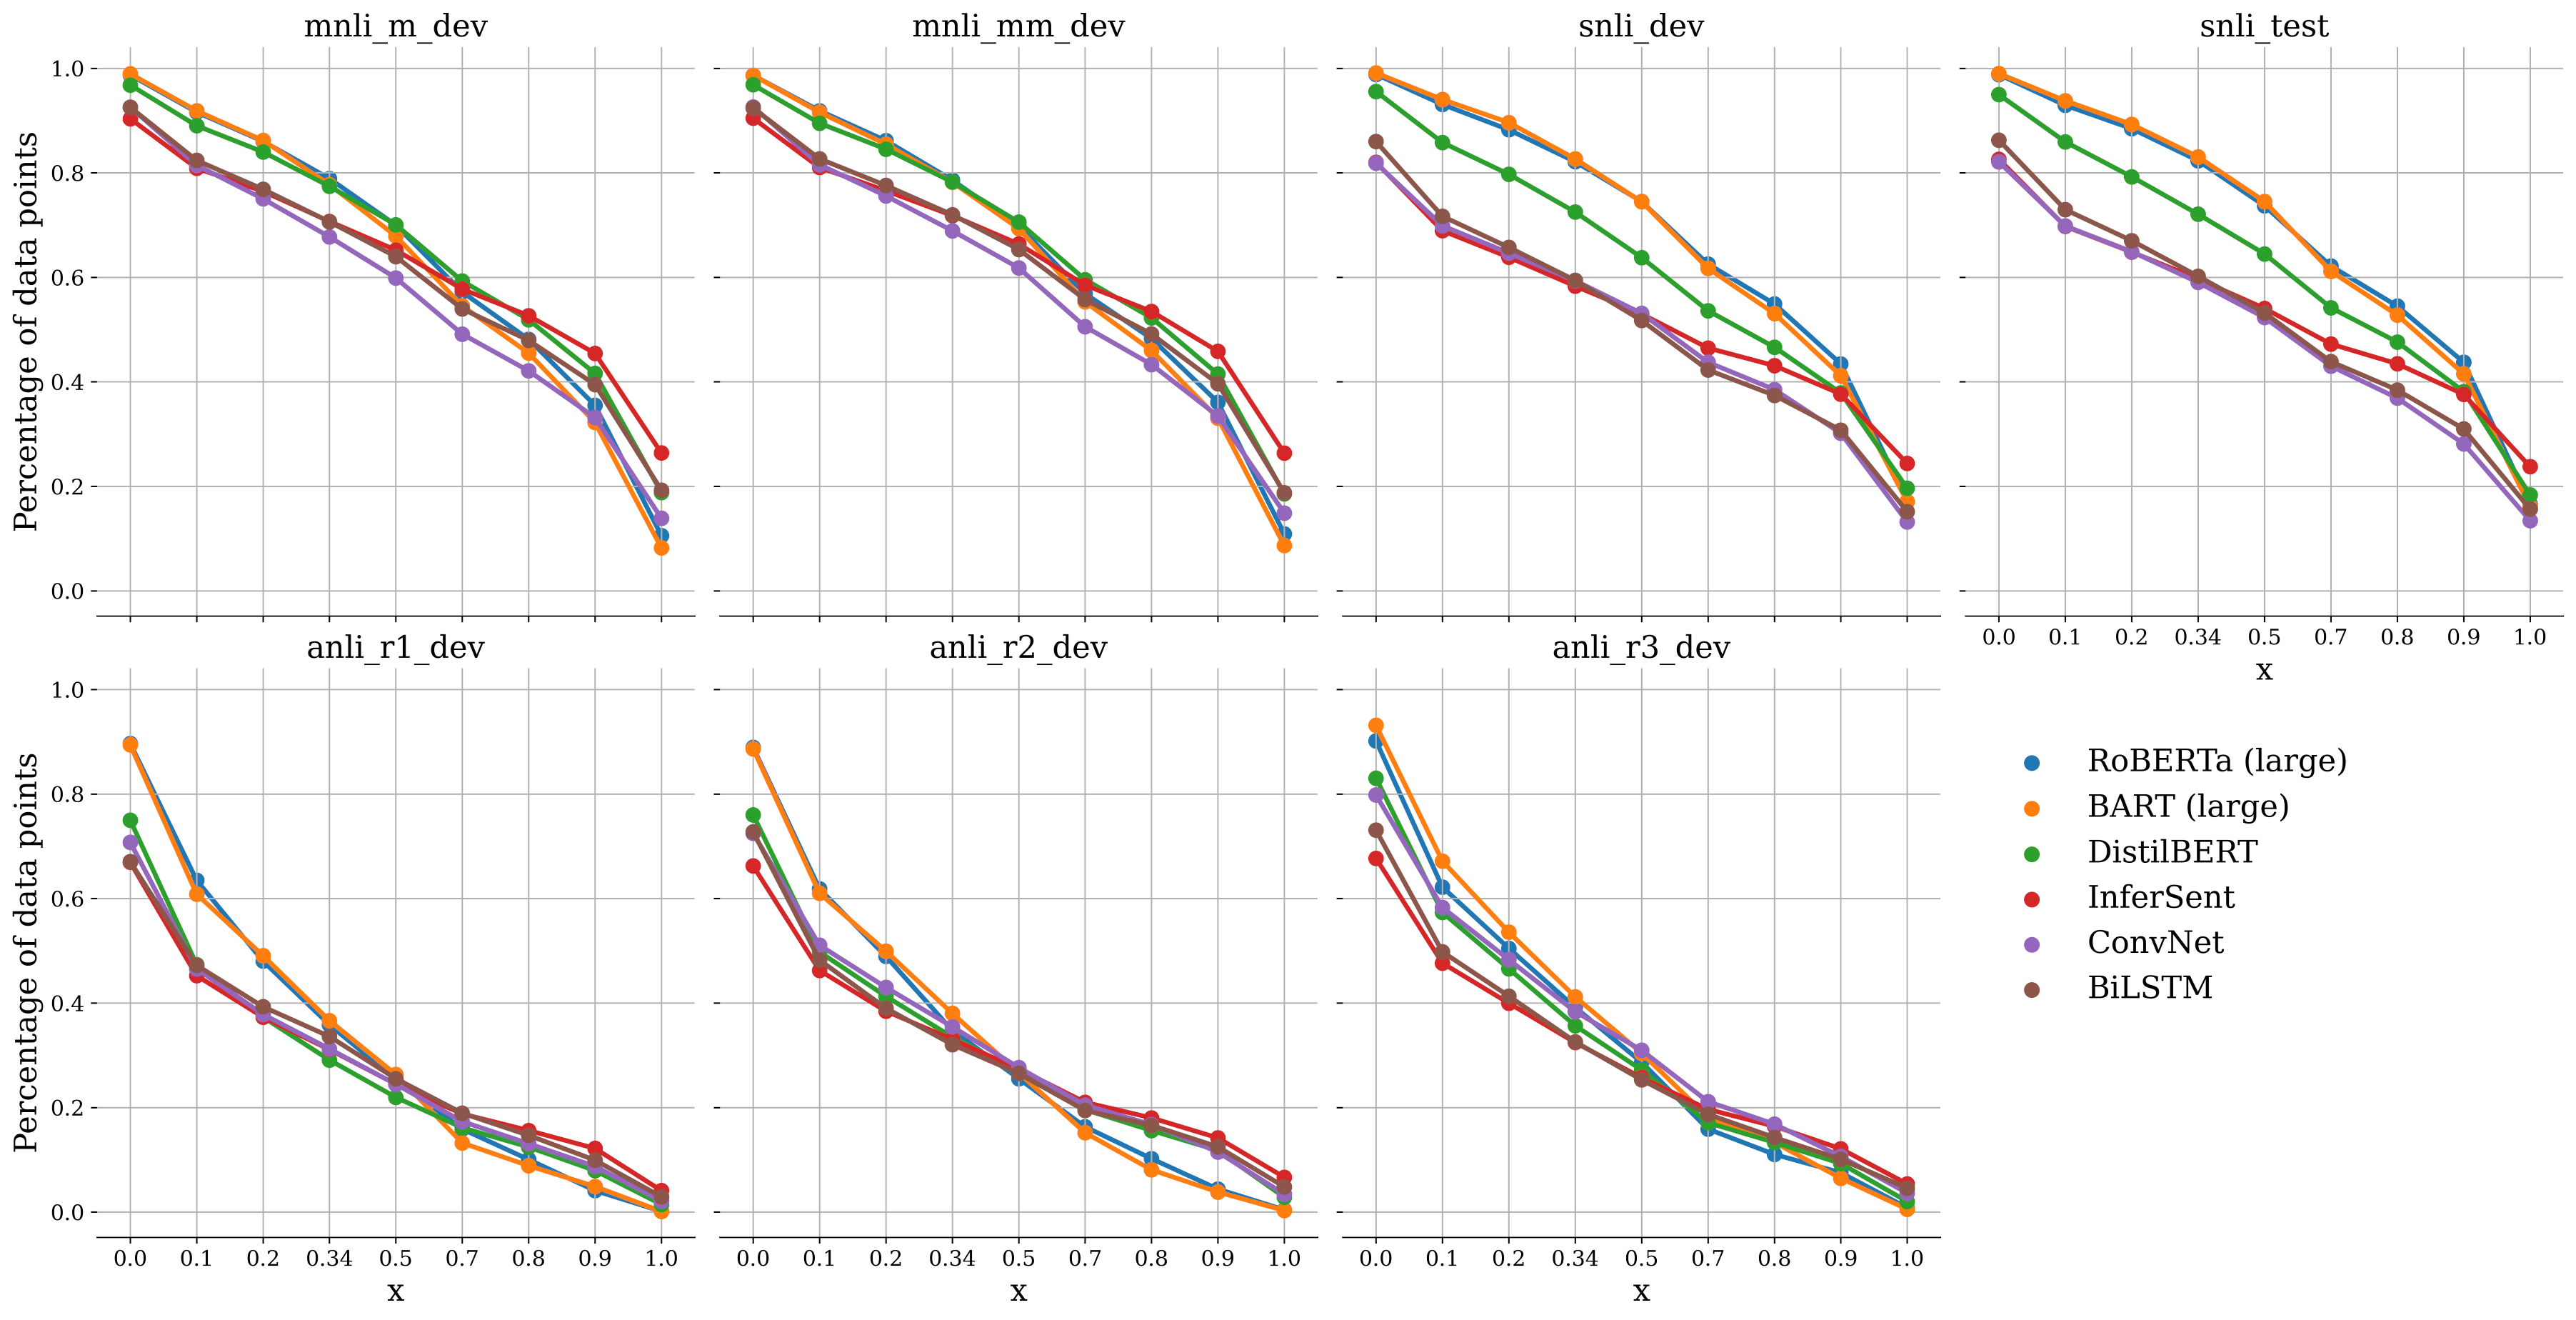
\includegraphics{figs/unli/omega_threshold.png}}
    \caption{$\Omega_x$ threshold for all datasets with varying $x$ and computing the percentage of examples that fall within the threshold. The top row consists of in-distribution datasets (MNLI, SNLI) and the bottom row contains out-of-distribution datasets (ANLI)}
    \label{fig:unli:threshold_omega_x}
\end{figure*}


We defined two variations of $\Omega_x$, $\Omega_{\text{max}}$ and $\Omega_{\text{rand}}$, but theoretically it is possible to define any arbitrary threshold percentage $x$ to evaluate the unnatural language inference mechanisms of different models. In \autoref{fig:unli:threshold_omega_x} we show the effect of different thresholds, including $\Omega_{\text{max}}$ where $x = 1/|D_{\text{test}|}$ and $\Omega_{\text{rand}}$ where $x = 0.34$. We observe for in-distribution datasets (top row, MNLI and SNLI splits), in the extreme setting when $x=1.0$, there are more than 10\% of examples available, and more than 25\% in case of InferSent and DistilBERT. For out-of-distribution datasets (bottom row, ANLI splits) we observe a much lower trend, suggesting generalization itself is the bottleneck in permuted sentence understanding.



\subsection{Models are very confident.}
\label{sec:unli_results_conf}

% Will it be too small?
\begin{figure}[t]
    \centering
    \resizebox{0.7\textwidth}{!}{
        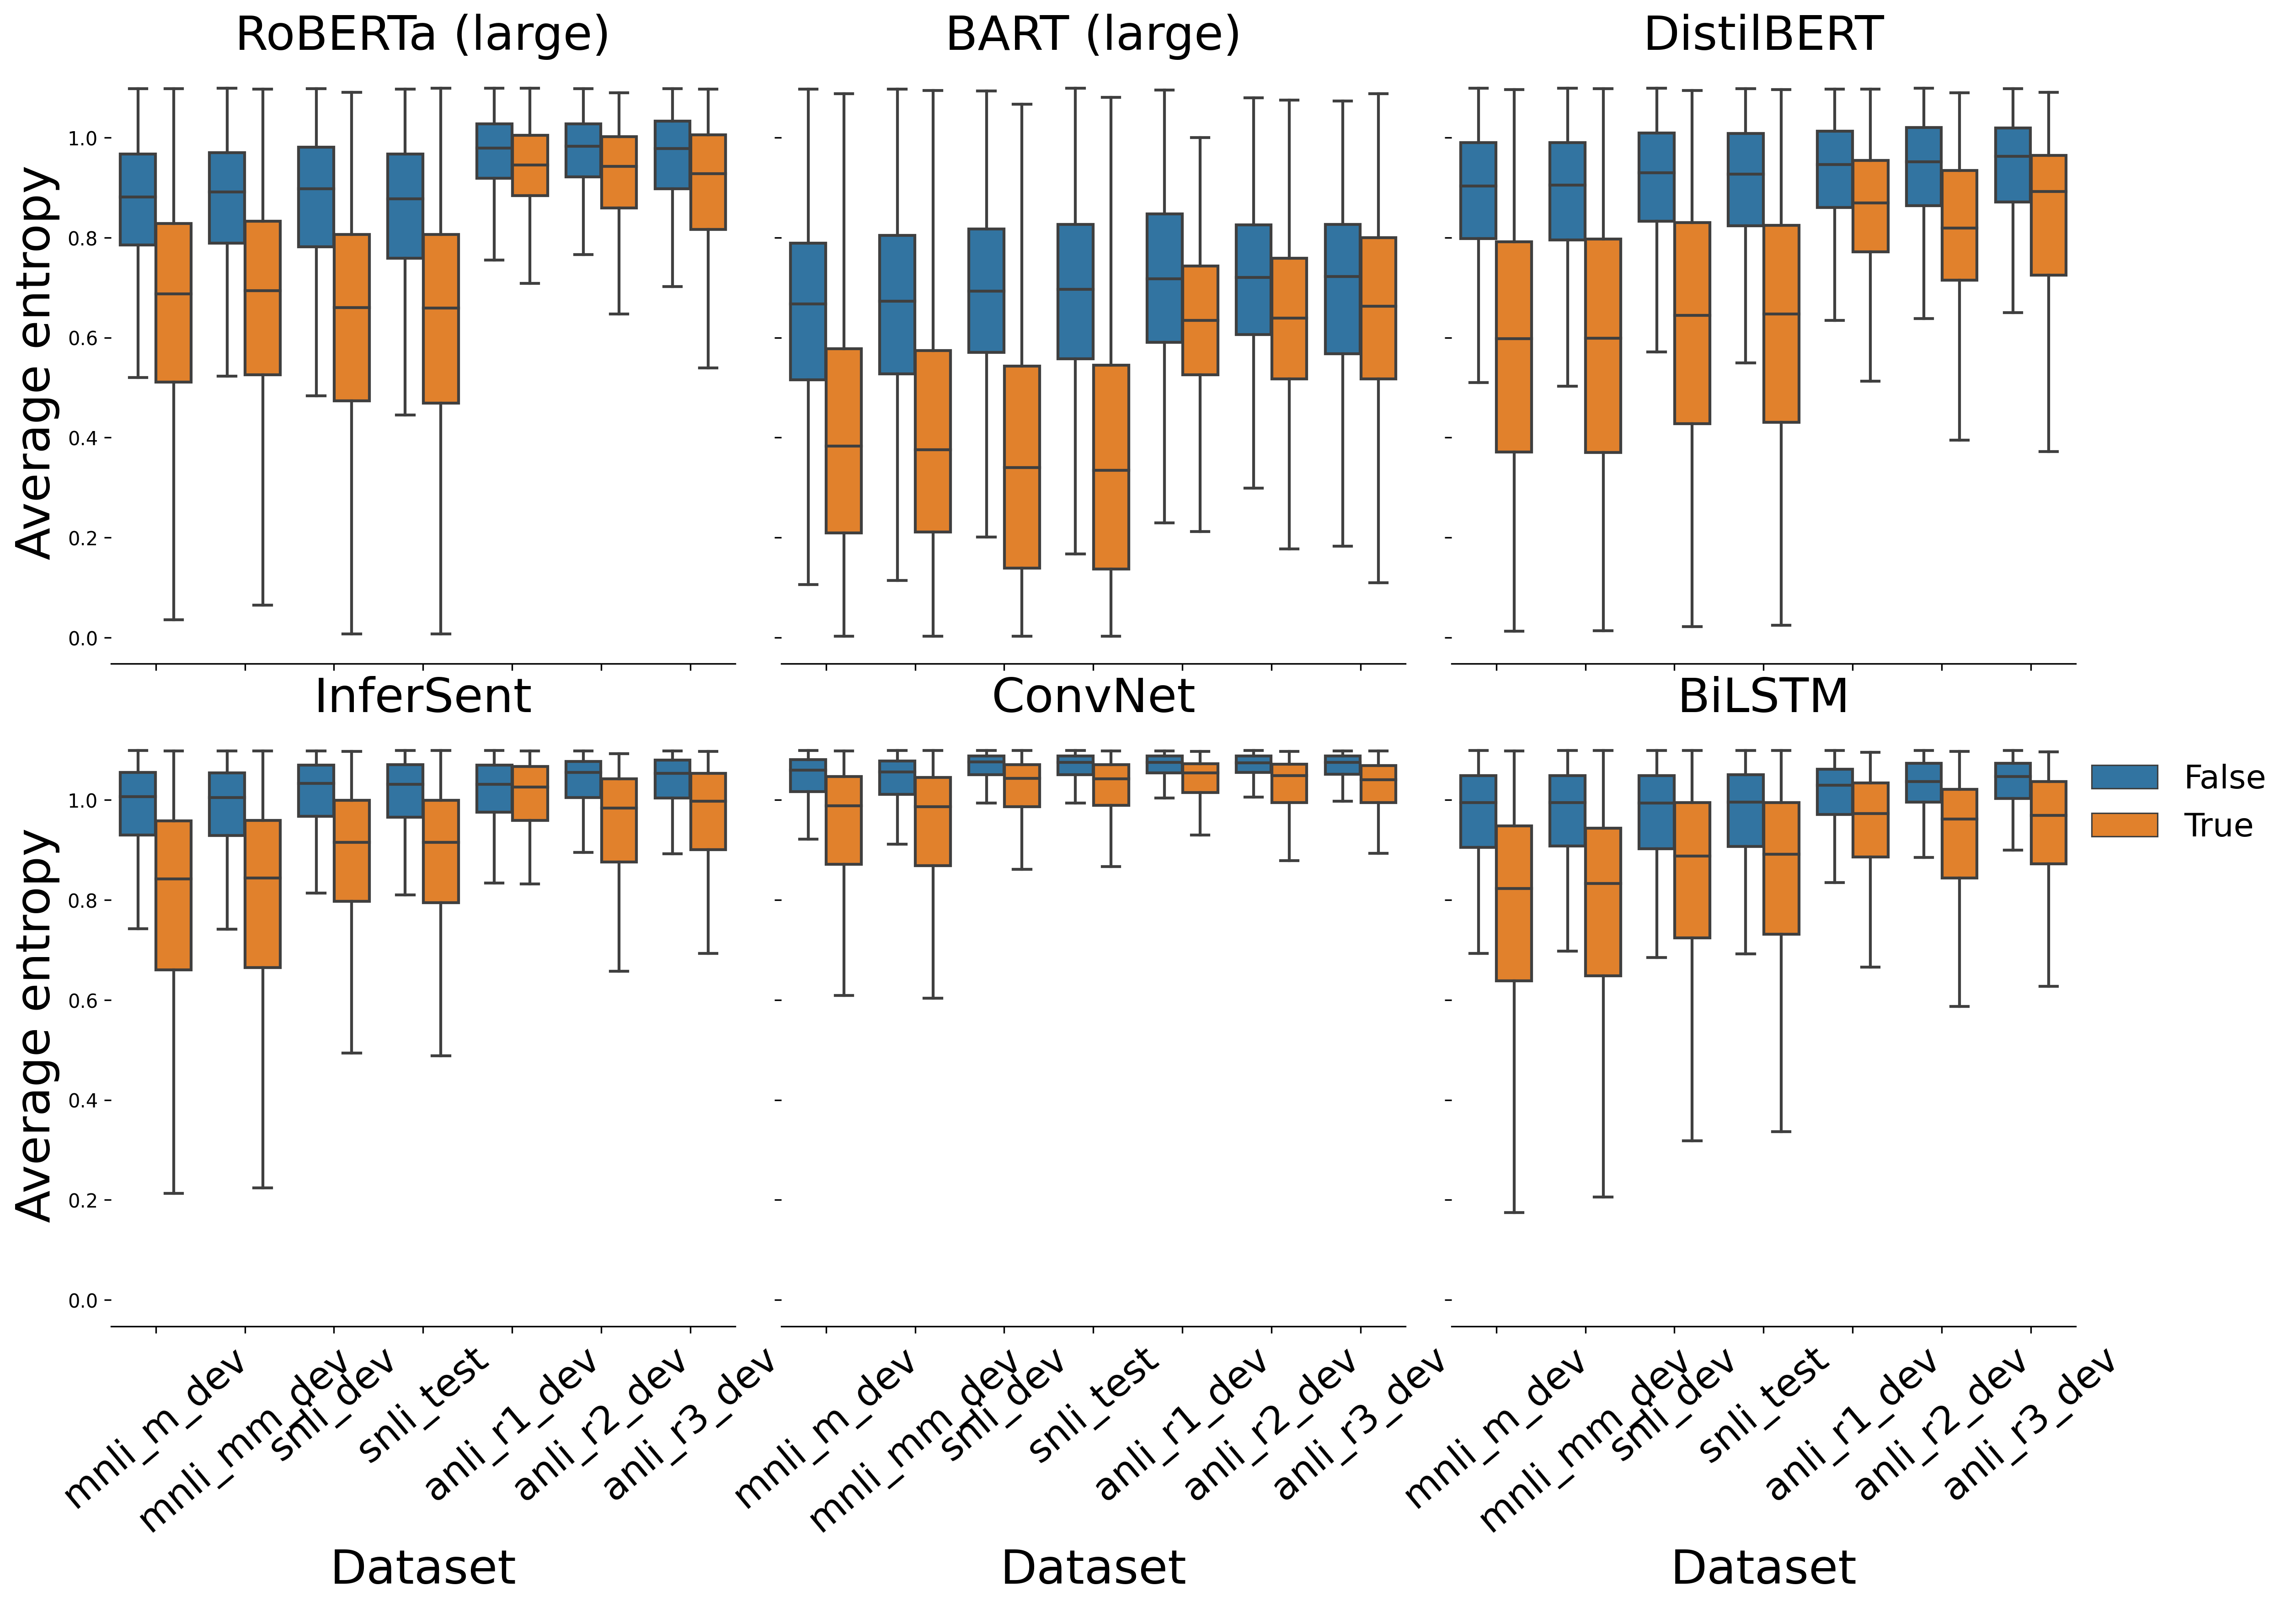
\includegraphics{figs/unli/entropy_plot.png}}
    \caption{Average entropy of model confidences on permutations that yielded the correct results for Transformer-based models (top) and Non-Transformer-based models (bottom). Results are shown for $D^c$ (orange) and $D^f$ (blue). The boxes show the quartiles of the entropy distributions.}
    \label{fig:unli_all_entropy}
\end{figure}


The phenomenon we observe would be of less concern if the correct label prediction was just an outcome of chance, which could occur when the entropy of the log probabilities of the model output is high (suggesting uniform probabilities on entailment, neutral and contradiction labels, recall Model B from \autoref{sec:unli_technical_bg}). We first investigate the model probabilities for the Transformer-based models on the permutations that lead to the correct answer in \autoref{fig:unli_all_entropy}. We find overwhelming evidence that model confidences on in-distribution datasets (MNLI, SNLI) are highly skewed, resulting in low entropy, and it varies among different model types. BART proves to be the most skewed Transformer-based model. This skewness is not a property of model capacity, as we observe DistilBERT log probabilities to have similar skewness as RoBERTa (large) model, while exhibiting lower $\mathcal{A}$, $\Omega_{\text{max}}$, and $\Omega_{\text{rand}}$.

% KS: I think this paper has the inverse result!
% The high confidence of Transformer-based model can be attributed to their tendency to be mis-calibrated in an out-of-domain setting, which is opposite to \newcite{desai2020calibration}!!!.

% [CHECK] comment on why Transformers are more confident. Find citations
% Do we know of a paper which shows Transformer entropies are low?
% Use the term calibration
% https://arxiv.org/pdf/2003.07892.pdf
% http://proceedings.mlr.press/v119/braverman20a/braverman20a.pdf

For non-Transformers whose accuracy $\mathcal{A}$ is lower, the $\Omega_{\text{max}}$ achieved by these models are also predictably lower. We observe roughly the same relative performance in the terms of $\Omega_{\text{max}}$ (\autoref{fig:comb_plot} and \autoref{table:unli_main}) and Average entropy (Figure \ref{fig:unli_all_entropy}). However, while comparing the averaged entropy of the model predictions, it is clear that there is some benefit to being a worse model---non-Transformer models are not as overconfident on randomized sentences as Transformers are.
High confidence of Transformer models can be attributed to the \textit{overthinking} phenomenon commonly observed in deep neural networks \cite{kaya2019shallowdeep} and BERT-based models \cite{zhou2020bert}.
% KS: I think this is a better reasoning? Please check.


\subsection{Similar artifacts in Chinese NLU.}
\label{sec:unli_ocnli_results}

\begin{table}[htbp]
    \centering
    \footnotesize
    \resizebox{0.7\linewidth}{!}{%
        \begin{tabular}{llrrrrrr}
            \toprule
             Model              & $\mathcal{A}$ & $\Omega_{\text{max}}$ & $\mathcal{P}^c$ & $\mathcal{P}^f$ & $\Omega_{\text{rand}}$ \\ \midrule
             RoBERTa-Large   & \textbf{0.784} &         \boldred{0.988} &                  0.726 &             \boldred{0.339} &                        \boldred{0.773}            \\
             InferSent &             0.573 &         0.931 &                  0.771 &             0.265 &                        0.615 \\
   ConvNet &              0.407 &         0.752 &                  \boldred{0.808} &             0.199 &                        0.426 \\
    BiLSTM &              0.566 &         0.963 &                  0.701 &             0.271 &                        0.611 \\
            \bottomrule
        \end{tabular}}
    \caption{Results on evaluation on OCNLI Dev set. All models are trained on OCNLI corpus \cite{hu-etal-2020-ocnli}. 
    % Max accuracy ($\Omega_{\text{max}}$) is computed based on whether \textit{any} of the $n=100$ permutations per data point yield correct results. $\mathcal{P}^c$  stands for the mean number of permutations which were correct when the original prediction is correct. $\mathcal{P}^f$  stats for the mean number of permutations which are correct when the original prediction is incorrect (flip). 
    Bold marks the highest value per metric (\boldred{red} shows the model is insensitive to permutation).}
    \label{table:ocnli_all}
\end{table}


We extended the experiments to the Original Chinese NLI dataset \citep[OCNLI]{hu-etal-2020-ocnli}, and re-used the pre-trained RoBERTa-Large and InferSent (non-Transformer) models on OCNLI. Our findings are similar to the English results (\autoref{table:ocnli_all}), thereby suggesting that the phenomenon is not just an artifact of English text or tokenization.

\subsection{Other Results.} We investigated the effect of sentence length (which correlates with number of possible permutations), and hypothesis-only randomization (models exhibit similar phenomenon even when only hypothesis is permuted). In terms of sentence length, we observe that shorter sentences in general have a somewhat higher probability of acceptance for examples which was originally predicted correctly---since shorter sentences have fewer unique permutations (\autoref{fig:unli_length}). However, for the examples which were originally incorrect, the trend is not present.

\begin{figure}[ht]
    \centering
    \resizebox{0.8\textwidth}{!}{
      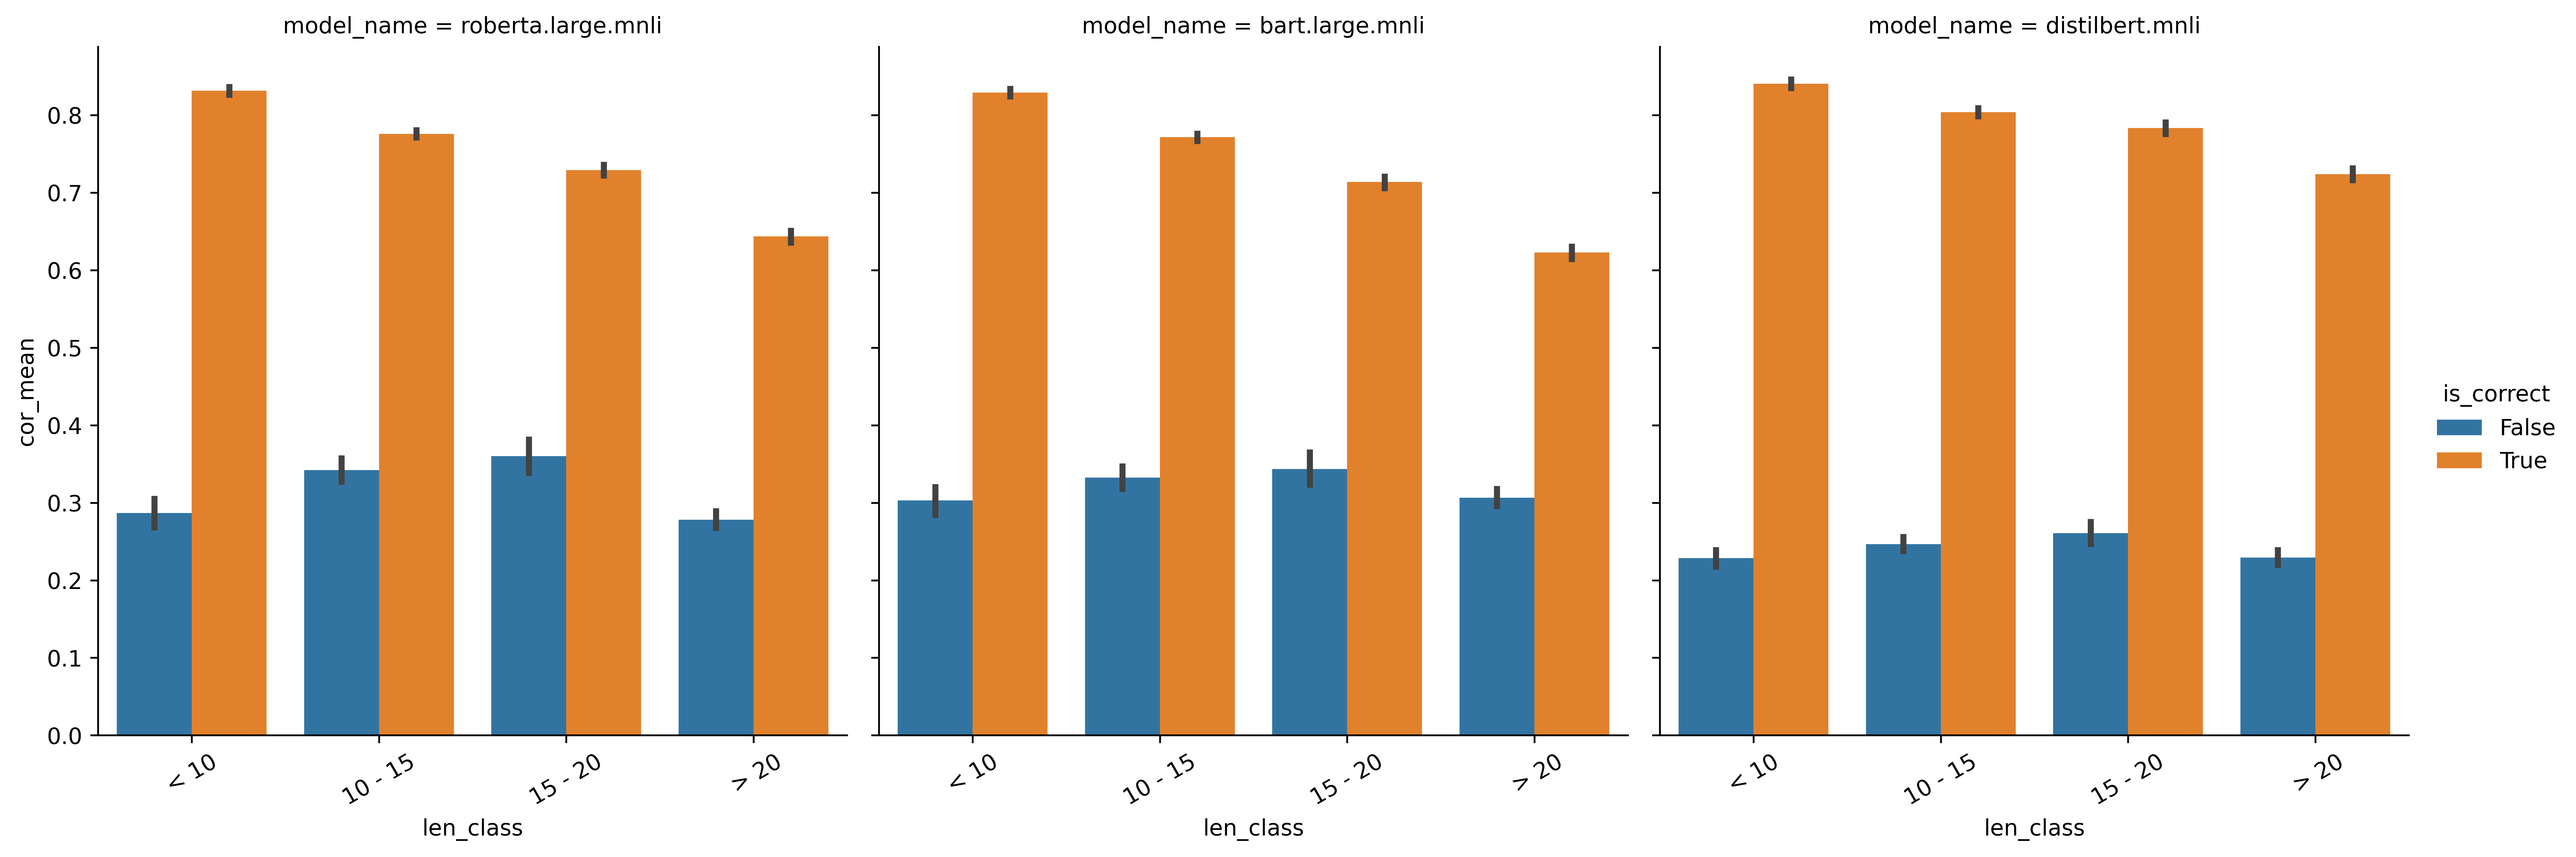
\includegraphics{figs/unli/transformer_length.png}
      % \includegraphics{example-image-a}
    }
    \caption{Length and \PermAcc by Transformer-based models.}
    \label{fig:unli_length}
\end{figure}

\begin{figure}[ht]
    \centering
    \resizebox{0.7\textwidth}{!}{
      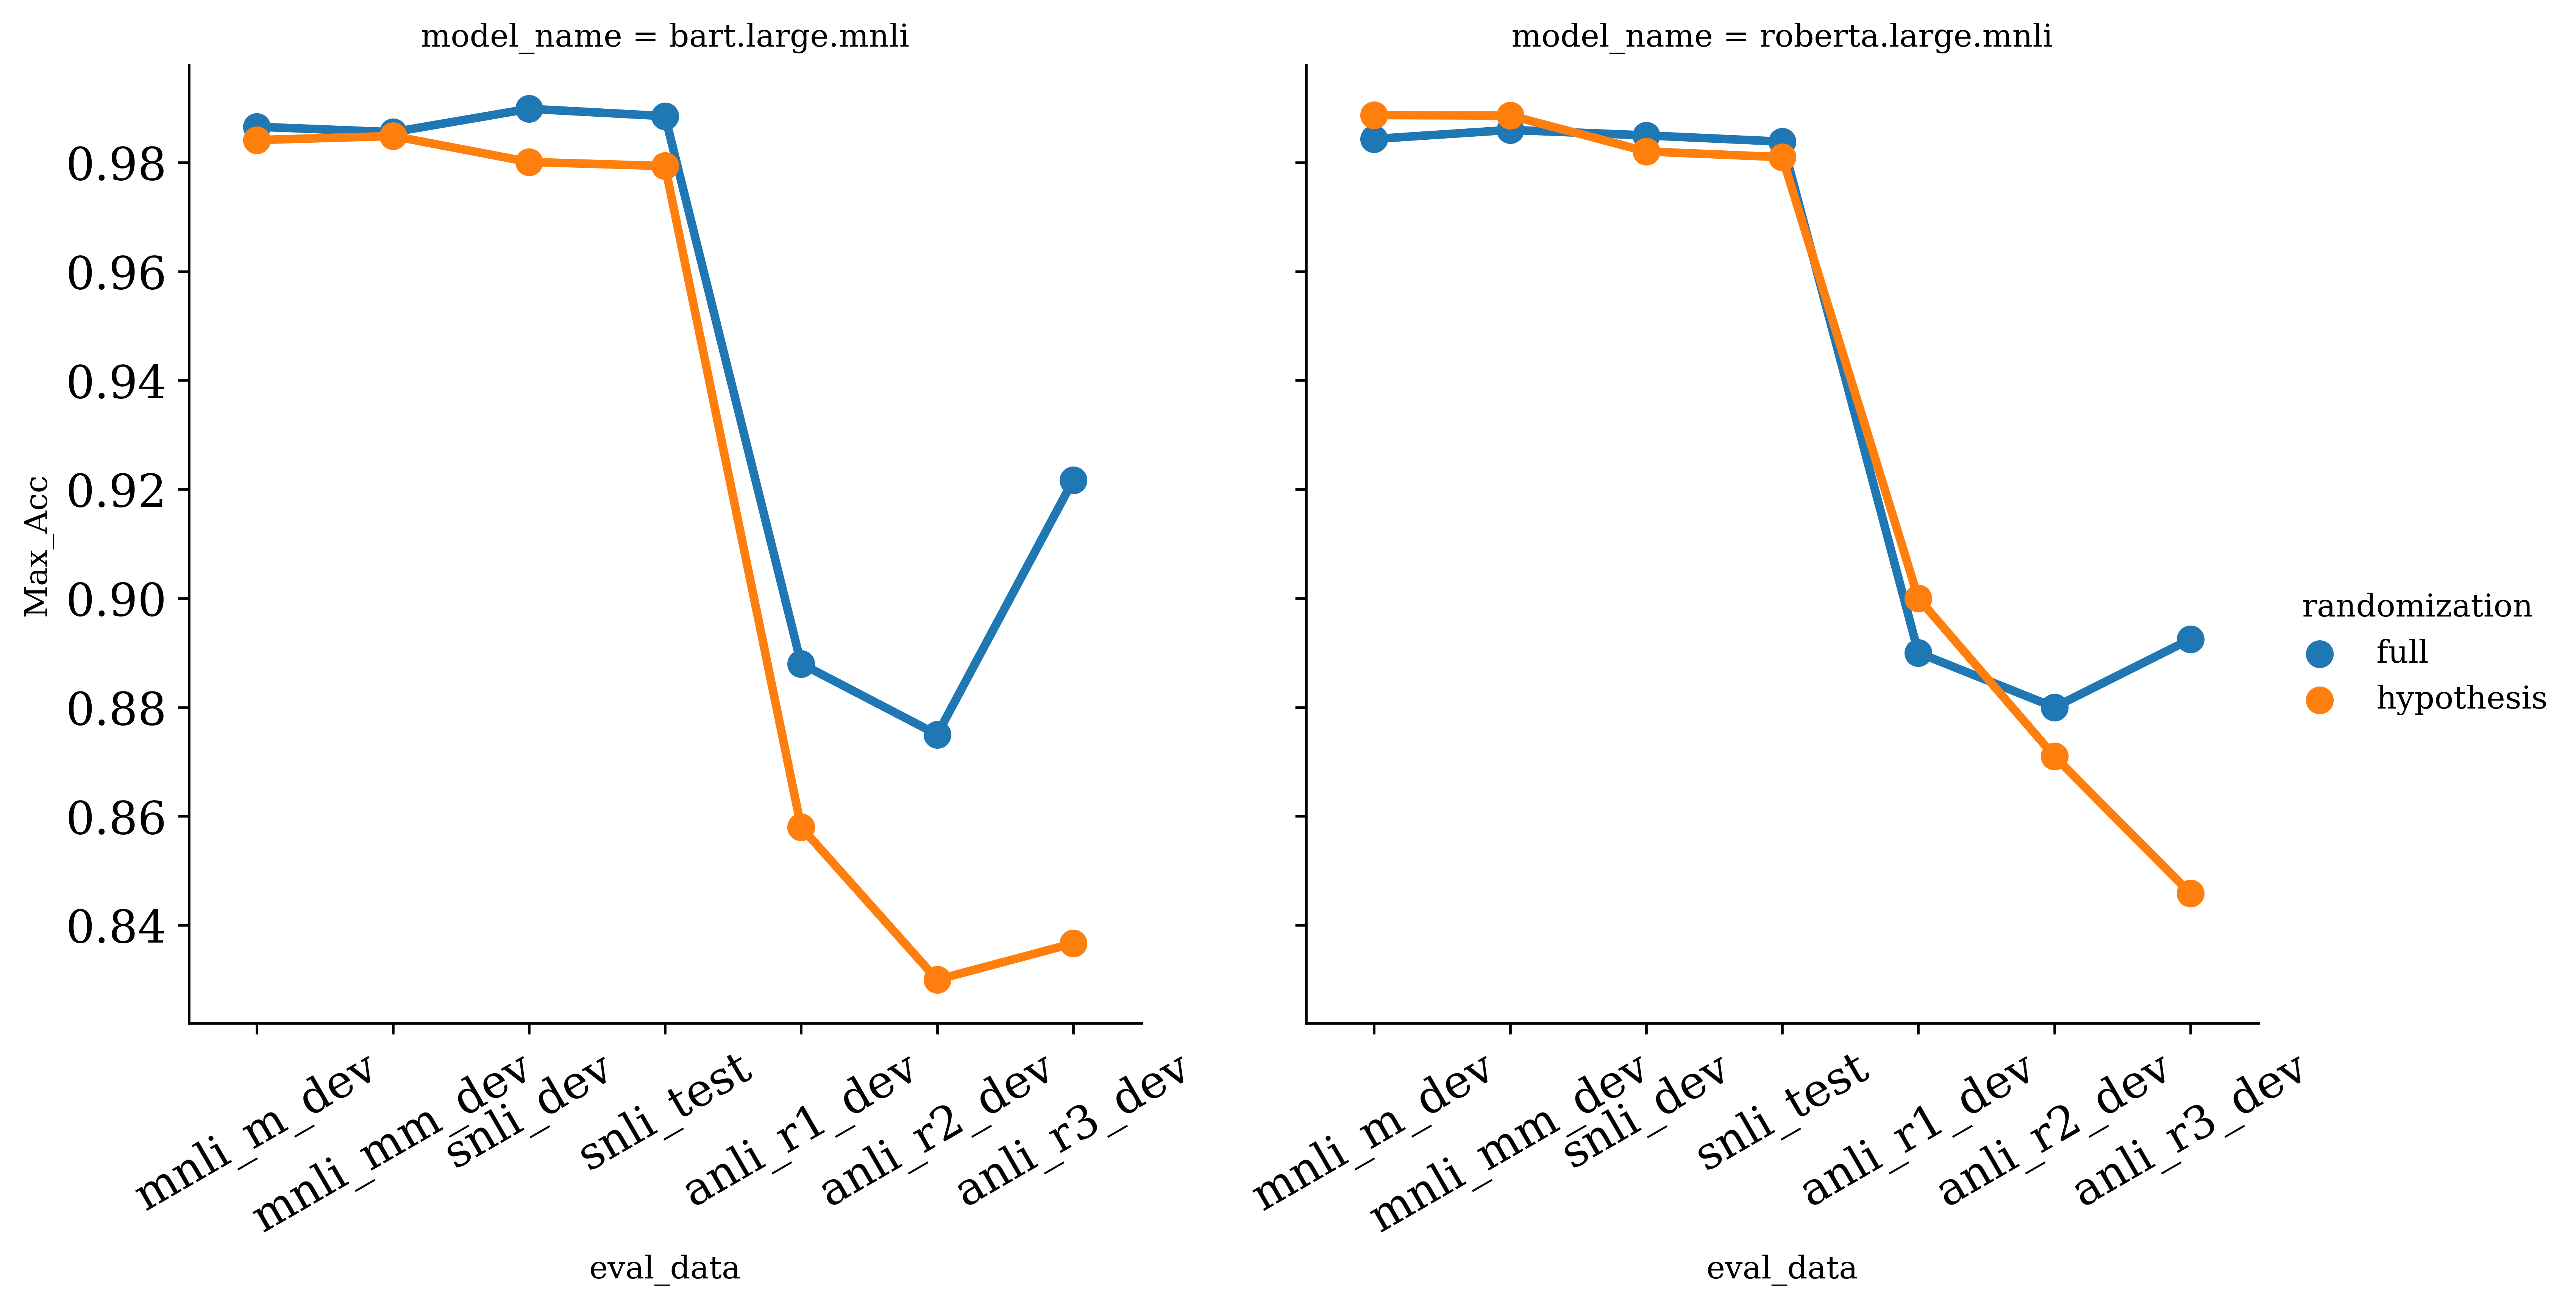
\includegraphics{figs/unli/hypothesis_compare.png}
    }
    \caption{Comparing the effect between randomizing both premise and hypothesis and only hypothesis on two Transformer-based models, RoBERTa and BART. Here, we observe the difference of $\Omega_{\text{max}}$ is marginal in in-distribution datasets (SNLI, MNLI), while hypothesis-only randomization is worse for out-of-distribution datasets (ANLI).}
    \label{fig:unli_hp_compare}
\end{figure}

\begin{figure}[ht]
  \centering
    \resizebox{0.7\textwidth}{!}{
      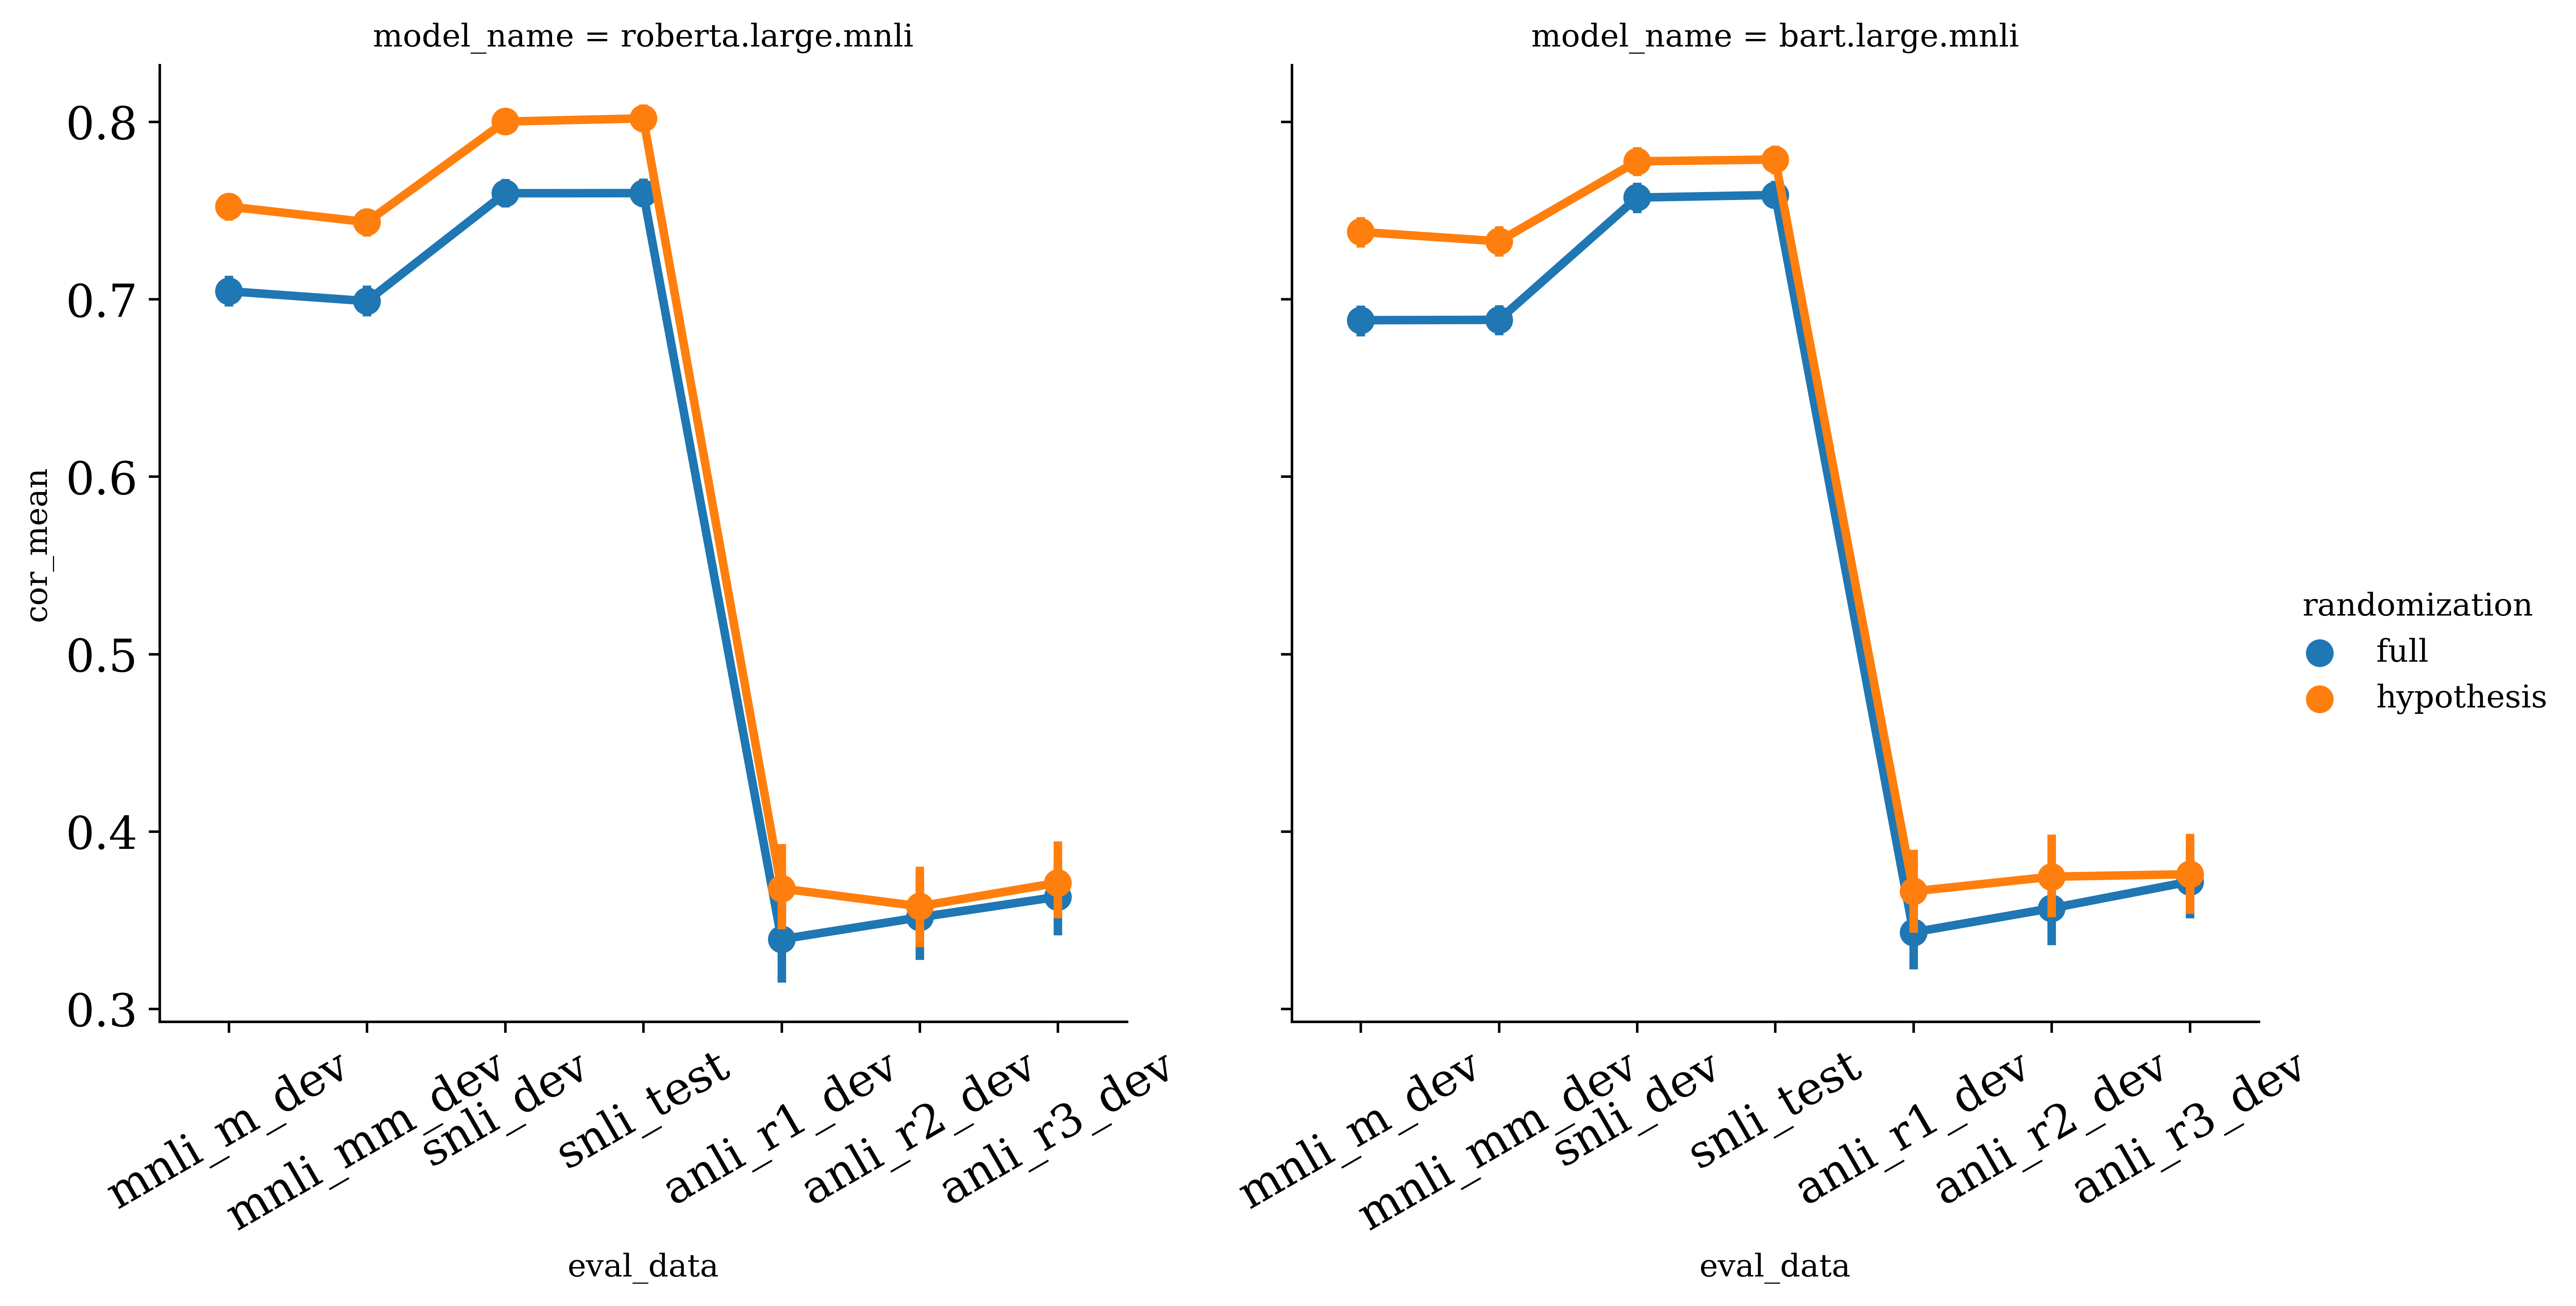
\includegraphics{figs/unli/hypothesis_compare_cor_mean.png}
      % \includegraphics{example-image-c}
    }
    \caption{Comparing the effect between randomizing both premise and hypothesis and only hypothesis on two Transformer-based models, RoBERTa and BART. In this figure, we compare the mean number of permutations which elicited correct response, and naturally the hypothesis-only randomization causes more percentage of randomizations to be correct.}
    \label{fig:unli_hp_compare_cor}
\end{figure}


In recent years, the impact of the hypothesis sentence \citep{gururangan-etal-2018-annotation, tsuchiya-2018-performance, poliak-etal-2018-hypothesis} on NLI classification has been a topic of much interest. As we define in \autoref{sec:unli_technical_bg}, logical entailment can only be defined for pairs of propositions. We investigated one effect where we randomize only the hypothesis sentences while keeping the premise intact. \autoref{fig:unli_hp_compare} and \autoref{fig:unli_hp_compare_cor} shows that the $\Omega_{\text{max}}$ value is almost the same for the two schemes; randomizing the hypothesis alone also leads the model to accept many permutations.


\section{Analysis}

\subsection{Analyzing Syntactic Structure Associated with Tokens}
\label{sec:unli_pos_mini_tree}


\begin{figure}[t]
    \centering
    \resizebox{0.48\textwidth}{!}{
        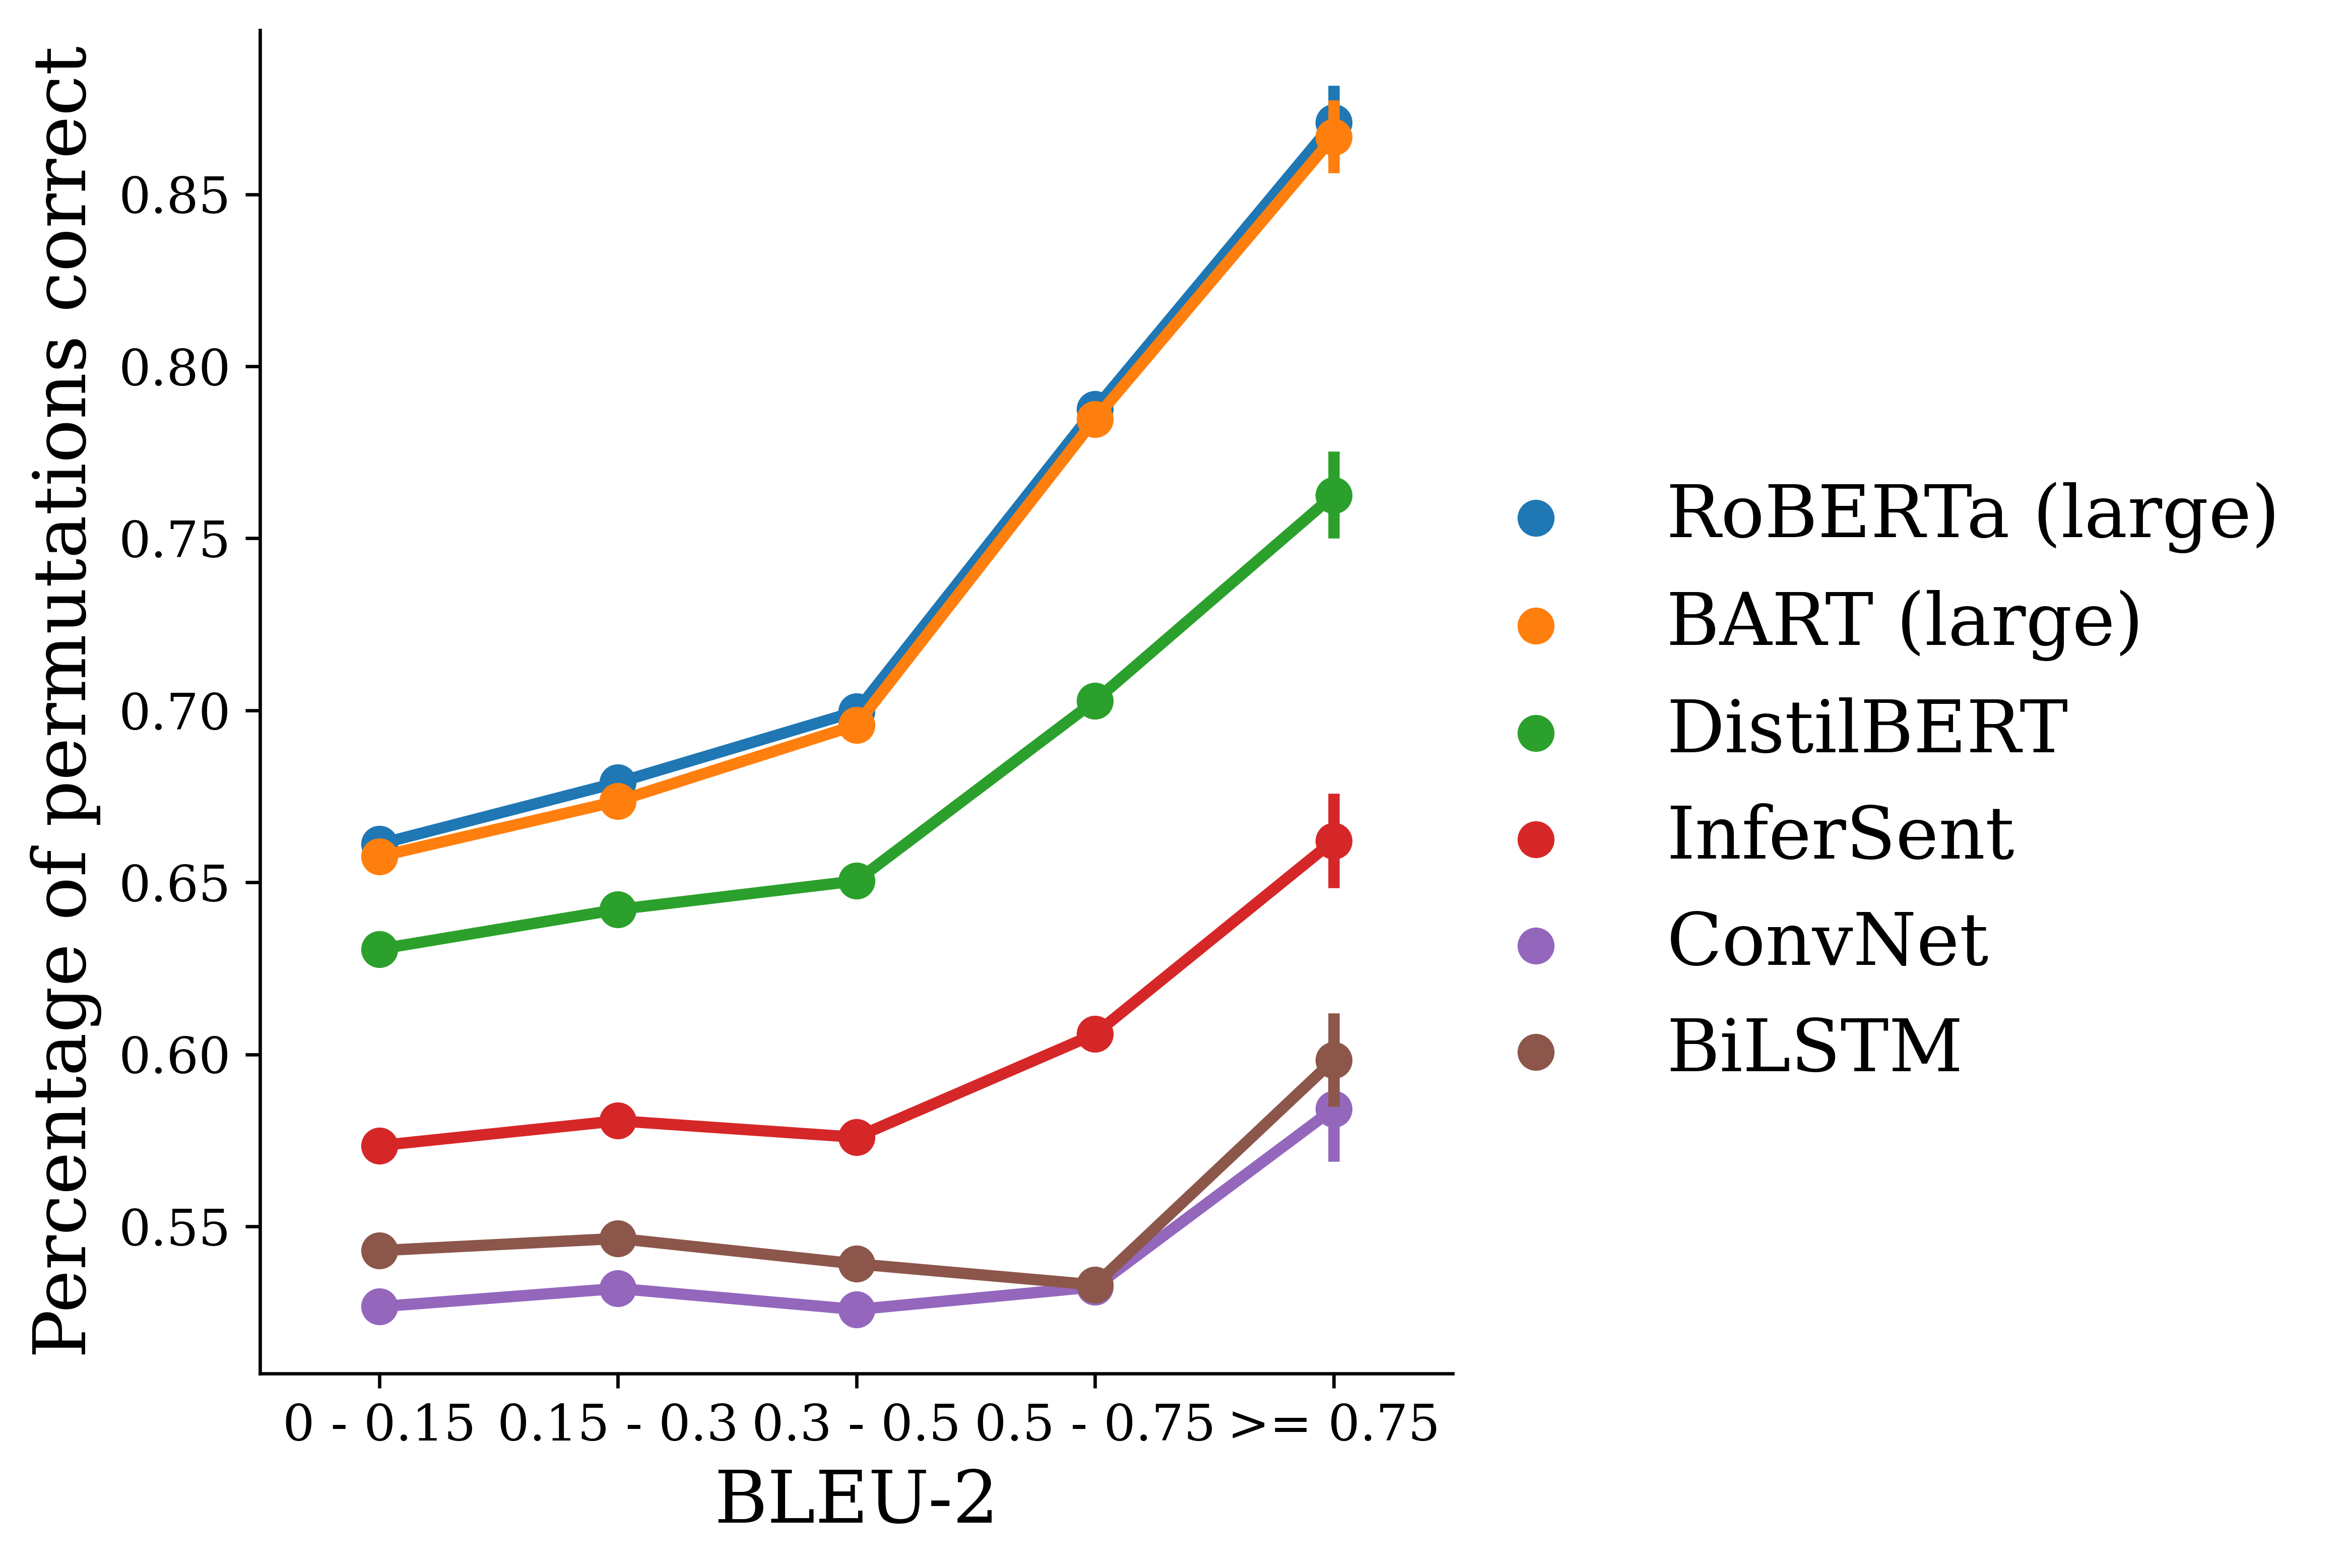
\includegraphics{figs/unli/bleu_2_all.png}}
    \caption{BLEU-2 score versus acceptability of permuted sentences across all test datasets. RoBERTa and BART performance is similar but differs considerably from the performance of non-Transformer-based models, such as InferSent and ConvNet. }
    \label{fig:bleu_2}
\end{figure}

A natural question to ask following our findings: what is it about particular permutations that leads models to accept them? Since the permutation operation is drastic and only rarely preserves local word relations, we first investigate whether there exists a relationship between \PermAcc\ scores and local word order preservation. Concretely, we compare bi-gram word overlap (BLEU-2) with the percentage of permutations that are deemed correct (\autoref{fig:bleu_2}).\footnote{We observe, due to our permutation process, the maximum BLEU-3 and BLEU-4 scores are negligibly low ($< 0.2$  BLEU-3 and $< 0.1$ BLEU-4), already calling into question the hypothesis that n-grams are the sole explanation for our finding. Because of this, we only compare BLEU-2 scores. Detailed experiments on specially constructed permutations that cover the entire range of BLEU-3 and BLEU-4 is provided in \autoref{app_sec:bleu_all}.} Although the probability of a permuted sentence to be predicted correctly does appear to track BLEU-2 score (Figure \ref{fig:bleu_2}), the percentage of examples which were assigned the gold label by the Transformer-based models is still higher than we would expect from permutations with lower BLEU-2 (66\% for the lowest BLEU-2 range of $0-0.15$), suggesting preserved relative word order alone cannot explain the high permutation acceptance rates.

Thus, we find that local order preservation does correlate with \PermAcc, but it doesn't fully explain the high \PermAcc\ scores.
We now further ask whether $\Omega$ is related to a more abstract measure of local word relations, i.e., part-of-speech (POS) neighborhood.

%We perform two initial analyses to shed light on this question. First, we ask whether \PermAcc\ scores are higher when local word order is preserved?
%We might expect this to be the case if the models memorize words along with their local neighbors. %does this clarify the point?
%We find that local order preservation does correlate with \PermAcc, but it doesn't fully explain the high \PermAcc\ scores. Second, we ask whether $\Omega$ is related to a more abstract measure of local word relations, i.e., part-of-speech (POS) neighborhood. We find that there is little effect of POS-neighbors for non-Transformer models, but that RoBERTa, BART, and DistilBERT show a distinct effect. Taken together these analyses suggest that some local word order information affects models' \PermAcc\ scores, and perhaps incorporating methods of decreasing model reliance on this information could be fruitful.

%\paragraph{Preserving Local Word Order Leads to Higher \PermAcc.}

%Although we constrained our randomization such that no word appears in its original position, we didn't impose any restrictions on the relative positions of n-grams. To investigate the extent to which relative n-gram order is preserved, we compare 2-, 3- and 4 n-gram BLEU scores \citep{papineni-etal-2002-bleu} to the $\Omega$ values across models.
%If preserved n-grams are driving the \PermAcc\ effects, we should low $\Omega$ values for examples with low BLEU and high $\Omega$ for examples with high BLEU. % didn't understand this part
%As a result of our permutation process, the maximum BLEU-3 and BLEU-4 scores are negligibly low ($< 0.2$  BLEU-3 and $< 0.1$ BLEU-4), already calling into question the hypothesis that n-grams are the sole explanation for our finding. Because of this, we only compare BLEU-2 scores. (Detailed experiments on specially constructed permutations that cover the entire range of BLEU-3 and BLEU-4 is provided in \autoref{app_sec:bleu_all}). Although the probability of a permuted sentence to be predicted correctly does correlate with BLEU-2 score (Figure \ref{fig:bleu_2}), the percentage of examples predicted correct by Transformer-based models is still higher than we would expect from permutations with lower BLEU-2 (66\% for the lowest BLEU-2 range of $0-0.15$), suggesting preserved relative word order alone cannot explain the high permutation acceptance rates.



% \paragraph{Part-of-speech neighborhood tracks \PermAcc.}

Many syntactic formalisms, like Lexical Functional Grammar \citep[LFG]{kaplan-bresnan-1995-formal, bresnan-etal-2015-lexical}, Head-drive Phrase Structure Grammar \citep[HPSG]{pollard-sag-1994-head} or Lexicalized Tree Adjoining Grammar \citep[LTAG]{schabes-etal-1988-parsing, abeille-1990-lexical}, are ``lexicalized'', i.e., individual words or morphemes bear syntactic features telling us which other words they can combine with. For example, ``buy'' could be associated with (at least) two lexicalized syntactic structures, one containing two noun phrases (as in \textit{\underline{Kim} bought \underline{cheese}}), and another with three (as in \textit{\underline{Lee} bought \underline{Logan} \underline{cheese}}). %In this way, an average tree family for any particular word, like \textit{buy}, can provide information about neighbors it often appears with. Taking inspiration from formalisms like this,
We speculate that our NLI models might accept permuted examples at high rates, %even when local n-gram orders aren't preserved,
because they are (perhaps noisily) reconstructing the original sentence from abstract, word-anchored information about common neighbors.

To test this, we POS-tagged $D_{\text{train}}$ using 17 Universal Part-of-Speech tags (using spaCy, \citealt{spacy2}). %For each token in $D_{\text{train}}$, we get a summary of that token's syntactic context (at a symmetrical distance set by a hyperparameter we call the \textbf{radius}). Concretely,
For each $w_i \in S_i$, we compute the occurrence probability of POS tags on tokens in the \textit{neighborhood} of $w_i$. The neighborhood is specified by the radius $r$ (a symmetrical window $r$ tokens from $w_i \in S_i$ to the left and right). We denote this sentence level probability of neighbor POS tags for a word $w_i$ as $\psi^r_{\{w_i, S_i\}} \in \mathcal{R}^{17}$. Sentence-level word POS neighbor scores can be averaged across $ D_{\text{train}}$ to get a type level score $\psi^r_{\{w_i, D_{\text{train}}\}} \in \mathcal{R}^{17}, \forall w_i \in D_{\text{train}}$.  Then, for a sentence $S_i \in D_{\text{test}}$, for each word $w_i \in S_i$, we compute a \textbf{POS mini-tree overlap score}:
%\begin{align}
\begin{equation} % want left align
\begin{split}
\beta^k_{\{w_i,S_i\}} =
\frac{1}{k} \mid \text{argmax}_k &\psi^r_{\{w_i, D_{\text{train}}\}} \cap \\ &\text{argmax}_k\psi^r_{\{w_i, S_i\}} \mid
\end{split}
\end{equation}
%\end{align}

% POS signature?
Concretely, $\beta^k_{\{w_i,S_i\}}$ computes the overlap of top-$k$ POS tags in the neighborhood of a word $w_i$ in $S$ with that of the train statistic. If a word has the same mini-tree in a given sentence as it has in the training set, then the overlap would be 1. For a given sentence $S_i$, the aggregate $\beta^k_{\{S_i\}}$ is defined by the average of the overlap scores of all its words: $\beta^k_{\{S_i\}} = \frac{1}{|S_i|}\sum_{w_i \in S_i} \beta^k_{\{w_i,S_i\}}$, and we call it a POS minitree \textit{signature}. We can also compute the POS minitree signature of a permuted sentence $\hat{S}_i$ to have $\beta^k_{\{\hat{S}_i\}}$.  If the permuted sentence POS signature comes close to that of the true sentence, then their ratio (i.e.,  $\beta^k_{\{\hat{S}_i\}} / \beta^k_{\{S_i\}}$) will be close to 1. Also, since POS signature is computed with respect to the train distribution, a ratio of $>$ 1 indicates that the permuted sentence is closer to the overall train statistic than to the original unpermuted sentence in terms of POS signature. %If models ``know syntax'' then for any samples (from the permuted test set or from the original training) that have high average (?) POS tag minitree overlap scores (i.e., words with POS tag minitree scores similar to their POS tag minitree overlap score on the training set), we should expect those samples to be fairly easy for models to do well on.
If high overlap with the training distribution correlates with percentage of permutations deemed correct, then our models treat words as if they project syntactic minitrees.
%Therefore, for $\hat{D}_{\text{test}}$ where many of the $n$ permutations have high average POS minitree overlap score, we should expect a higher prediction accuracy.
\autoref{fig:unli_pos_signature} provides a snapshot a word ``river" from the test set and shows how the POS signature distribution of the word in a particular example match with that of aggregated training statistic. In practice, we select the top $k$ POS tags for the word in the test signature as well as the train, and calculate their overlap. When comparing the model performance with permuted sentences, we compute a ratio between the original test overlap score and an overlap score calculated instead from the permuted test. In the \autoref{fig:unli_pos_signature}, `river' would have a POS tag minitree score of 0.75.

\begin{figure}[ht]
    \centering
    \resizebox{0.7\linewidth}{!}{
        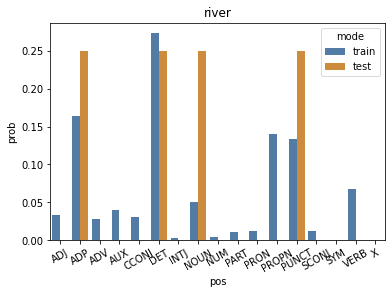
\includegraphics{figs/unli/riverPOSsig}}
    \caption{Example POS signature for the word `river', calculated with a radius of 2. Probability of each neighbor POS tag is provided. Orange examples come from the permuted test set, and blue come from the original training data. }
    \label{fig:unli_pos_signature}
\end{figure}



\begin{figure}[t]
    \centering
    \resizebox{0.6\linewidth}{!}{
        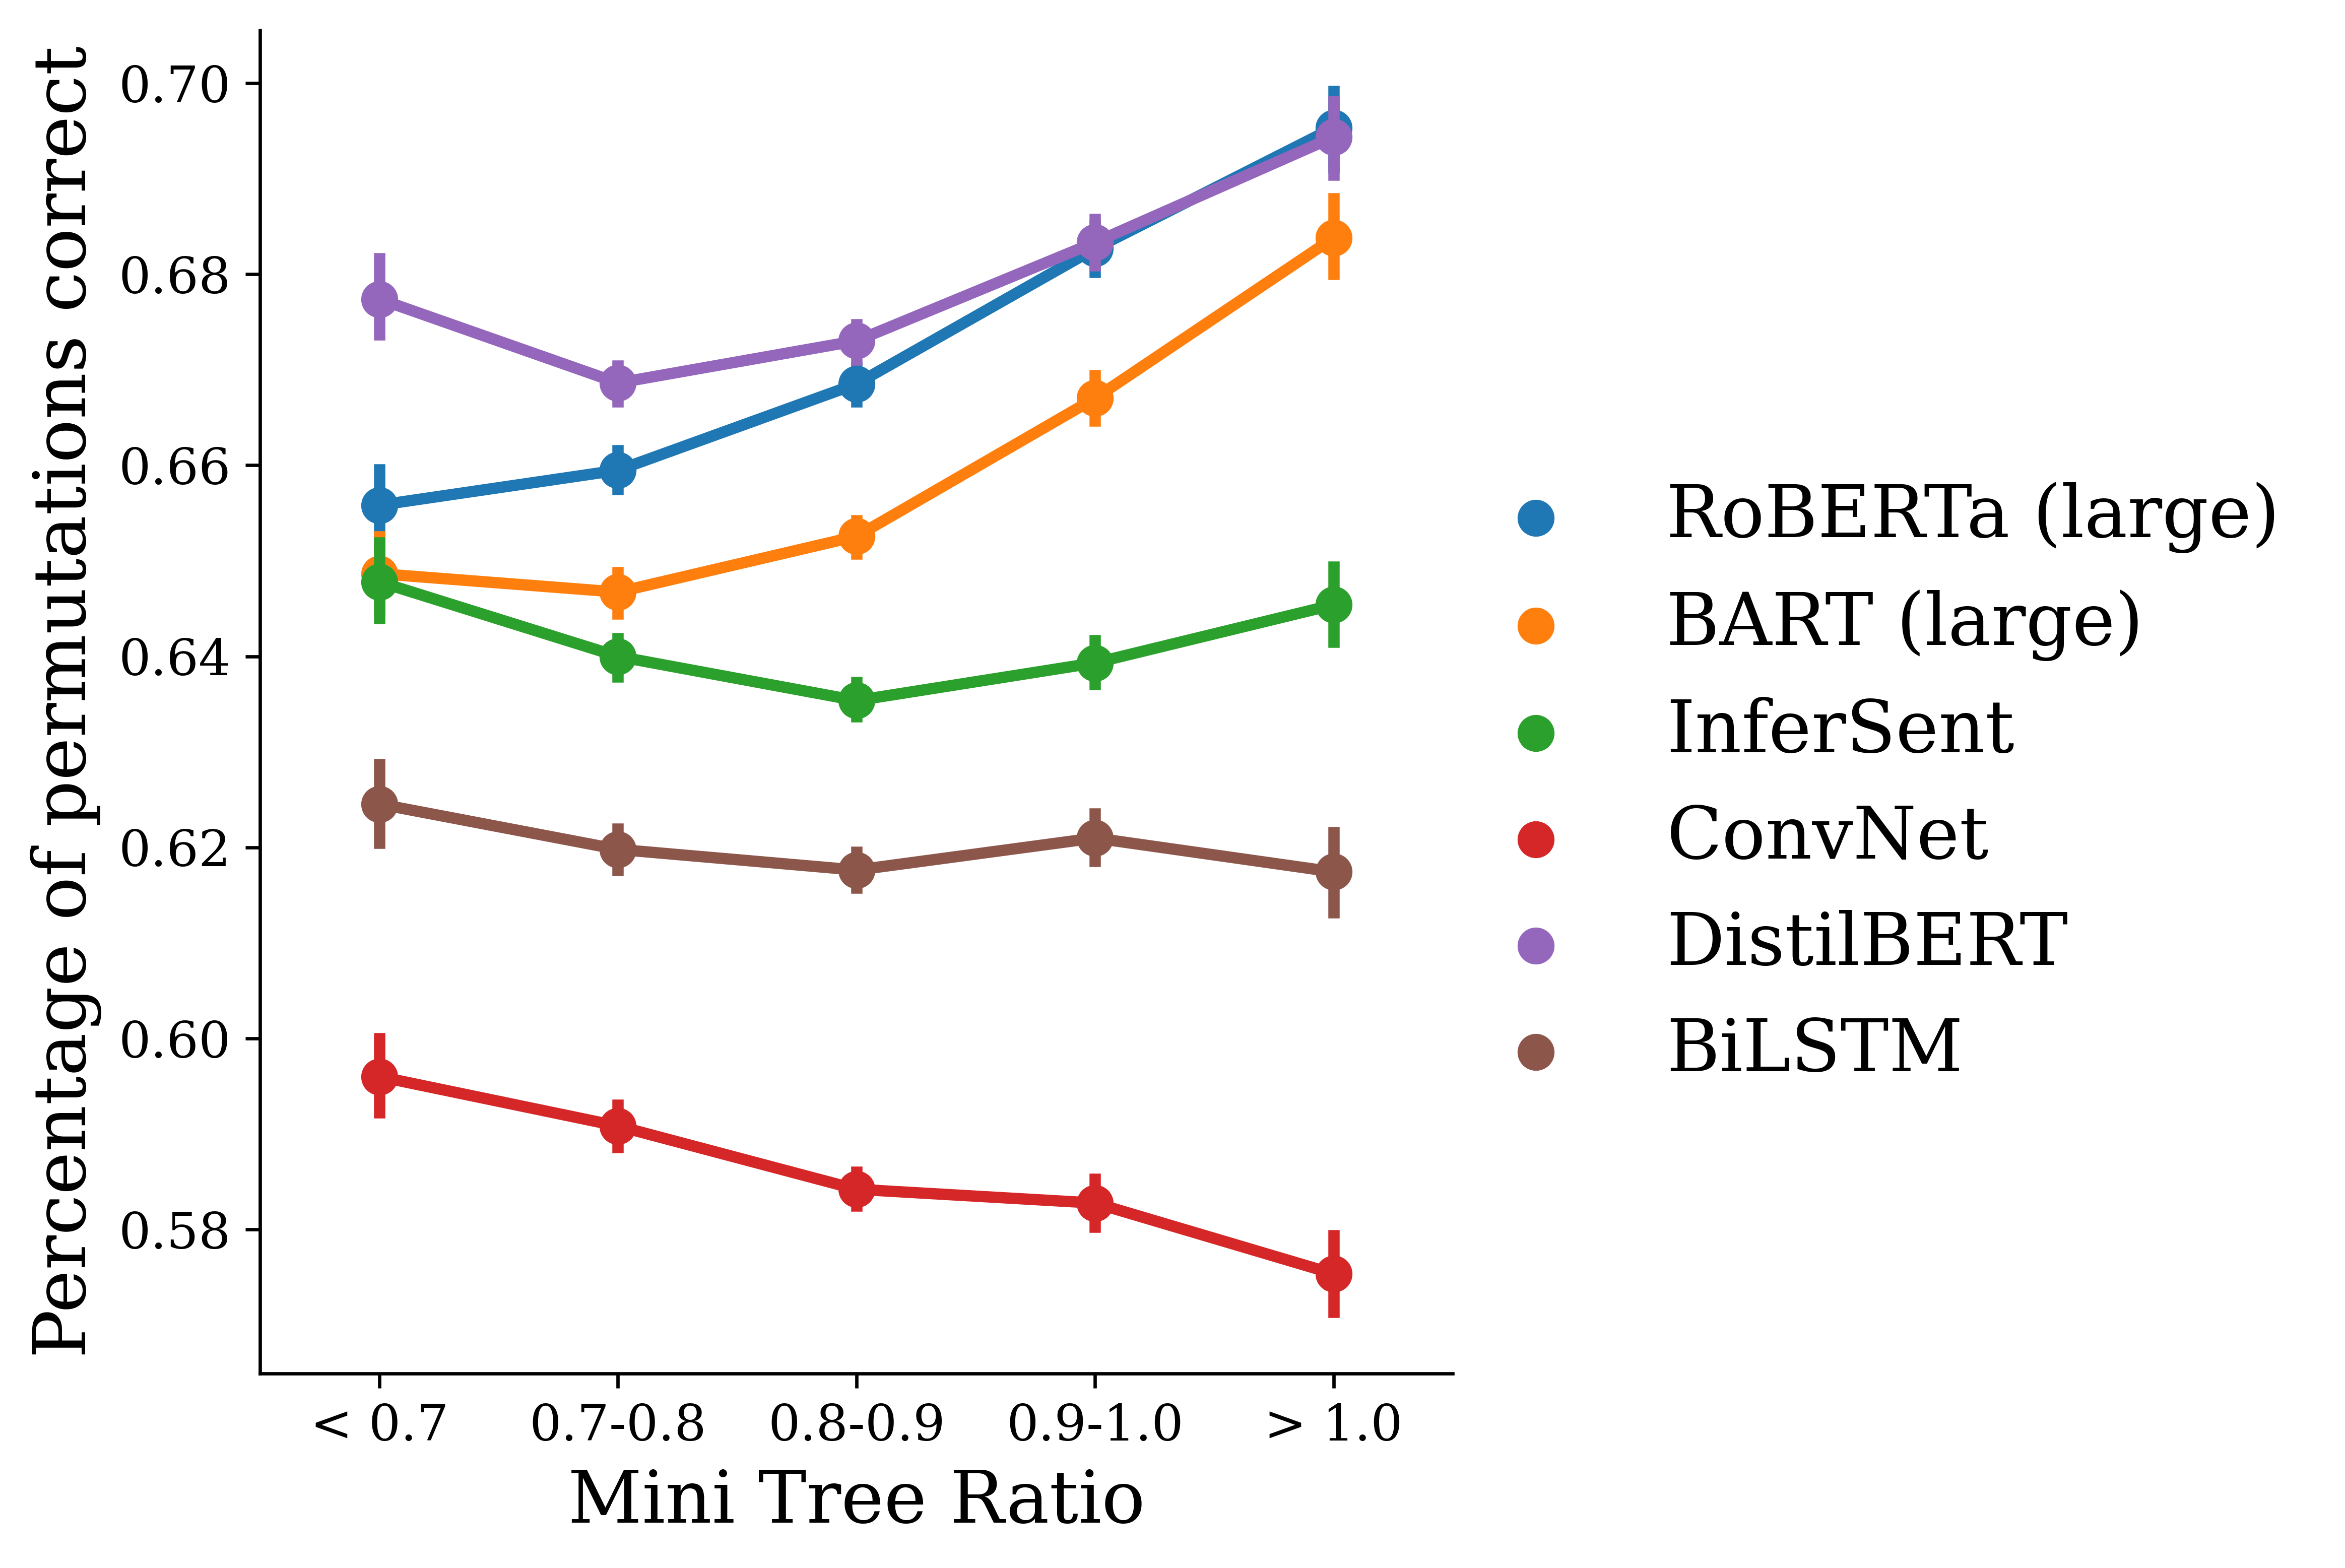
\includegraphics{figs/unli/min_tree_4.png}}
    \caption{POS Tag Mini Tree overlap score and  percentage of permutations which the models assigned the gold-label.}
    \label{fig:min_tree_4}
\end{figure}

We investigate the relationship with percentage of permuted sentences accepted with $\beta^k_{\{\hat{S}_i\}} / \beta^k_{\{S_i\}}$ in \autoref{fig:min_tree_4}. We observe that the POS Tag Minitree hypothesis holds for Transformer-based models, RoBERTa, BART and DistilBERT, where the percentage of accepted pairs increase as the sentences have higher overlap with the un-permuted sentence in terms of POS signature. For non-Transformer models such as InferSent, ConvNet, and BiLSTM models, the POS signature ratio to percentage of correct permutation remains the same or decreases, suggesting that the reasoning process employed by these models does not preserve local abstract syntax structure (i.e., POS neighbor relations).

%KS: Ideas: should we show POS tag correlation with original un-permuted sentences as well?

\subsection{Human Evaluation}
\label{sec:unli_human_eval}

%Since our models often accept permuted sentences, we ask how humans perform unnatural language inference on permuted sentences.
We expect humans to struggle with UNLI, given our intuitions and the sentence superiority findings (but see \citealt{mollica-2020-composition}). To test this, we presented two experts in NLI (one a linguist) with permuted sentence pairs to label.\footnote{Concurrent work by \cite{gupta-etal-2021-bert} found that untrained crowdworkers accept NLI examples that have been subjected to different kinds of perturbations at roughly most frequent class levels---i.e., only 35\% of the time.} Concretely, we draw equal number of examples from MNLI Matched dev set (100 examples where RoBERTa predicts the gold label, $D^c$ and 100 examples where it fails to do so, $D^f$), and then permute these examples using $\mathcal{F}$. The experts were given no additional information (recall that it is common knowledge that NLI is a roughly balanced 3-way classification task). Unbeknownst to the experts, all permuted sentences in the sample were actually accepted by the RoBERTa (large) model (trained on MNLI dataset). We observe that the experts performed much worse than RoBERTa (\autoref{tab:human_eval}), although their accuracy was a bit higher than random. We also find that for both experts, accuracy on permutations from $D^c$ was higher than on $D^f$, which verifies findings that showed high word overlap can give hints about the ground truth label \citep{dasgupta-etal-2018-evaluating, poliak-etal-2018-hypothesis, gururangan-etal-2018-annotation, naik-etal-2019-exploring}.

% Please add the following required packages to your document preamble:
% \usepackage{booktabs}
% \usepackage{graphicx}
\begin{table}[t]
\centering
\resizebox{0.7\linewidth}{!}{%
\begin{tabular}{@{}lllll@{}}
\toprule
Evaluator & Accuracy & Macro F1 & Acc on $D^{c}$ & Acc on $D^{f}$ \\ \midrule
X & 0.581 $\tiny\pm 0.068$ & 0.454 & 0.649 $\tiny\pm 0.102$ & 0.515 $\tiny\pm 0.089$ \\
Y &  0.378 $\tiny\pm 0.064$ & 0.378 & 0.411 $\tiny\pm 0.098$ & 0.349 $\tiny\pm 0.087$ \\ %\midrule
%crowd^{*} & & 0.35 & \\
\bottomrule
\end{tabular}%
}
\caption{Human (expert) evaluation on 200 permuted examples from the MNLI matched development set. Half of the permuted pairs contained shorter sentences and the other, longer ones. %Experts were provided only the permuted sentences (not the original example or the label) and were disallowed from consulting with one another. 
All permuted examples were assigned the gold label by RoBERTa-Large. %crowd$^*$ was crowdworker accuracy measured by \newcite{gupta-etal-2021-bert} on the GLUE Benchmark. 
}
\label{tab:human_eval}
\end{table}


\subsection{Training by Maximizing Entropy}
\label{sec:unli_training}
% training done on roberta.large.

We propose an initial attempt to mitigate the effect of correct prediction on permuted examples. As we observe in \autoref{sec:unli_results_conf}, model entropy on permuted examples is significantly lower than expected.
%This kind of phenomenon has been observed prior in Computer Vision \cite{gandhi2019mutual}, and suggests model struggle to to learn \textit{mutually exclusively}.
Neural networks tend to output higher confidence than random for even unknown inputs \cite{gandhi2019mutual}, which might be an underlying cause of the high \PermAcc.

% \begin{figure}
%     \centering
%     \resizebox{\linewidth}{!}{
%         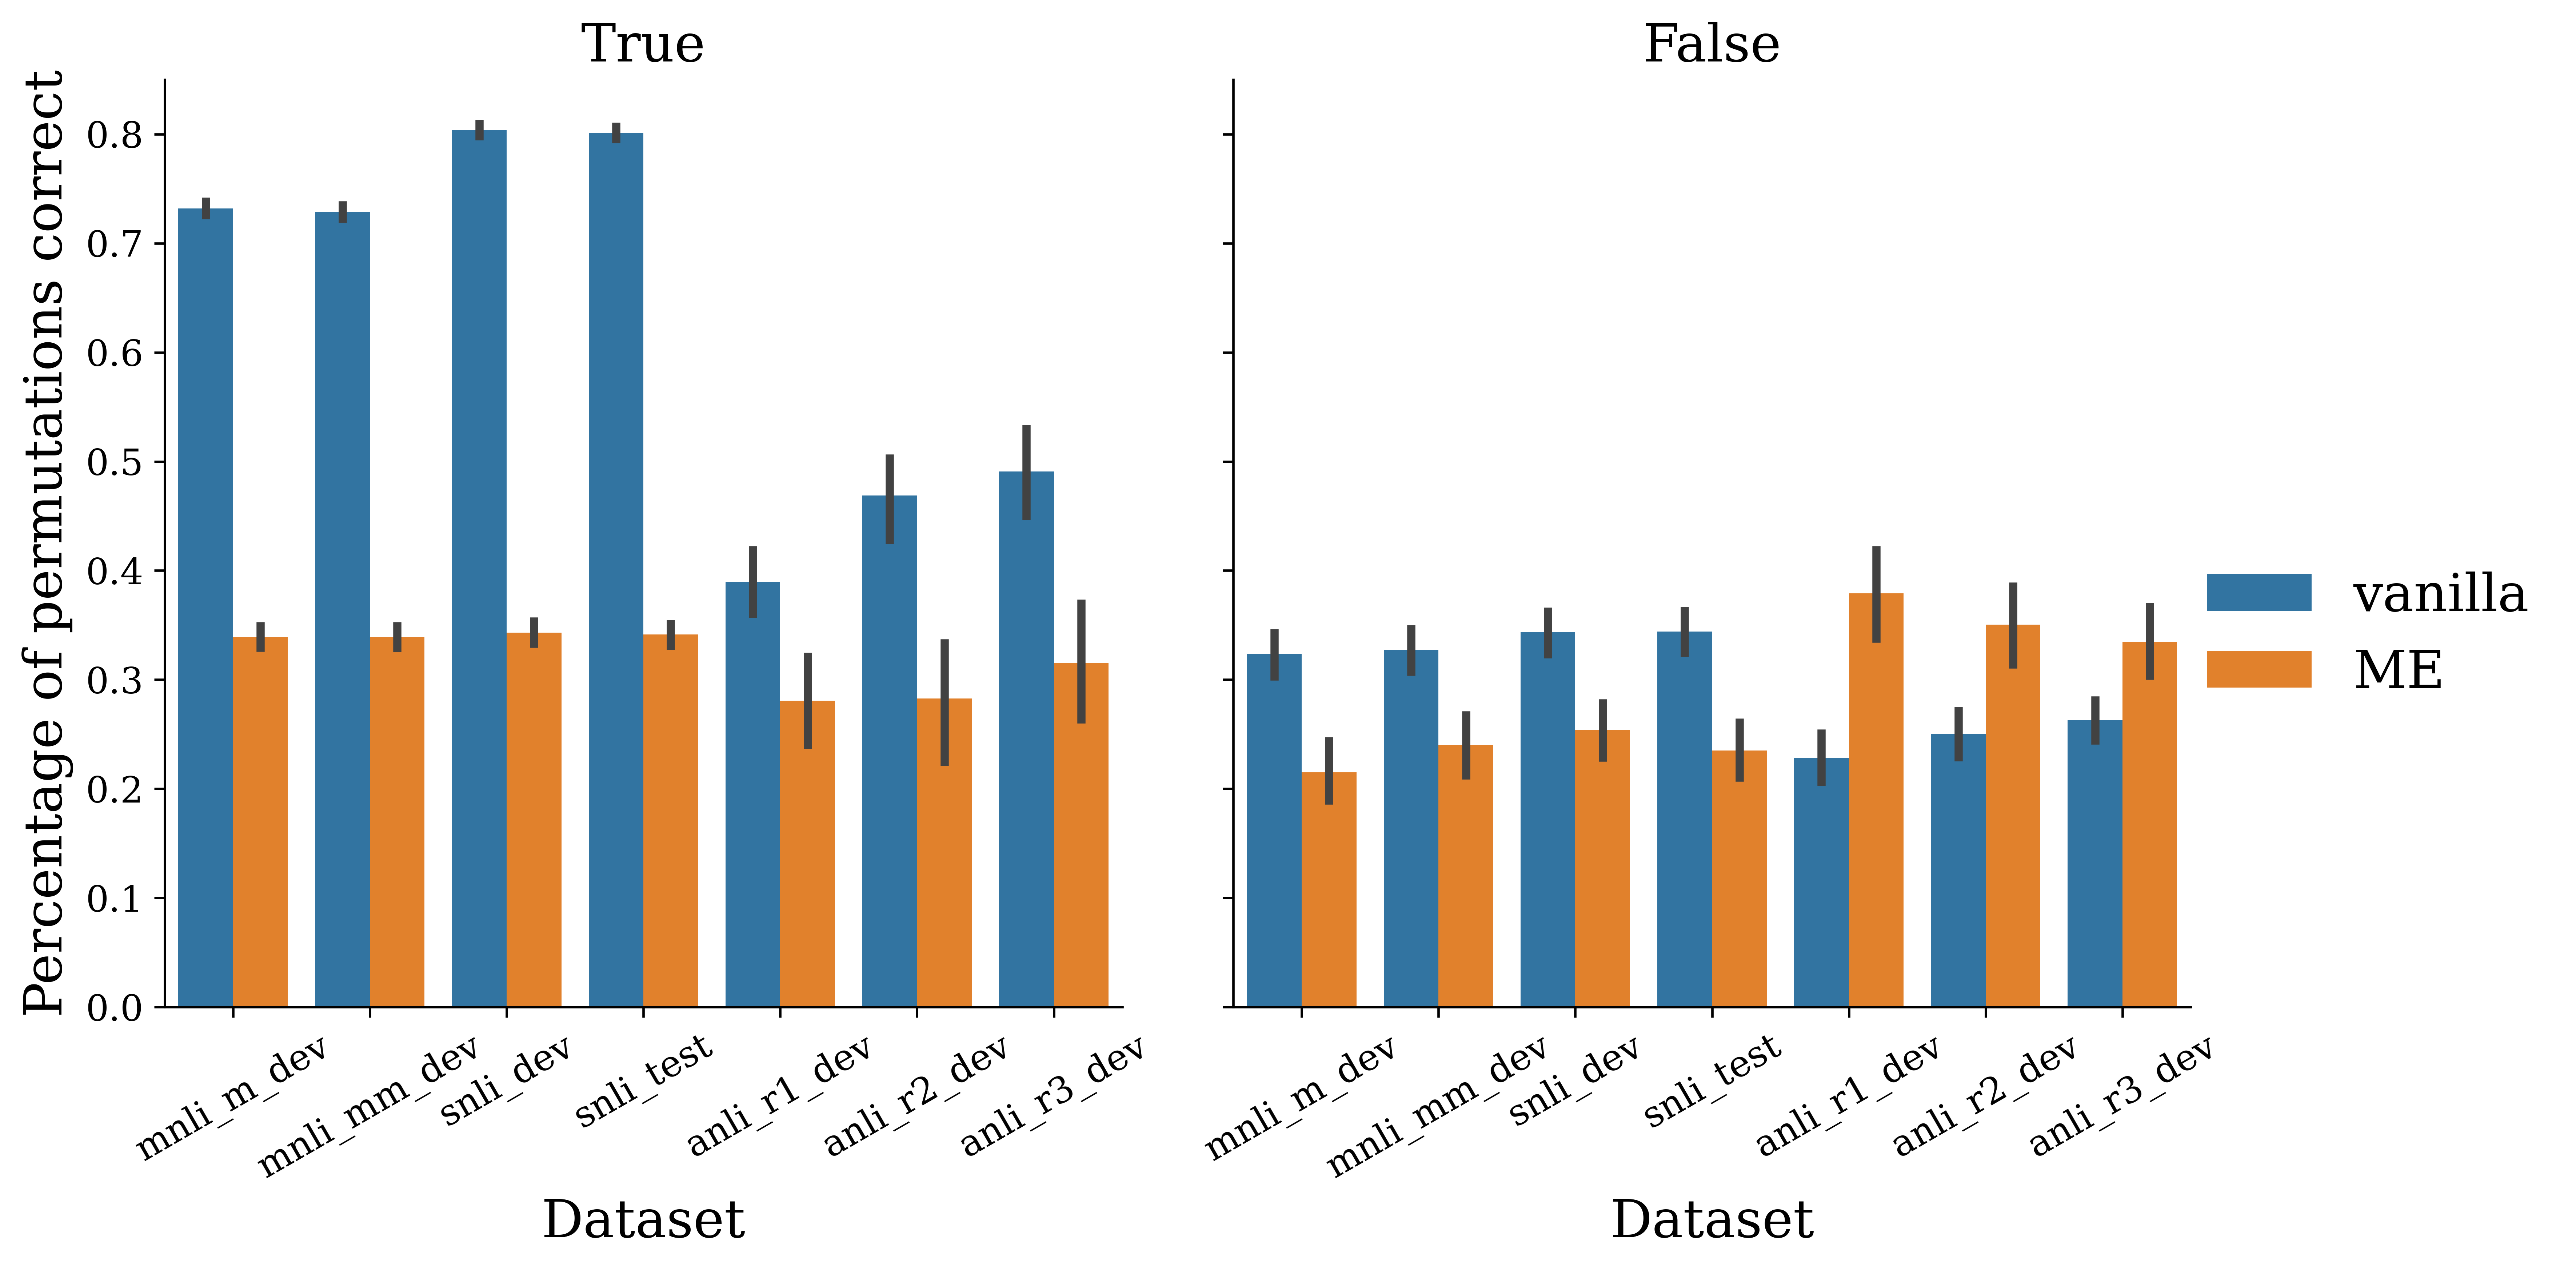
\includegraphics{images/me_train_roberta.png}}
%     \caption{Effect of maximizing entropy training on RoBERTa (large)}
%     \label{fig:max_ent_roberta}
% \end{figure.}

An ideal model would be ambivalent about randomized ungrammatical sentences. Thus, we train NLI models baking in the principle of mutual exclusivity \citep{gandhi2019mutual} by maximizing model entropy. Concretely, we fine-tune RoBERTa on MNLI while maximizing the entropy ($\bm{\mathcal{H}}$) on a subset of $n$ randomized examples ($(\hat{p}_i, \hat{r}_i$), for each example ($p,h$) in MNLI. We modify the loss function as follows:
% Prasanna
\begin{dmath}
    \mathcal{L}=\argminB_{\theta}\sum_{\left((p, h),y\right)}y\log(p(y|(p,h);\theta)) + \sum_{i=1}^n \bm{\mathcal{H}}\left(y|(\hat{p}_i,\hat{h}_i);\theta\right)
\end{dmath}
Using this maximum entropy method ($n=1$), we find that the model improves considerably with respect to its robustness to randomized sentences, all while taking no hit to accuracy (\autoref{table:ME_train_roberta}). We observe that no model reaches a $\Omega_{\text{max}}$ score close to 0, suggesting further room to explore other methods for decreasing models' \PermAcc. Similar approaches have also proven useful \citep{gupta-etal-2021-bert} for other tasks as well.

\begin{table}[t]
\centering
\resizebox{0.7\linewidth}{!}{%
\begin{tabular}{lrrrr}
\toprule
   Eval Dataset &   $\mathcal{A}$ (V) &  $\mathcal{A}$ (ME) &  $\Omega_{\text{max}}$ (V) &  $\Omega_{\text{max}}$ (ME) \\
\midrule
  MNLI\_m\_dev &  0.905 &     0.908 &    0.984 &        0.328 \\
 MNLI\_mm\_dev &  0.901 &     0.903 &    0.985 &        0.329 \\
   SNLI\_test &  0.882 &     0.888 &    0.983 &        0.329 \\
    SNLI\_dev &  0.879 &     0.887 &    0.984 &        0.333 \\
 ANLI\_r1\_dev &  0.456 &     0.470 &    0.890 &        0.333 \\
 ANLI\_r2\_dev &  0.271 &     0.258 &    0.880 &        0.333 \\
 ANLI\_r3\_dev &  0.268 &     0.243 &    0.892 &        0.334 \\
\bottomrule
\end{tabular}}
\caption{NLI Accuracy ($\mathcal{A}$) and \PermAcc\ metrics ($\Omega_{\text{max}}$) of RoBERTa when trained on MNLI dataset using vanilla (V) and Maximum Random Entropy (ME) method.}
  \label{table:ME_train_roberta}
\end{table}





\section{Related Work}
\label{sec:unli_related}

Researchers in NLP have realized the importance of syntactic structure in neural networks going back to \cite{tabor-1994-syntactic}. An early hand annotation effort on PASCAL RTE \citep{dagan-etal-2006} suggested that ``syntactic information alone was sufficient to make a judgment'' for roughly one third of examples %, whereas almost a half could be solved if annotators were additionally provided a thesaurus
\citep{vanderwende2005syntax}. %
Anecdotally, large generative language models like GPT-2 or -3 exhibit a seemingly humanlike ability to generate fluent and grammatical text \citep{goldberg2019assessing, wolf2019some}.
However, the jury is still out as to whether transformers genuinely acquire syntax.

\paragraph{Models appear to have acquired syntax.} When researchers have peeked inside Transformer LM's pretrained representations, familiar syntactic structure \citep{hewitt-manning-2019-structural,jawahar-etal-2019-bert, lin-etal-2019-open, warstadt-bowman-2020-can, wu-etal-2020-perturbed}, or a familiar order of linguistic operations \citep{jawahar-etal-2019-bert,  tenney-etal-2019-bert}, has appeared. There is also evidence, notably from agreement attraction phenomena \citep{linzen-etal-2016-assessing} that transformer-based models pretrained on LM do acquire some knowledge of natural language syntax \citep{gulordava-etal-2018-colorless, chrupala-alishahi-2019-correlating,  jawahar-etal-2019-bert, lin-etal-2019-open, manning-etal-2020-emergent,  hawkins-etal-2020-investigating, linzen-baroni-2021-syntactic}. Results from other phenomena \citep{warstadt-bowman-2020-can} such as NPI licensing  \citep{warstadt-etal-2019-investigating} lend additional support. The claim that LMs acquire some syntactic knowledge has been made not only for transformers, but also for convolutional neural nets \citep{bernardy-lappin-2017-using}, and RNNs \citep{gulordava-etal-2018-colorless, van-schijndel-linzen-2018-neural, wilcox-etal-2018-rnn, zhang-bowman-2018-language, prasad-etal-2019-using, ravfogel-etal-2019-studying}---although there are many caveats (e.g., \citealt{ravfogel-etal-2018-lstm, white-etal-2018-lexicosyntactic,  davis-van-schijndel-2020-recurrent, chaves-2020-dont, da-costa-chaves-2020-assessing, kodner-gupta-2020-overestimation}).

\paragraph{Models appear to struggle with syntax.} Several works have cast doubt on the extent to which NLI models in particular know syntax (although each work adopts a slightly different idea of what ``knowing syntax'' entails). For example, \cite{mccoy-etal-2019-right} argued that the knowledge acquired by models trained on NLI (for at least some popular datasets) is actually not as syntactically sophisticated as it might have initially seemed; some transformer models rely mainly on simpler, non-humanlike heuristics. In general, transformer LM performance has been found to be patchy and variable across linguistic phenomena \citep{dasgupta-etal-2018-evaluating, naik-etal-2018-stress, an-etal-2019-representation, ravichander-etal-2019-equate, jeretic-etal-2020-natural}. This is especially true for syntactic phenomena \citep{marvin-linzen-2018-targeted, hu-etal-2020-systematic, gauthier-etal-2020-syntaxgym, mccoy-etal-2020-berts, warstadt-etal-2020-blimp}, where transformers are, for some phenomena and settings, worse than RNNs \citep{van-schijndel-etal-2019-quantity}. From another angle, many have explored architectural approaches for increasing a network's sensitivity to syntactic structure \citep{chen-etal-2017-enhanced, Li-etal-2020-SANLI}. \cite{williams-etal-2018-latent} showed that learning jointly to perform NLI  and to parse resulted in parse trees that match no popular syntactic formalisms. Furthermore, models trained explicitly to differentiate acceptable sentences from unacceptable ones (i.e., one of the most common syntactic tests used by linguists) have, to date, come nowhere near human performance \citep{warstadt-etal-2019-neural}.

\paragraph{Insensitivity to Perturbation.} Most relatedly, several concurrent works \citep{pham-etal-2020-out, alleman2021syntactic, gupta-etal-2021-bert, sinha2021masked,parthasarathi2021sometimes} investigated the effect of word order permutations on transformer NNs.  \cite{pham-etal-2020-out} is very nearly a proper subset of our work except for investigating additional tasks (i.e. from the GLUE benchmark of \citealt{wang-etal-2018-glue}) and performing a by-layer-analysis. \cite{gupta-etal-2021-bert} also relies on the GLUE benchmark, but additionally investigates other types of ``destructive'' perturbations. Our contribution differs from these works %, although our tentative Maximum Entropy solution parallels a similar one in \newcite{}
in that we additionally include the following: we (i) outline theoretically-informed predictions for how models \emph{should be expected} to react to permuted input (we outline a few options), (ii) show that permuting can ``flip'' an incorrect prediction to a correct one, (iii) show that the problem isn't specific to Transformers, (iv) show that the problem persists on out of domain data, (v) offer a suite of flexible metrics, and (vi) analyze \emph{why} models might be accepting permutations (BLEU and POS-tag neighborhood analysis). Finally, we replicate our findings in another language.
% cite our two permutations papers & Yoon's student's in relation to our translation paper.
While our work (and \citeauthor{pham-etal-2020-out,gupta-etal-2021-bert}) only permutes data during fine-tuning and/or evaluation,
%raising the natural question: what is the result of permuting during training. \newcite{sinha2021masked} addresses this question.
recently \citeauthor{sinha2021masked} explored the sensitivity during pre-training, and found that models trained on n-gram permuted sentences perform remarkably close to regular MLM pre-training.
In the context of generation, \cite{parthasarathi2021sometimes} crafted linguistically relevant perturbations (on the basis of part-of-speech tagging and dependency parsing) to evaluate whether permutation hinders automatic machine translation models. Relatedly, but not for translation, \cite{alleman2021syntactic} investigated a smaller inventory of perturbations with emphasis on phrasal boundaries and the effects of n-gram perturbations on different layers in the network. % AW: Koustuv, please check this

% TODO: gururangan citation is double, check and remove

\paragraph{NLI Models are very sensitive to words.} NLI models often over-attend to particular words to predict the correct answer \citep{gururangan-etal-2018-annotation, clark-etal-2019-bert}. \cite{wallace-etal-2019-universal} show that some short sequences of non-human-readable text can fool many NLU models, including NLI models trained on SNLI, into predicting a specific label. In fact, \cite{ettinger-2020-whatbertisnot} observed that for one of three test sets, BERT loses some accuracy in word-perturbed sentences, but that there exists a subset of examples for which BERT’s accuracy remains intact.
%This led \citeauthor{ettinger-2020-whatbertisnot} to speculate that ``some of BERT's success on these items may be attributable to simpler lexical or n-gram information''. Thus, it is reasonable to wonder how well NLI models will perform on permuted sentences where the model is able to view the same collection of words.
If performance isn't affected (or if permutation helps, as we find it does in some cases), it suggests that these state-of-the-art models actually perform somewhat similarly to bag-of-words models \cite{blei-etal-2003-latent, mikolov2013efficient}.

% Todo: cite dasgupta et al
% Todo: cite goodwin et al



\section{Discussion}
\label{sec:unli_discussion}

In this chapter, we observe that state-of-the-art models do not rely on sentence structure the way we think they should: NLI models (Transformer-based models, RNNs, and ConvNets) are largely insensitive to permutations of word order that corrupt the original syntax. This raises questions about the extent to which such systems understand ``syntax'', and highlights the unnatural language understanding processes they employ. To summarize, our primary observations from this chapter are:

\begin{itemize}
  \item \textbf{\acrshort{nlu} models can still perform the task even if the word orders are scrambled} We observed overwhelming evidence in \autoref{sec:unli_results_accept} that state-of-the-art \acrshort{nlu} models tend to perform the task comparably even on word order scrambled text, which has no inherent semantic meaning.

  \item \textbf{Certain permutations allow \acrshort{nlu} models to flip classification labels, leading to better task scores.} We find that certain permutations of the order of words in a given input sentence pair can trigger the model to change the classification labels from the baseline, leading to large performance gains in the scores of the NLI task. For instance, in the examples which the models find difficult to predict, a permutation of the word order can elicit the model to assign the gold label.

  \item \textbf{\acrshort{nlu} models display rudimentary understanding of syntax, as evident by the preservation of abstract parts-of-speech neighborhood information.} We do find that models seem to have learned some syntactic information as is evidenced by a correlation between preservation of abstract POS neighborhood information and rate of acceptance by models, but these results do not discount the high rates of \PermAcc, and require further verification.

\end{itemize}


%While we have shown that classification labels can be flipped based solely on a sentence reordering, on interesting future direction to explore might be to additionally consider dropping tokens. Such an approach has been taken in the realm of interpretability to determine the impact of particular tokens on model decisions \citep{serrano-smith-2019-attention}. %% COMMENT OUT ABOVE FOR ARXIV SUBMIT.
% We also observe that reordering words can cause models to flip classification labels. % future work could additionally explore the relationship between permutation and deletion.
Given these findings, and coupled with the observation that humans cannot perform UNLI at all well, the high rate of permutation acceptance that we observe leads us to conclude that current models do not yet ``know syntax'' in the fully systematic and humanlike way we would like them to. This study leads us to further investigate the training dynamics employed by these large language models. In the next chapter, we will investigate the training data dependency of one such model family in detail, to shed more light on the sentence processing pipelines employed by these models.


% A few years ago, \cite{manning-etal-2015-computational} encouraged NLP to consider ``the details of human language, how it is learned, processed, and how it changes, rather than just chasing state-of-the-art numbers on a benchmark task.'' We expand upon this view, and suggest one particular future direction: we should train models not only to do well on clean test data, but also to not to overgeneralize to corrupted input. %perform natural language understanding in an humanlike way



\section{Follow-up findings in the community}
\label{sec:orgb976e8a}

\clearpage
\chapter{Probing syntax understanding through distributional hypothesis}
\label{sec:orgcdbaaa6}

Paper: \cite{sinha2021}

\section{Technical Background}
\label{sec:orgcfd03af}
\section{Dataset construction and pre-training}
\label{sec:orgc115e76}
\section{Experiments}
\label{sec:orgbbc65e2}
\subsection{Downstream reasoning tasks}
\label{sec:orge082779}

% \begin{figure}[htbp]
% \centering
% 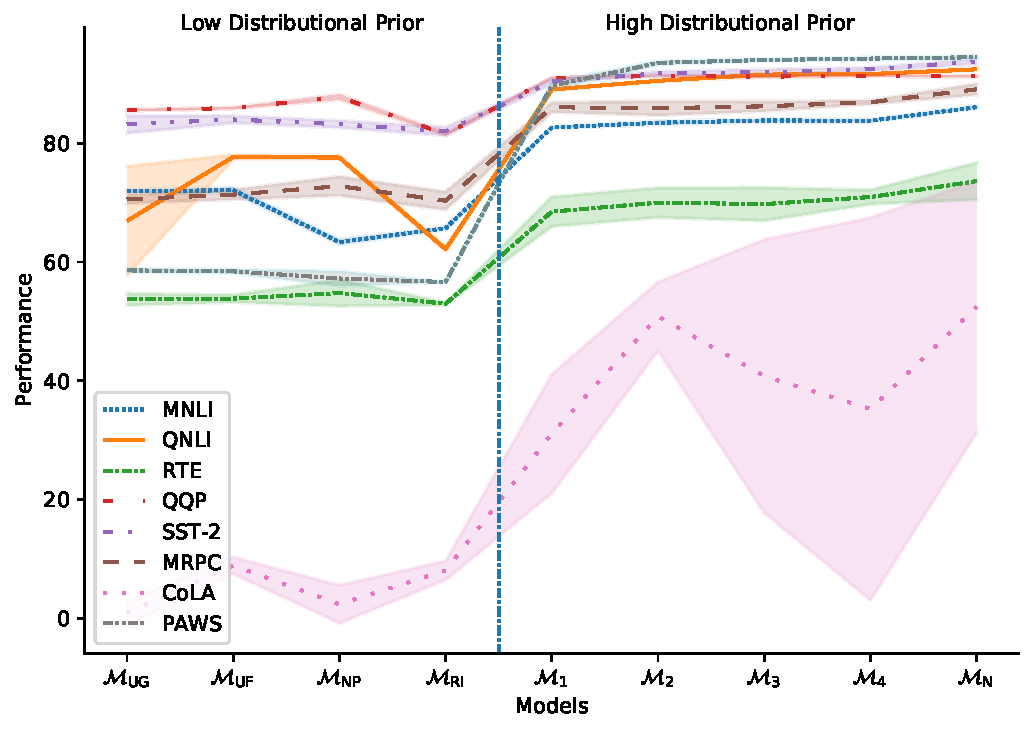
\includegraphics[width=.9\linewidth]{figs/unnat_pt/main_result_plot.pdf}
% \caption{Downstream results on scrambled pre-training.}
% \end{figure}

% \begin{figure}[htbp]
% \centering
% 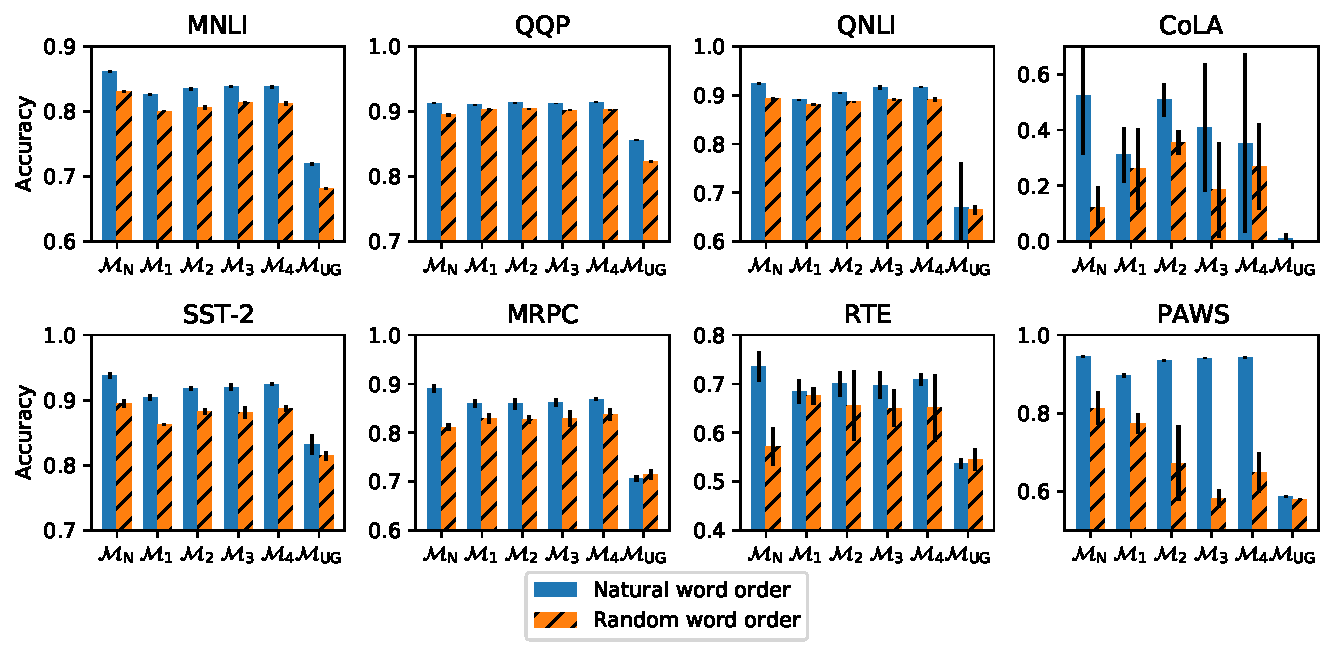
\includegraphics[width=.9\linewidth]{figs/unnat_pt/finetune_rand.pdf}
% \caption{GLUE and PAWS task dev set performance when finetuned on naturally and randomly ordered text, respectively, using pre-trained RoBERTa (base) models on different versions of BookWiki corpus.}
% \end{figure}

\subsection{Evaluating the effectiveness of probing syntax}
\label{sec:org56442b4}

% \begin{figure}[htbp]
% \centering
% 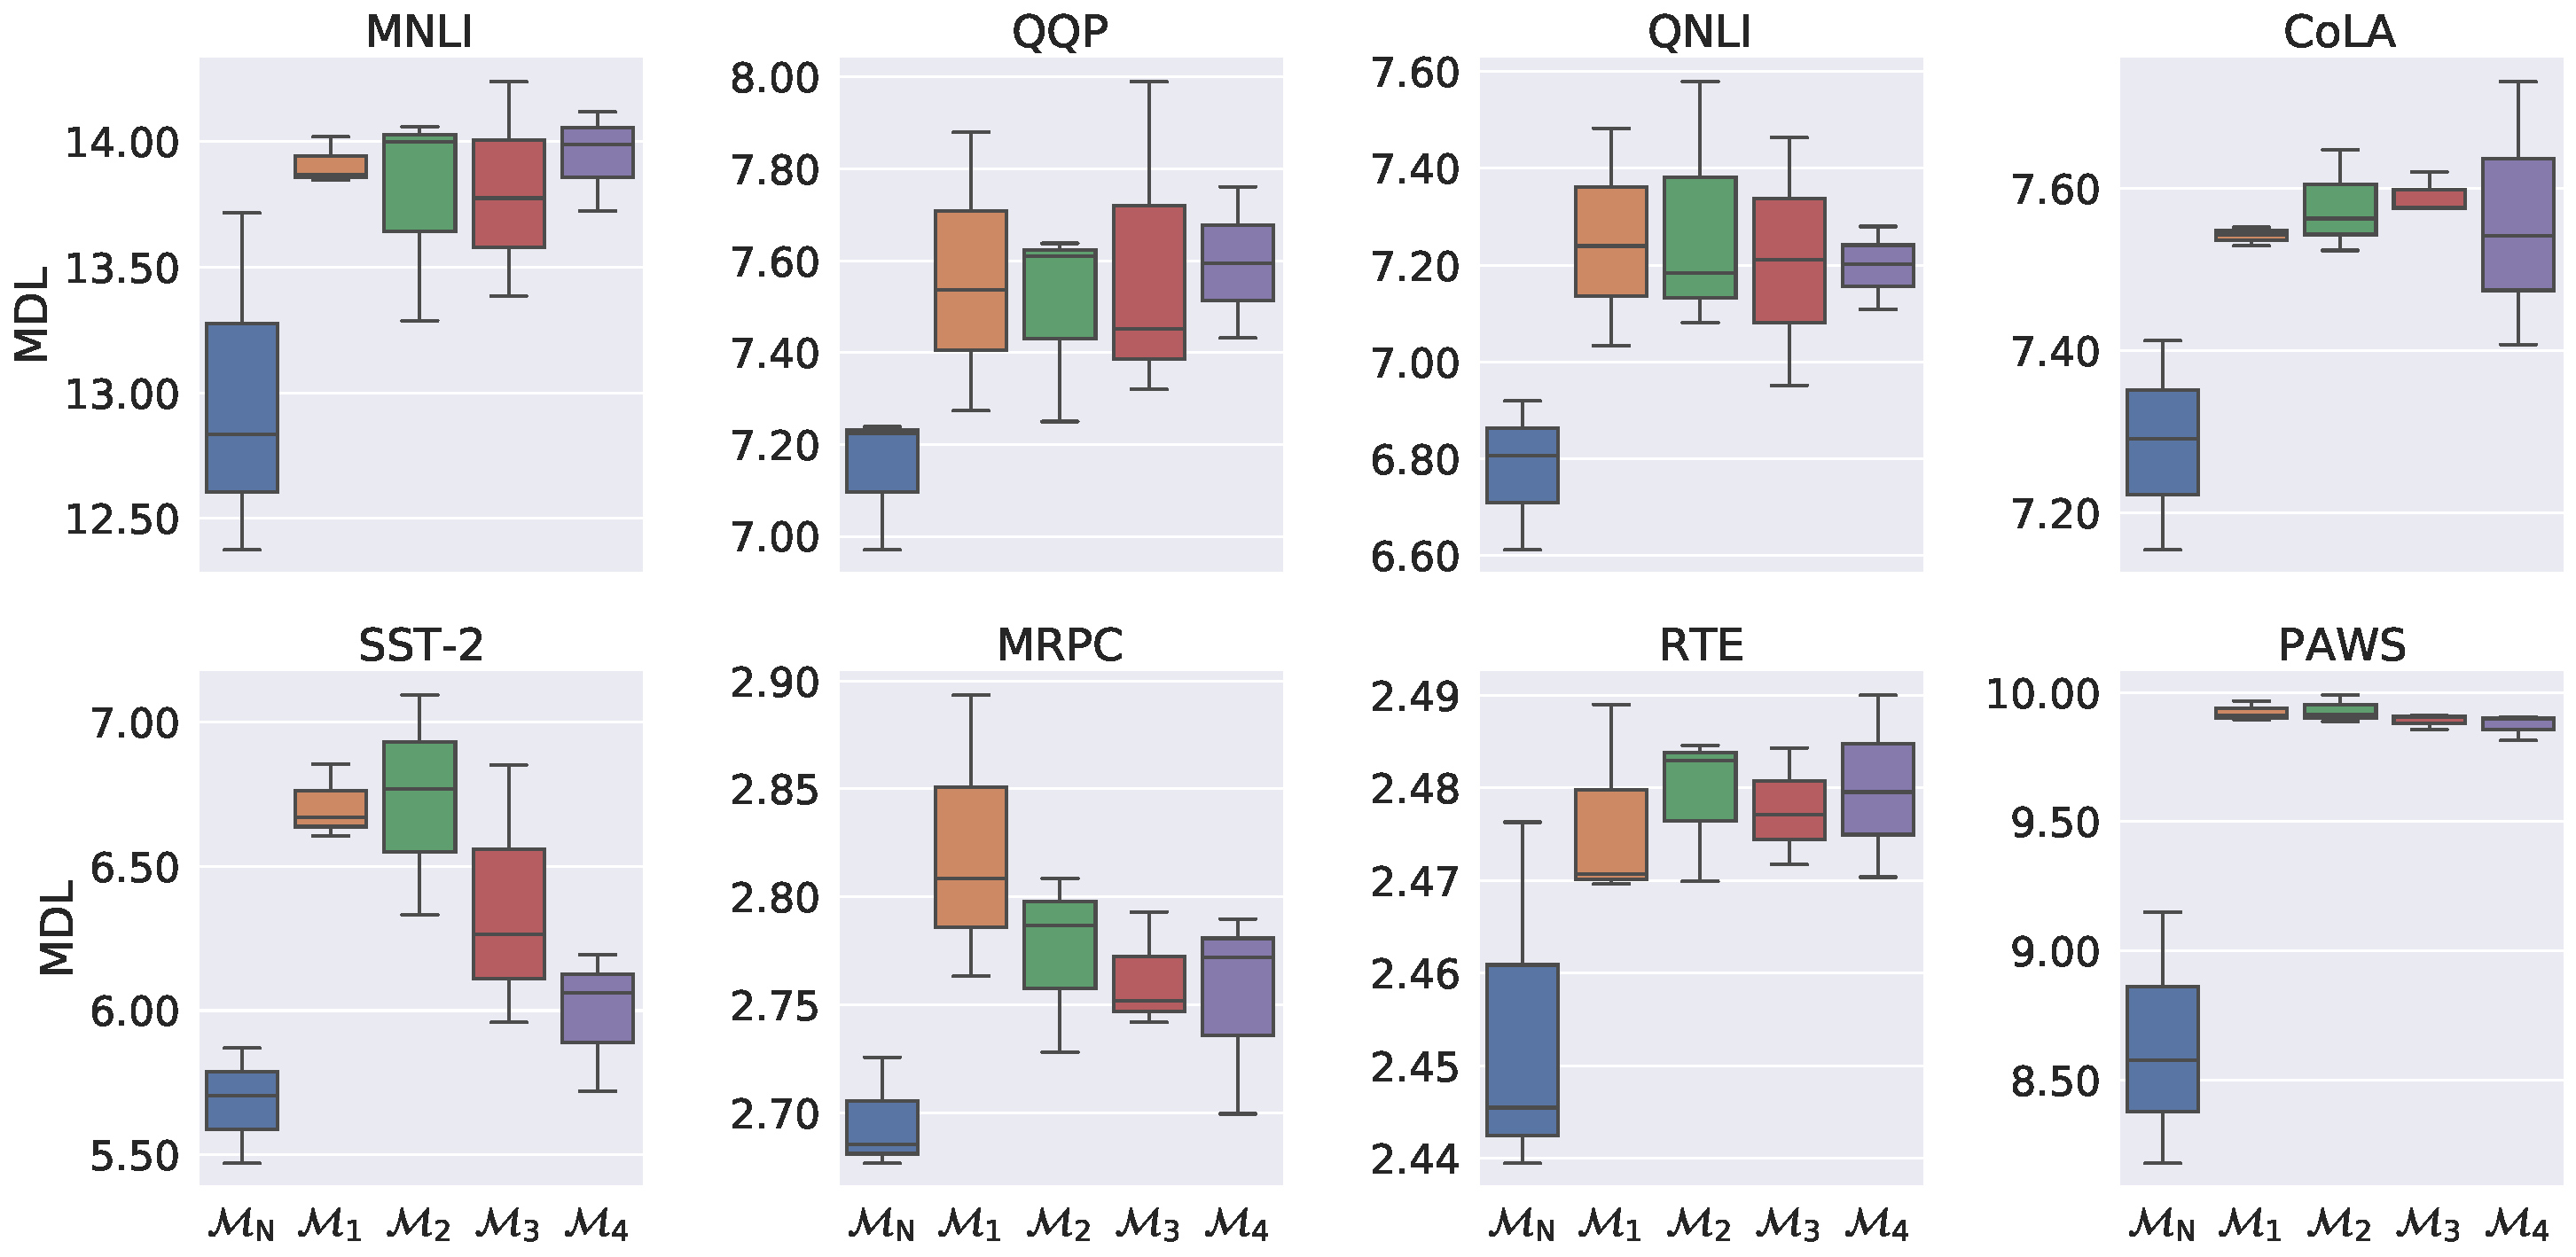
\includegraphics[width=.9\linewidth]{figs/unnat_pt/rda_mdl_ep_3.pdf}
% \caption{Risannen Data Analysis.}
% \end{figure}

\section{Related Work}
\label{sec:org0d2da32}
\section{Discussion}
\label{sec:org2941af9}
\section{Follow-up findings in the community}
\label{sec:orgde3bd47}
\clearpage
\chapter{Measuring systematic generalization by exploiting absolute positions}
\label{sec:orga46bf45}

\section{Technical Background}
\label{sec:orge8b9409}
\section{Systematic understanding of absolute position embeddings}
\label{sec:orgf8ea1d9}
\section{Related Work}
\label{sec:org05c8af6}
\section{Experiments}
\label{sec:orgc6f5de8}

% \begin{figure}[htbp]
% \centering
% 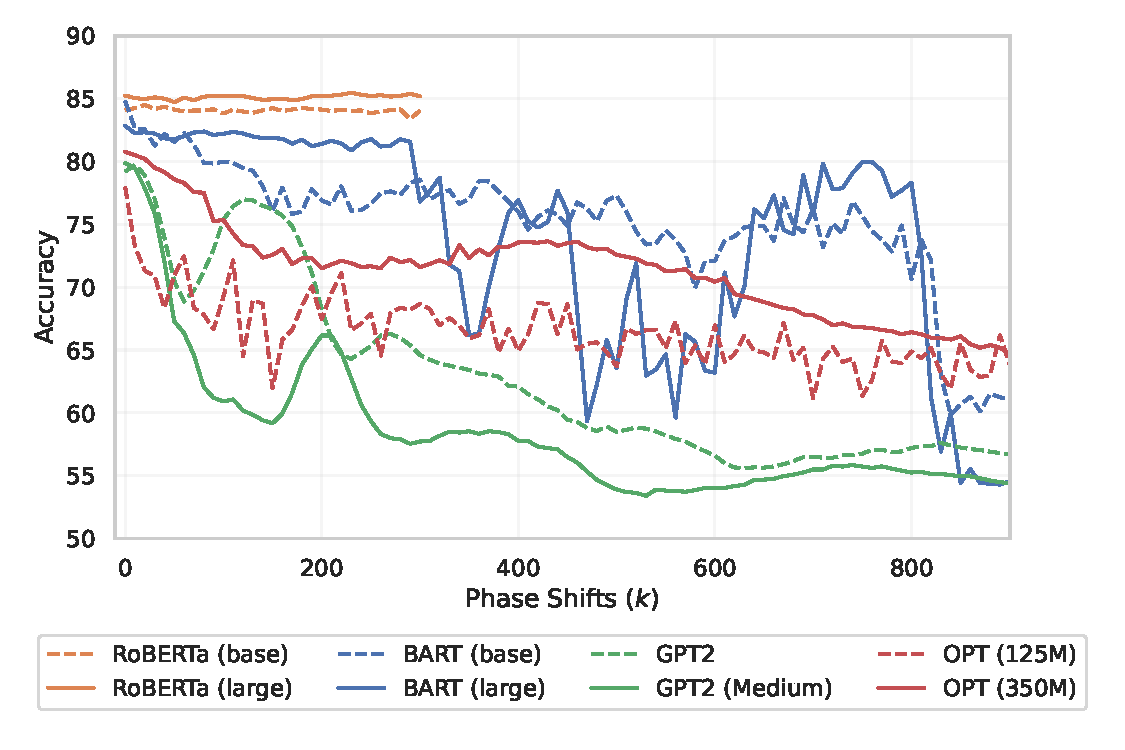
\includegraphics[width=.9\linewidth]{figs/pos_enc/acceptability_scores.pdf}
% \caption{Grammatical acceptability scores on BLiMP dataset.}
% \end{figure}

\section{Discussion}
\label{sec:orgbc43cdd}
\clearpage
\chapter{Conclusion}
\label{sec:org8fd280e}
\section{Summary}
\label{sec:org94aab9a}
\section{Limitations}
\label{sec:org217d56a}
\section{Future Work}
\label{sec:org9de237c}

\clearpage

\bibliographystyle{plainnat}
\bibliography{bibfiles/unli,bibfiles/clutrr,bibfiles/pos_enc,bibfiles/unnat_pt,bibfiles/anthology}


\printglossaries

\chapter{Appendix}
\label{sec:orgd5099eb}
\section{Org mode auto save}
\label{sec:orgde5798f}
Run the following snippet to auto save and compile in org mode.

\begin{verbatim}
(defun kdm/org-save-and-export ()
(interactive)
(if (and (eq major-mode 'org-mode)
    (ido-local-file-exists-p (concat (file-name-sans-extension (buffer-name)) ".tex")))
  (org-latex-export-to-latex)))

(add-hook 'after-save-hook 'kdm/org-save-and-export)
\end{verbatim}

\section{Remove ``parts'' from report}
\label{sec:orgacef247}

\begin{verbatim}
(add-to-list 'org-latex-classes
             '("report-noparts"
               "\\documentclass[11pt]{report}"
               ("\\chapter{%s}" . "\\chapter*{%s}")
               ("\\section{%s}" . "\\section*{%s}")
               ("\\subsection{%s}" . "\\subsection*{%s}")
               ("\\subsubsection{%s}" . "\\subsubsection*{%s}")))
\end{verbatim}

\section{Add newpage before a heading}
\label{sec:org122b99a}

\begin{verbatim}
(defun org/get-headline-string-element  (headline backend info)
  (let ((prop-point (next-property-change 0 headline)))
    (if prop-point (plist-get (text-properties-at prop-point headline) :parent))))

(defun org/ensure-latex-clearpage (headline backend info)
  (when (org-export-derived-backend-p backend 'latex)
    (let ((elmnt (org/get-headline-string-element headline backend info)))
      (when (member "newpage" (org-element-property :tags elmnt))
        (concat "\\clearpage\n" headline)))))

(add-to-list 'org-export-filter-headline-functions
             'org/ensure-latex-clearpage)

\end{verbatim}

\section{Glossary and Acronym build using Latexmk}
\label{sec:org94133e2}

Add the following snippet in the file ``\textasciitilde{}/.latexmkrc'': (Source: \url{https://tex.stackexchange.com/a/44316})

\begin{verbatim}
add_cus_dep('glo', 'gls', 0, 'run_makeglossaries');
add_cus_dep('acn', 'acr', 0, 'run_makeglossaries');

sub run_makeglossaries {
    my ($base_name, $path) = fileparse( $_[0] ); #handle -outdir param by splitting path and file, ...
    pushd $path; # ... cd-ing into folder first, then running makeglossaries ...

    if ( $silent ) {
        system "makeglossaries -q '$base_name'"; #unix
        # system "makeglossaries", "-q", "$base_name"; #windows
    }
    else {
        system "makeglossaries '$base_name'"; #unix
        # system "makeglossaries", "$base_name"; #windows
    };

    popd; # ... and cd-ing back again
}

push @generated_exts, 'glo', 'gls', 'glg';
push @generated_exts, 'acn', 'acr', 'alg';
$clean_ext .= ' %R.ist %R.xdy';
\end{verbatim}
\section{Citation style buffer local}
\label{sec:org97a37f4}

\begin{verbatim}
(set (make-local-variable 'bibtex-completion-format-citation-functions)
  '((org-mode      . my/bibtex-completion-format-citation-org-default-cite)))
\end{verbatim}
\section{Org latex compiler options}
\label{sec:orgc7e24c0}

\begin{verbatim}
(setq org-latex-pdf-process (list "latexmk -f -pdf -%latex -interaction=nonstopmode -output-directory=%o %f"))
\end{verbatim}

Original value

\begin{verbatim}
(setq org-latex-pdf-process (list "latexmk -f -pdf %f"))
\end{verbatim}

Let us try Fast compile \url{https://gist.github.com/yig/ba124dfbc8f63762f222}.

\begin{verbatim}
(setq org-latex-pdf-process (list "latexmk-fast %f"))
\end{verbatim}

\begin{itemize}
\item Doesn't seem to work from Emacs.
\item I need to change the save function to only export in tex. Then, have a separate process run latexmk.
\item Using the python package \texttt{when-changed} to watch the thesis.tex file for change.
\item Usage:
\end{itemize}

\begin{verbatim}
when-changed thesis.tex latexmk -f -pdf -interaction=nonstopmode -output-directory=%o thesis.tex
\end{verbatim}

\begin{itemize}
\item The pdf does not update. It seems to but not always? No it does. For some reason, compilation takes ages.
\item Works with \texttt{when-changed}!
\end{itemize}
\end{document}
